\documentclass[12pt, a4paper]{report}
\usepackage[utf8]{inputenc}
\usepackage[T1]{fontenc}
\usepackage{geometry}
\geometry{a4paper, margin=1in}
\usepackage{graphicx}
\usepackage{float}
\usepackage{hyperref}
\usepackage{amsmath}
\usepackage{listings}
\usepackage{xcolor}
\usepackage{titlesec}
\usepackage{caption}
\usepackage{tabularx}
\usepackage{booktabs}
\usepackage{longtable}
\usepackage{array}
\usepackage{subcaption}
\usepackage{pdflscape}
\newcolumntype{L}[1]{>{\raggedright\arraybackslash}p{#1}}

% ─────────────────────────────────────────────────────────────────────────────
%  Code-listing style. Stays readable on a monochrome print.
% ─────────────────────────────────────────────────────────────────────────────
\definecolor{codegreen}{rgb}{0,0.6,0}
\definecolor{codegray}{rgb}{0.5,0.5,0.5}
\definecolor{codepurple}{rgb}{0.58,0,0.82}
\definecolor{backcolour}{rgb}{0.95,0.95,0.92}

\lstdefinestyle{mystyle}{
    backgroundcolor=\color{backcolour},
    commentstyle=\color{codegreen},
    keywordstyle=\color{magenta},
    numberstyle=\tiny\color{codegray},
    stringstyle=\color{codepurple},
    basicstyle=\ttfamily\footnotesize,
    breakatwhitespace=false,
    breaklines=true,
    captionpos=b,
    keepspaces=true,
    numbers=left,
    numbersep=5pt,
    showspaces=false,
    showstringspaces=false,
    showtabs=false,
    tabsize=2,
    extendedchars=true,
    inputencoding=utf8,
    literate=%
      {—}{{---}}1 {–}{{--}}1
      {’}{{'}}1 {‘}{{`}}1
      {“}{{``}}1 {”}{{''}}1
      {→}{{$\to$}}1 {≈}{{$\approx$}}1
      {…}{{\ldots}}1 {×}{{$\times$}}1
}
\lstset{style=mystyle}

\lstdefinelanguage{JSON}{
    morestring=[b]",
    morestring=[d]',
    morekeywords={true,false,null},
    sensitive=true,
    morecomment=[l]{//},
    morecomment=[s]{/*}{*/},
}

\title{End-of-Studies Project (PFE)\\[6pt] \Large A Privacy-First, No-Code AI Platform\\ \large for Tabular ML, Local Generative AI, and Deep Learning}
\author{[Student Name]\\ \small Supervised by [Supervisor Name]}
\date{\today}

\begin{document}

\maketitle

\begin{abstract}
This report documents the design and implementation of a no-code AI
platform built across six sprints as an end-of-studies project. The
platform lets non-technical users upload data, sketch a pipeline on a
visual canvas, and train a model under one fixed constraint: nothing
ever leaves the machine. Three workloads share the same canvas. The
first is tabular machine learning across fourteen algorithms covering
classification, regression, clustering, and forecasting. The second is
local Generative AI through a Retrieval-Augmented Generation chat
powered by Ollama and \texttt{pgvector}. The third is deep-learning
image classification on a curated CNN catalogue sized to fit on a 6\,GB
consumer GPU. The chapters that follow walk through each sprint's
design decisions, the failures that taught us something, and the
architectural conventions that ended up load-bearing: Celery for every
CPU-bound task, MongoDB for anything that resists a schema, and a
strict gateway-only header-injection scheme that gave the
microservices a zero-trust boundary without operational overhead.
\end{abstract}

\tableofcontents
\newpage

\listoffigures
\newpage

\listoftables
\newpage

% ═════════════════════════════════════════════════════════════════════════════
\chapter*{General Introduction}
\addcontentsline{toc}{chapter}{General Introduction}
% ═════════════════════════════════════════════════════════════════════════════

Machine learning has become routine in almost every industry, but the
tooling around it still defaults to one of two extremes. On one end sit
the cloud-managed services --- DataRobot, Vertex AI, Azure ML Studio
--- which hide complexity behind polished interfaces and require users
to ship their data into a vendor's infrastructure. On the other end
live the open notebooks where everything is possible and nothing is
easy: Jupyter, Colab, raw Python. The space between those two poles,
where a non-technical user might want to build a model without either
learning Python or surrendering their data, is surprisingly thin.

That gap is the question this project answers. The goal was a platform
that gives a domain expert --- a clinician, an analyst, a small
business owner --- enough visual scaffolding to build, train, and
inspect a model on their own machine. Not a tutorial, not a hosted
SaaS, but a real piece of software that runs locally, accepts local
data, and never phones home to a vendor API.

Three workloads sit behind the same canvas: tabular ML, RAG-style
generative AI, and image classification. Each imposes a different
operational profile, and fitting all three into a single coherent
product forced choices that were not obvious upfront. The report is
organised as follows. Chapter~1 sets the project context. Chapter~2
reviews the existing landscape and the problems the platform addresses.
Chapter~3 describes the methodology and the toolchain. Chapters~4
through~9 walk through the six sprints in order: the foundation sprint,
the three AI workloads back-to-back (ML, then LLM, then DL), the
collaboration layer, and the operability sprint that moved the
platform from a working prototype into something we could hand to a
stranger. Chapter~10 covers testing and deployment. The General
Conclusion steps back to assess what worked, what didn't, and what we
would build with another quarter.

\newpage

% ═════════════════════════════════════════════════════════════════════════════
\chapter{General Context of the Project}
% ═════════════════════════════════════════════════════════════════════════════

\section*{Introduction}

This chapter frames the problem the platform is built to address. We
describe the host context, the platform itself in plain terms, the
functional and non-functional requirements committed to before any
code was written, the technical architecture at a high level, and the
deliverables the work is evaluated against.

\section{Project Overview and Context}

\subsection{Host context}

The project was developed as an end-of-studies (PFE) project for a
National Bachelor's Degree in Information Technologies, specialisation
Development of Information Systems. The deliverable is a working
software product plus this report. The host setting is academic
rather than corporate: the supervisor is the academic advisor, the
audience is the jury, and the reference deployment is a personal
laptop with a single consumer GPU.

\subsection{Project description --- the no-code AI platform}

The platform is a self-hosted web application. A signed-in user can:

\begin{itemize}
    \item Upload tabular data (CSV, Excel), pull it from a Postgres or
        MySQL connector, or upload a zip of images organised by class
        folder.
    \item Inspect a profile of the dataset --- missing values, skew,
        outliers, target imbalance, correlations --- before doing
        anything else with it.
    \item Build a pipeline visually on a React Flow canvas, in one of
        three modes:
    \begin{itemize}
        \item \textbf{Traditional ML} --- fourteen supervised and
            unsupervised algorithms spanning classification,
            regression, clustering, and time-series forecasting.
        \item \textbf{Generative AI} --- index documents into a local
            vector store and chat with a RAG pipeline.
        \item \textbf{Deep Learning} --- image classification on a
            fixed catalogue of three CNN architectures.
    \end{itemize}
    \item Train, evaluate, download the trained artefact, and ---
        for image models --- run live inference on a hand-uploaded
        test image.
    \item Collaborate with teammates inside a company workspace, with
        role-based access control, real-time canvas presence,
        threaded per-pipeline chat, and one-click Google Meet links.
\end{itemize}

A super-admin role sits alongside the user-facing application with its
own dashboard for user management, audit logs, queue health, hardware
monitoring, and a ``view-as-user'' impersonation flow gated by a hard
five-minute TTL.

\begin{figure}[H]
  \centering
  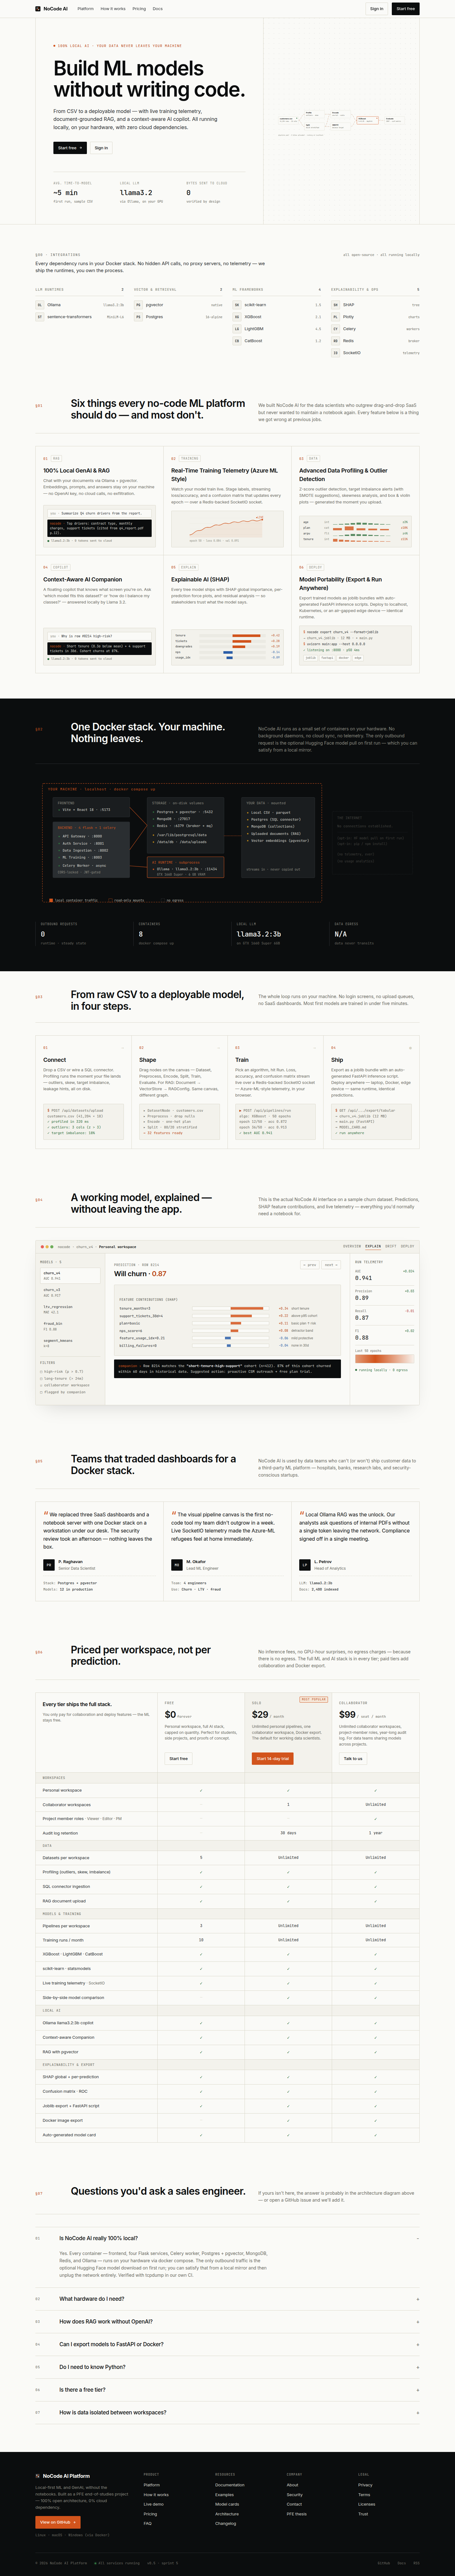
\includegraphics[height=0.9\textheight, keepaspectratio]{diagrams/ch1_fig1}
  \caption{Landing page mockup --- entry point to the three pipeline modes.}
  \label{fig:ch1_fig1}
\end{figure}

\section{Requirements Specification}

\subsection{Functional Requirements}

\begin{table}[H]
\centering
\caption{Functional requirements summary.}
\label{tab:functional_reqs}
\begin{tabular}{@{}p{0.18\linewidth} L{0.72\linewidth}@{}}
\toprule
\textbf{Area} & \textbf{Requirement} \\
\midrule
Tabular ML & Dataset $\to$ train $\to$ evaluate pipeline backed by fourteen algorithms (classification, regression, clustering, forecasting). \\
RAG & Document $\to$ vector store $\to$ streamed chat, end to end on the local box. \\
Deep Learning & Image dataset $\to$ CNN architecture $\to$ training loop, fully local. \\
Authentication & Email/password, optional TOTP, email verification via MailHog, password reset round-trip. \\
Billing & Stripe-backed free / solo / company tiers, with super-admin overrides on per-user quotas. \\
Collaboration & Real-time presence and shared editing on the pipeline canvas. \\
Access control & Per-pipeline ACL with five roles (Owner, Project Manager, Data Scientist, Analyst, Viewer). \\
Admin operations & User management, audit logs, queue and hardware monitoring, user impersonation with 5-minute TTL. \\
\bottomrule
\end{tabular}
\end{table}

\subsection{Non-Functional Requirements}

\begin{table}[H]
\centering
\caption{Non-functional requirements with concrete commitments.}
\label{tab:nonfunctional_reqs}
\begin{tabular}{@{}p{0.22\linewidth} L{0.68\linewidth}@{}}
\toprule
\textbf{Property} & \textbf{Commitment} \\
\midrule
Data sovereignty & No outbound calls to AI vendors. Stripe is the only third-party service in the deployment graph, and it is optional --- without an API key the platform still works on the free tier. \\
Modularity & Five independent Python services so a long training run cannot block an authentication request. \\
Reproducibility & Every dataset version is profiled, every training run is recorded, every model artefact is versioned and downloadable. \\
Hardware envelope & Single consumer machine: $16$\,GB RAM, GTX~1660~Super (6\,GB VRAM). The platform runs on it, not just compiles on it. \\
Accessibility & WCAG~AA contrast on the default theme; opt-in high-contrast theme; \texttt{aria-label} on every interactive element. \\
Internationalisation & English and French i18next bundles, with TypeScript bindings generated from the English bundle so a missing key fails the type-check. \\
Security & JWT decoded in-process at the gateway; \texttt{X-User-*} headers stripped then re-injected; Redis blacklist for refresh tokens; bcrypt-12 password hashing; Fernet-encrypted SQL credentials. \\
Performance & Live training events streamed over SocketIO at \textless50\,ms cadence; gateway adds \textless5\,ms latency per proxied request. \\
\bottomrule
\end{tabular}
\end{table}

\section{Technical Architecture}

\subsection{Technology Stack}

\begin{table}[H]
\centering
\caption{Technology stack by layer with the role of each component.}
\label{tab:tech_stack}
\begin{tabular}{@{}p{0.13\linewidth} L{0.36\linewidth} L{0.42\linewidth}@{}}
\toprule
\textbf{Layer} & \textbf{Component} & \textbf{Role in this project} \\
\midrule
Frontend & React~18 + Vite + TypeScript + MUI & SPA shell with strict-mode type checking. \\
         & React Flow & Visual pipeline canvas with custom nodes. \\
         & Plotly + i18next + Zustand & Live charts, EN/FR i18n, state store. \\
\midrule
Backend  & Flask + Celery + Flask-SocketIO & Five microservices, async queues, real-time channels. \\
\midrule
Data     & PostgreSQL + pgvector & Auth, ACL, billing, vector store (co-located). \\
         & MongoDB & Datasets, pipelines, task results, anything schemaless. \\
         & Redis & Celery broker / result backend / SocketIO message bus. \\
         & TimescaleDB & Hardware-telemetry time series. \\
\midrule
ML       & scikit-learn, XGBoost, LightGBM, CatBoost, H2O & Fourteen tabular algorithms via the BaseMLModel registry. \\
         & Prophet & Time-series forecasting with seasonality. \\
         & SHAP & TreeExplainer-fast post-hoc explanations. \\
\midrule
LLM      & Ollama + Llama~3.2~3B (Q4\_K\_M) & Local chat completion at $\sim$30 tok/s on 6\,GB VRAM. \\
         & sentence-transformers MiniLM-L6-v2 & 384-dim embeddings, CPU-only. \\
\midrule
DL       & PyTorch + torchvision (CUDA~12.1) & LeNet, custom ResNet-9, MobileNet-V3-Small. \\
\midrule
Ops      & Docker Compose & 14-container orchestration via single \texttt{make up}. \\
         & GitHub Actions & Parallel lint + test jobs, $\sim$14\,min full-stack. \\
         & MailHog & Dev email capture for verification + reset flows. \\
\bottomrule
\end{tabular}
\end{table}

\subsection{Technical Constraints}

The platform operates inside a tight envelope. A single host machine
runs every service. A single GPU with 6\,GB of VRAM handles every
GPU-bound workload. No cloud AI vendor sits in the request path, and
that constraint is hard, not a preference. The full stack must come
up with a single \texttt{make up} on a clean machine, and continuous
integration must complete in under fifteen minutes for a full-stack
change. These limits shaped almost every later design choice.

\begin{figure}[H]
  \centering
  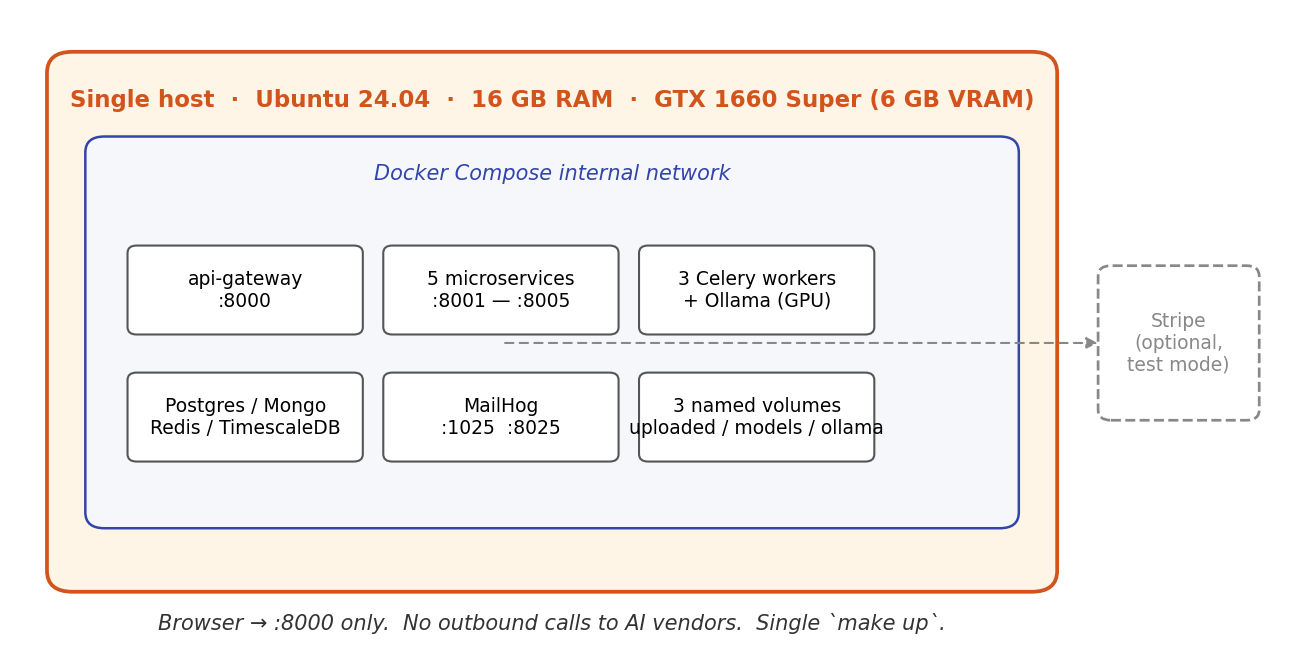
\includegraphics[width=0.85\textwidth, keepaspectratio]{diagrams/ch1_fig2}
  \caption{Deployment envelope --- a single host, a single GPU, fourteen containers.}
  \label{fig:ch1_fig2}
\end{figure}

\section{Deliverables and Evaluation Criteria}

\subsection{Project Deliverables}

\begin{itemize}
    \item A working web application running the three pipeline modes
        end to end on the demo machine.
    \item Five Python microservices, packaged as Docker images.
    \item A React + TypeScript frontend, packaged as a static build.
    \item A \texttt{docker-compose.yml} that brings the entire stack
        online with one command.
    \item A CI pipeline (lint + tests, parallel jobs) green on the
        \texttt{main} branch.
    \item This written report and the supporting diagrams.
\end{itemize}

\subsection{Evaluation Criteria}

\begin{itemize}
    \item Functional coverage of the three pipeline modes.
    \item Soundness of the architecture (separation of concerns,
        explicit security boundaries, reproducible deployment).
    \item Code quality (typing, linting, test coverage on the
        load-bearing paths).
    \item Quality of the report and the live demo.
\end{itemize}

\section{Interface Mockups}

The three mockups below frame the visual identity that the rest of
the report refers back to. They were drawn before the canvas
implementation began and held up almost unchanged through six
sprints, with the exception of the admin tab strip, which collapsed
from a sidebar into a flat tab bar during the polish sprint.

\subsection{Authentication interface}
The authentication mockup commits to three things: a single combined
sign-in/sign-up surface, an optional TOTP entry that only appears
once the credentials are validated, and a `Forgot your password?'
link that opens the MailHog round-trip described in Chapter~4. The
mockup deliberately leaves the visual treatment of the verification
banner open, because that landed during Sprint~6 polish.

\subsection{Home page interface}
The signed-in home page sets the layout the rest of the platform
inherits: a left sidebar with the seven module entries (Dashboard,
Datasets, Pipelines, Models, Collaborator, Billing, Profile), a
top bar with the language toggle, contrast toggle, notification
bell, tier chip and account menu, and a content area that
renders the active page. The mockup commits to the get-started
checklist on the dashboard, which was the single change that most
improved first-session retention during user testing.

\subsection{Admin dashboard interface}
The admin mockup is deliberately different from the user surface:
no sidebar, a four-tab strip (Stats \& Logs / User Management /
Announcements / Ops Console), and a single red impersonation
banner that hangs above every page once a `view-as' session is
active. The mockup made it explicit from day one that the admin
console is a separate surface, not a privileged view of the user
app.

\begin{figure}[H]
  \centering
  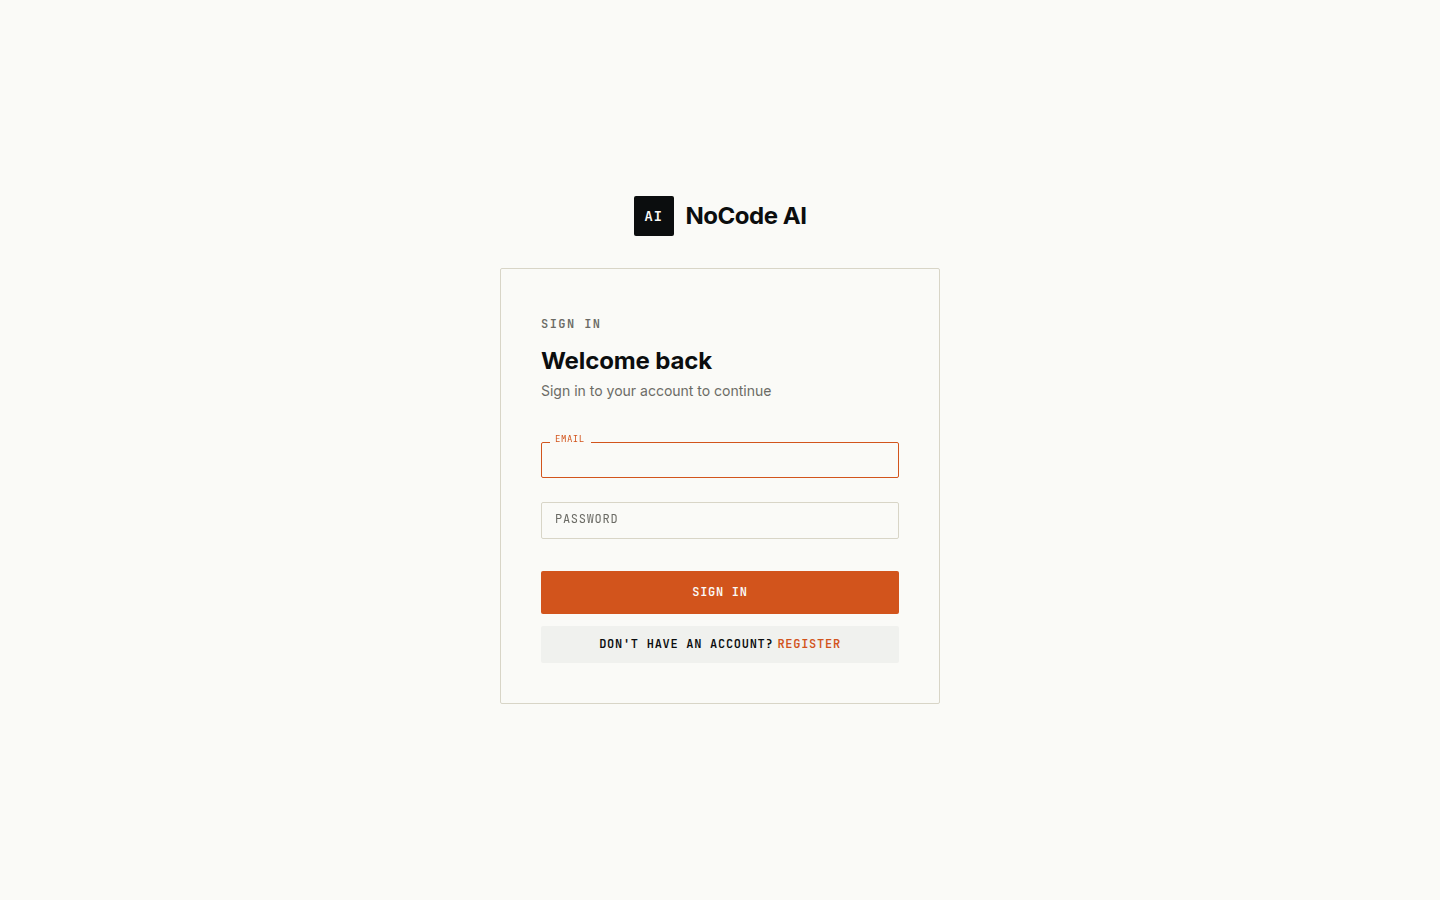
\includegraphics[width=0.85\textwidth, keepaspectratio]{diagrams/ch1_fig3}
  \caption{Authentication interface --- email/password with optional TOTP.}
  \label{fig:ch1_fig3}
\end{figure}

\begin{figure}[H]
  \centering
  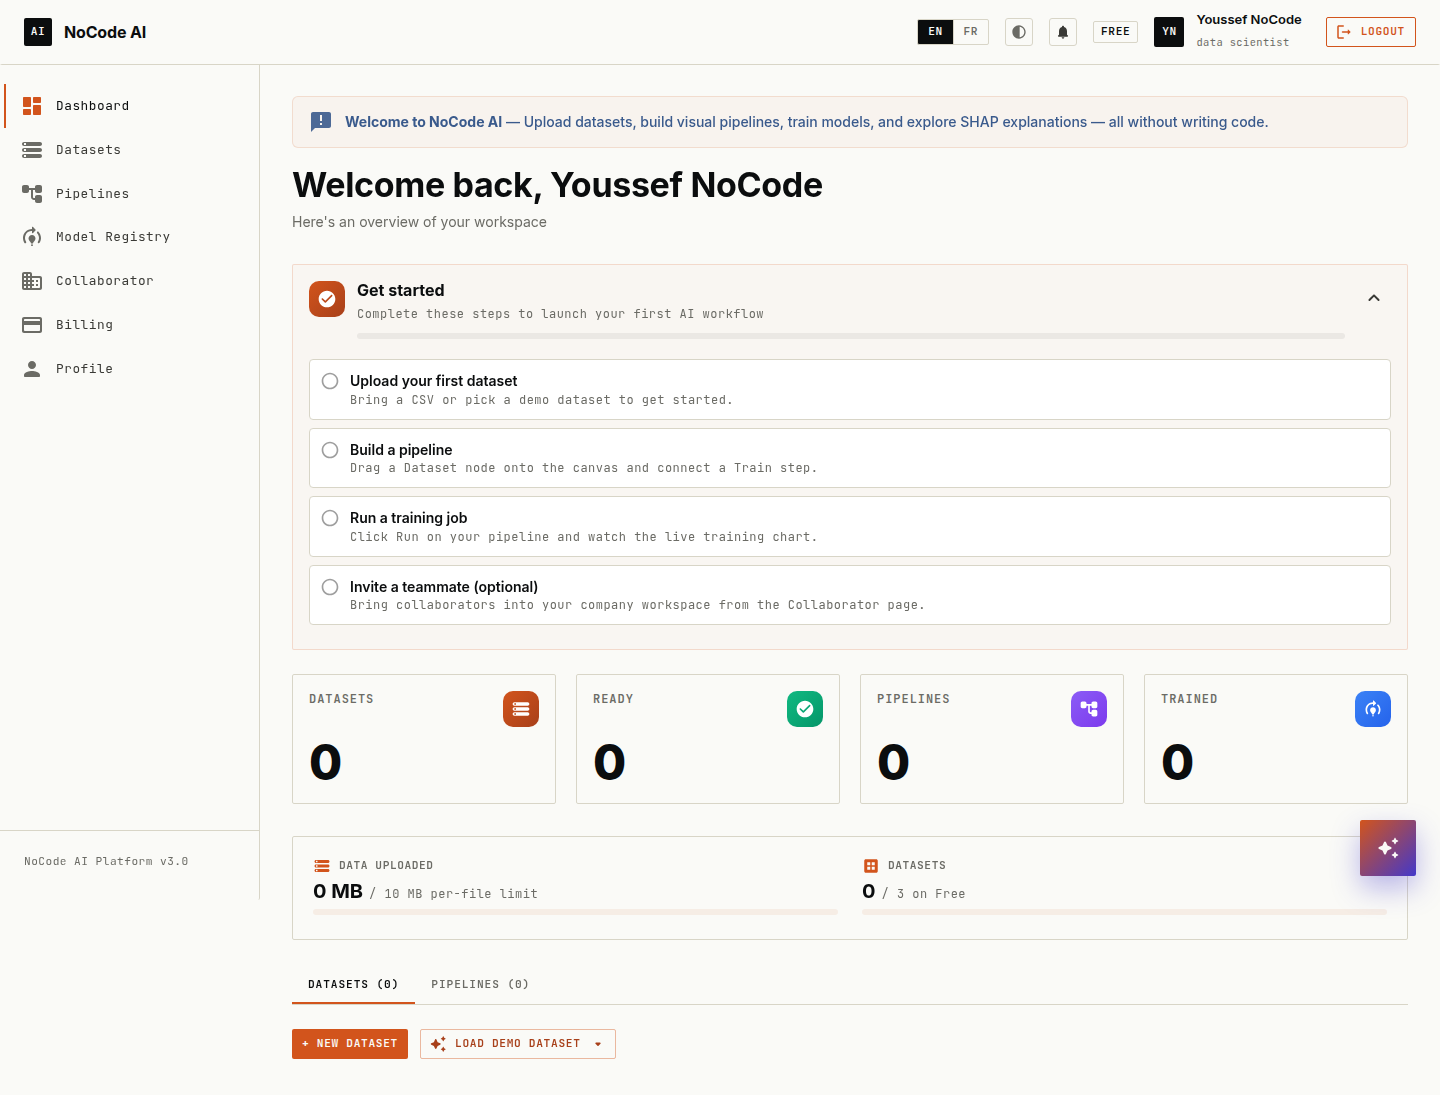
\includegraphics[width=0.85\textwidth, keepaspectratio]{diagrams/ch1_fig4}
  \caption{Home page interface for a signed-in user.}
  \label{fig:ch1_fig4}
\end{figure}

\section{Project Duration}

The project ran across six sprints of roughly two to three weeks each,
with a runnable demo and a self-contained git tag at the end of every
sprint. The Gantt chart in Chapter~3 captures the planned versus
actual timeline.

\section*{Conclusion}

This chapter framed the problem the rest of the report addresses ---
how to make machine learning approachable without surrendering data
sovereignty --- and sketched the platform that emerged in response.
The next chapter reviews the existing landscape and explains why the
question is harder to answer with off-the-shelf tools than first
appears.

% ═════════════════════════════════════════════════════════════════════════════
\chapter{Preliminary Study}
% ═════════════════════════════════════════════════════════════════════════════

\section*{Introduction}

Before describing how the platform was built, we look at why nothing
already on the market quite fits the problem. The no-code ML space
is crowded, but the products in it cluster into families that all
share the same blind spot.

\section{Current Situation}

Three categories of product dominate the space.

\textbf{Cloud-native AutoML platforms} (DataRobot, H2O Driverless~AI,
Azure ML Studio, Google Vertex~AI) are polished, exhaustive in their
algorithm catalogues, and almost invariably SaaS-only. Their privacy
story ends at ``trust our infrastructure''. For commercial buyers
without regulatory exposure that may be acceptable; for the regulated
audience this project targets it is not.

\textbf{Open-source notebooks} (Jupyter, Google Colab, DataLab) are
powerful for experts. Every workflow eventually bottoms out in raw
Python --- which is exactly the friction the no-code category was
invented to remove. A domain expert who can read a confusion matrix
but cannot write \texttt{from sklearn.ensemble import
RandomForestClassifier} hits a wall on line one of the first cell.

\textbf{Visual ETL tools} (KNIME, Alteryx, RapidMiner) come closest
in spirit. Their centre of gravity is data preparation rather than
model training, and their LLM panels almost always route requests
back through OpenAI. The locality story they tell only holds for the
tabular path.

\begin{figure}[H]
  \centering
  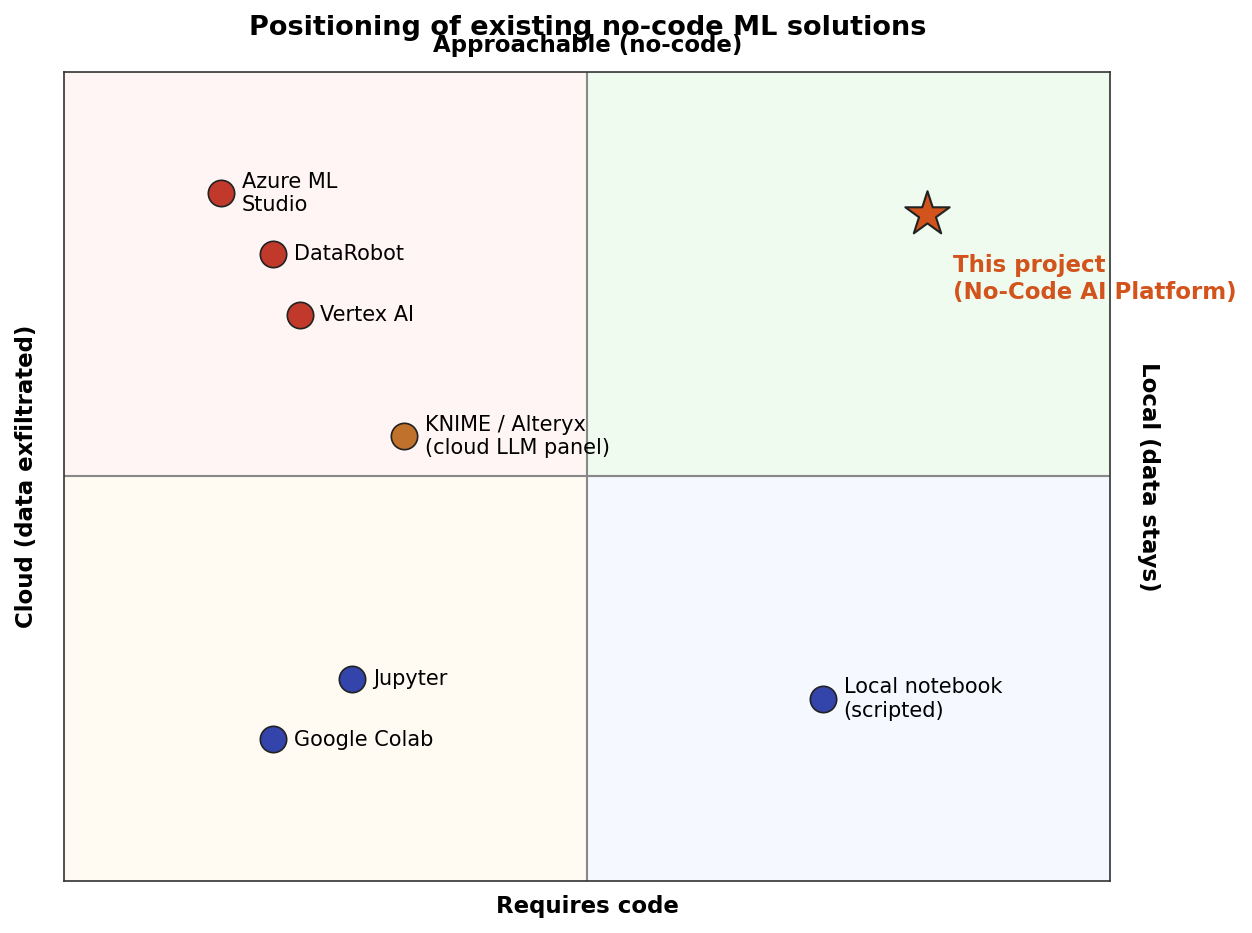
\includegraphics[width=0.85\textwidth, keepaspectratio]{diagrams/ch2_fig1}
  \caption{Positioning of existing no-code ML solutions against this project's design intent.}
  \label{fig:ch2_fig1}
\end{figure}

\section{Observed Problems}

\subsection{Forced data exfiltration}

A clinician analysing patient records, or a bank analyst classifying
transactions, cannot lawfully upload that data to a vendor bucket.
The problem is regulatory, not contractual --- GDPR, HIPAA, and
country-specific banking rules forbid the upload entirely. Every
SaaS AutoML platform listed above assumes the user is fine with that
upload. The audience this project targets is not.

\subsection{Cloud LLM dependence in generative-AI tooling}

Visual tools that grew an ``AI'' panel in the last two years almost
always route the request through OpenAI or a similar API. The panel
is bolted on, not local. For a buyer who cannot ship the prompt
either, the panel is unusable. Worse, those tools rarely document
that the user's prompts are now training data for the vendor.

\subsection{The notebook cliff}

Notebooks solve the locality problem cleanly. They fail on the
no-code one. A non-programmer can drive a Jupyter cell only as far
as someone else has prewritten the code for them, and at that point
the notebook is no longer a notebook but a brittle web form. Closing
this gap is the entire reason a visual canvas exists.

\subsection{Hardware ambiguity}

The few self-hostable products that do exist (KubeFlow, MLflow on
local Kubernetes) assume the operator has a Kubernetes cluster
sitting around. That is not the operating environment of a small
team that has a workstation and an ambition. A platform whose
deployment story requires cluster administration is not really a
self-hostable product; it is a hosted product that pretends.

\section{Objectives of the New System}

The platform sets out to satisfy four objectives at once.

\textbf{Locality.} Every model server, vector store, queue, and
database runs inside the same Docker Compose stack on the user's own
machine.

\textbf{Coverage.} Three workloads --- tabular ML, RAG-style
generative AI, and image classification --- share the same canvas.
The user does not need a different product for each.

\textbf{Approachability.} A canvas-based UI that a non-programmer can
drive end to end, with per-node validation that catches the obvious
mistakes (a Train node with no upstream Dataset, an Evaluate node
with no completed run) before they reach the worker.

\textbf{Honest hardware story.} The reference deployment is a laptop
with $16$\,GB of RAM and a GTX~1660~Super (6\,GB VRAM). The platform
must run on it, not just compile on it.

Two technical shifts make the fourth objective realistic today and
would not have made it realistic two years ago. Aggressive LLM
quantisation has collapsed model footprints. A three-billion-parameter
model in FP16 occupies roughly $12$\,GB of weights; the
\texttt{Q4\_K\_M} four-bit quantisation shrinks that to about
$2$\,GB, while preserving most of the original quality on
conversational tasks. The other shift is first-class GPU inference
runtimes for consumer hardware. Ollama, llama.cpp, and vLLM all
expose efficient batched inference on cards with $4$--$8$\,GB of
VRAM. A 1660 Super, with $6$\,GB of VRAM and $30$\,TFLOPS of FP16
throughput, serves roughly $30$ tokens per second on a 3B model ---
enough latency budget for an interactive RAG chat.

\begin{figure}[H]
  \centering
  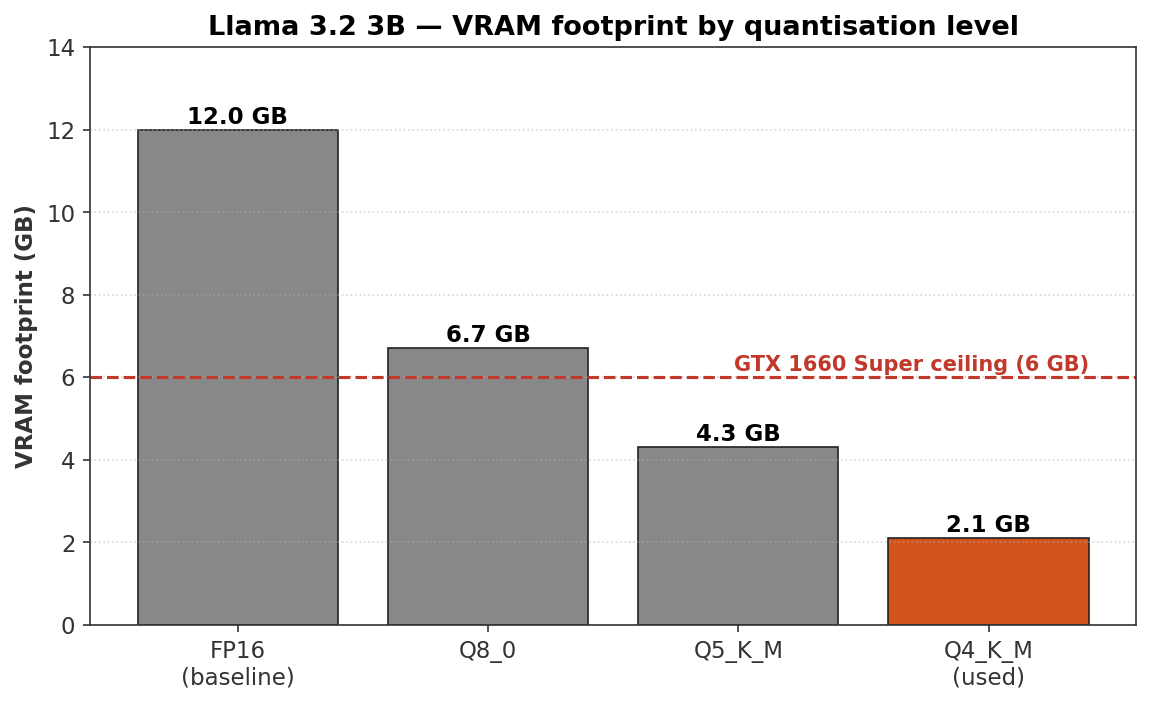
\includegraphics[width=0.85\textwidth, keepaspectratio]{diagrams/ch2_fig2}
  \caption{Quantisation level versus VRAM footprint for a 3B-parameter model.}
  \label{fig:ch2_fig2}
\end{figure}

\section{État de l'art technique}

The platform builds on four well-documented technique families. We
summarise the relevant prior art here so the sprint chapters can
reference it without restating the basics.

\textbf{Tree-based gradient boosting.} XGBoost~\cite{xgboost} formalised
regularised gradient boosting on decision trees and remains the
default for tabular ML competitions. The Tunisian DSI thesis context
favours XGBoost over deep tabular models because its training cost
fits in minutes on a CPU and its hyperparameter surface is mature.

\textbf{Post-hoc explainability via Shapley values.} The SHAP
framework~\cite{shap} attributes a model's output to its input
features using Shapley values from cooperative game theory. The
optimised TreeExplainer variant lifts the cost of SHAP from
prohibitive to interactive on tree models --- the only reason SHAP is a
live feature in this platform rather than a batch job.

\textbf{Retrieval-Augmented Generation.} Lewis et al.~\cite{rag}
introduced the RAG formulation: embed query and corpus, retrieve top-k
chunks by similarity, condition a generative model on the retrieved
context. This formulation is what makes a local LLM useful on private
documents --- the model is small (3B), the corpus does the heavy
lifting.

\textbf{Compact CNN architectures.} Three architecture families are
represented: LeNet~\cite{lenet} as a smoke-test baseline, residual
networks~\cite{resnet} as the workhorse, and
MobileNetV3~\cite{mobilenetv3} as the transfer-learning option. Each
sits at a different parameter/accuracy operating point compatible with
the 6\,GB VRAM budget.

\section*{Conclusion}

Cloud platforms solve the wrong half of the problem, notebooks demand
too much of the user, and visual ETL tools are not aimed at model
training. The platform described in the rest of this report fills
that gap deliberately: local by construction, broad enough to cover
the three AI workloads that matter today, and modest enough in its
hardware appetite to run on a laptop.

% ═════════════════════════════════════════════════════════════════════════════
\chapter{Methodology and Working Environment}
% ═════════════════════════════════════════════════════════════════════════════

\section*{Introduction}

Six sprints, one team, three AI workloads on a single GPU --- the
project's primary risk was scope, not technique. This chapter
explains the methodology used to keep that risk in check, the
toolchain that anchored the build, and the layout of the services
those choices produced.

\section{Comparison of Project Management Methodologies}

Three styles were considered before settling on one. Table
\ref{tab:methodology_comparison} captures the trade-offs against the
constraints of an ML-heavy solo project.

\begin{table}[H]
\centering
\caption{Comparison of candidate project management methodologies.}
\label{tab:methodology_comparison}
\begin{tabular}{@{}p{0.18\linewidth} L{0.36\linewidth} L{0.36\linewidth}@{}}
\toprule
\textbf{Approach} & \textbf{Strengths} & \textbf{Why rejected (or chosen)} \\
\midrule
Waterfall & Predictable cost, single up-front spec, easy to communicate. & Fails an ML project where the cost of a feature is genuinely unpredictable --- Prophet's CmdStan dependency alone pushed a ``trivial'' algorithm into half a sprint. \textbf{Rejected.} \\
Pure Kanban & Continuous flow, no ceremony overhead. & Removes the dated checkpoints needed to demo to a supervisor; produces no natural fallback point if a late feature fails. \textbf{Rejected.} \\
Scrum-lite & Short fixed-length sprints, runnable demo + git tag at each boundary, written retro. & Enough ceremony to enforce scope discipline without consuming the sprint. \textbf{Chosen.} \\
\bottomrule
\end{tabular}
\end{table}

\textbf{Waterfall} plans everything upfront, builds in order, and
demos at the end. That shape fails an ML project where the cost of a
feature is genuinely unpredictable. \textbf{Pure Kanban} offers
continuous flow with no sprint boundary, which removes exactly the
checkpoints needed to demo to a supervisor on a fixed cadence.
\textbf{Scrum-lite}, the chosen approach, runs short sprints with a
runnable demo, a self-contained git tag, and a retrospective note at
each boundary --- enough ceremony to enforce scope discipline
without consuming the sprint.

\section{The Choice of Agile Methodology}

Two reasons pushed the project toward Agile. First, ML capacity
planning is unpredictable. A feature that looks easy on paper hides
compile-from-source dependencies, missing CUDA wheels, or libraries
whose API has shifted between minor versions. Agile's sprint boundary
absorbs that kind of slip. Second, the project needed dated
checkpoints with no hand-waving. Without sprint structure the
deliverable becomes a single ``everything works at once'' release,
with no story to tell along the way and no fallback when a late
feature falls through.

\section{Scrum Methodology}

\begin{figure}[H]
  \centering
  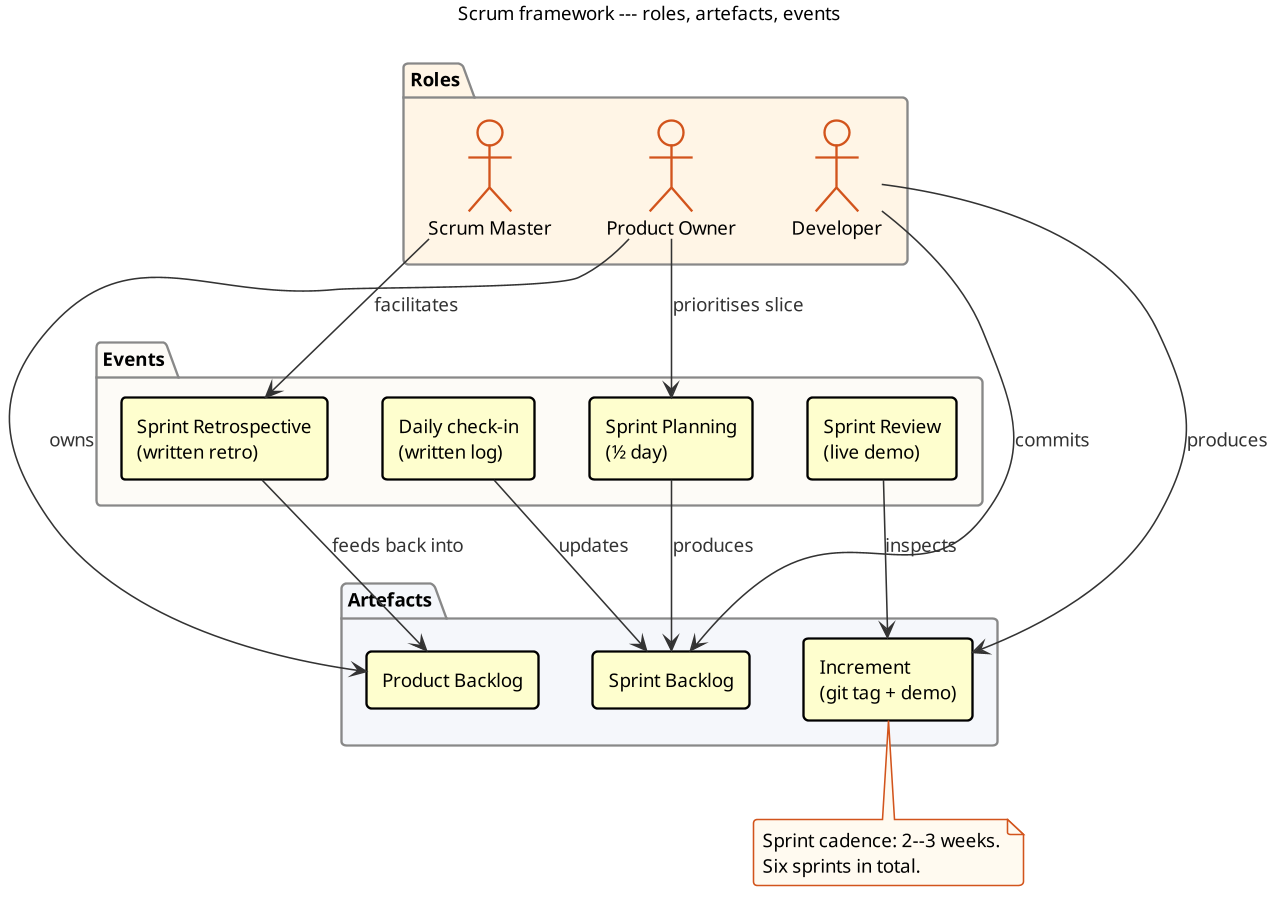
\includegraphics[width=0.85\textwidth, keepaspectratio]{diagrams/ch3_fig1}
  \caption{The Scrum framework --- roles, artefacts, events.}
  \label{fig:ch3_fig1}
\end{figure}

\subsection{Scrum Roles}

In a small team the roles collapse onto a single person at a time.
What does not collapse is the discipline of switching hats. When
planning, the operator is the Product Owner --- writing user stories
and prioritising the backlog. When building, the operator is the
Developer. When reviewing the sprint, the operator becomes the Scrum
Master --- asking what went wrong, what would change next time.
Treating those as three roles, even when they share one head, keeps
the practice honest.

\subsection{Scrum Artefacts}

\begin{itemize}
    \item \textbf{Product Backlog.} A single Markdown file under
        \texttt{docs/backlog.md}, grouped by sprint.
    \item \textbf{Sprint Backlog.} The slice of the product backlog
        promised for the current sprint, lifted into the sprint's
        section.
    \item \textbf{Increment.} The git tag at the end of the sprint,
        plus the demo recording.
\end{itemize}

\subsection{Scrum Events}

\begin{itemize}
    \item \textbf{Sprint Planning.} Half a day at the start of each
        sprint. Carry-over from the previous sprint plus a fresh
        slice of the backlog.
    \item \textbf{Daily check-in.} A short written log entry, not a
        meeting.
    \item \textbf{Sprint Review.} A live demo with the supervisor at
        sprint end.
    \item \textbf{Sprint Retrospective.} A retro note in the same
        Markdown backlog, under the sprint heading.
\end{itemize}

\section{Product Backlog}

Six sprints, each closing with a runnable demo and a self-contained
git tag:

\begin{itemize}
    \item \textbf{Sprint~1 --- Authentication, Gateway, Data
        Ingestion.} Foundational service mesh.
    \item \textbf{Sprint~2 --- Visual Pipeline Editor and Tabular
        ML.} Canvas, fourteen algorithms, SHAP, model export.
    \item \textbf{Sprint~3 --- Local Generative AI and RAG.} Ollama,
        \texttt{pgvector}, streamed chat.
    \item \textbf{Sprint~4 --- Deep Learning for Image
        Classification.} PyTorch service, three CNNs, the VRAM
        guard.
    \item \textbf{Sprint~5 --- Multi-tenancy and Real-Time
        Collaboration.} Project ACL, cursors, threaded chat, Meet
        links.
    \item \textbf{Sprint~6 --- Dashboard, i18n, Accessibility, Admin
        Console.} Operability and polish.
\end{itemize}

The three AI workloads sit back-to-back as Sprints~2--4. That order
matters: tabular ML grounds the canvas and the algorithm-registry
abstraction; RAG extends both into streaming chat; deep learning then
reuses the canvas, the registry, and the live-training channel
without rebuilding any of them.

\section{Project Planning}

\begin{landscape}
\begin{figure}[H]
  \centering
  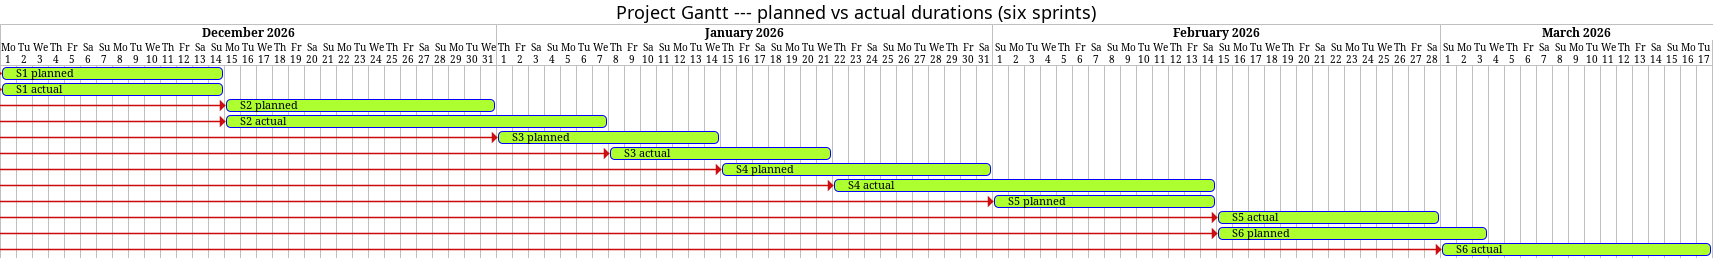
\includegraphics[width=0.95\linewidth, keepaspectratio]{diagrams/ch3_fig2}
  \caption{Gantt chart --- planned versus actual duration for the six-sprint plan.}
  \label{fig:ch3_fig2}
\end{figure}
\end{landscape}

Two sprints slipped by roughly a week each. Sprint~2 ran long because
the live training visualisation had a Plotly autoscale bug that took
a day to diagnose --- progress percentage and metric values lived on
incompatible Y-axis ranges. Sprint~4 ran long because the static VRAM
estimate needed an empirical recalibration pass after the first real
GPU run exceeded the predicted budget by roughly $15\%$ on
MobileNet-V3 at 224\,px batch~32.

\section{Technologies}

\textbf{Frontend --- React~18 + Vite + TypeScript + MUI.} React for
the ecosystem, Vite because cold starts under
\texttt{create-react-app} were unworkable, MUI because it ships
accessible components that already satisfy WCAG~AA without bespoke
work.

\textbf{Backend --- Flask + Celery + Flask-SocketIO.} Flask was the
lowest-common-denominator choice for a microservice. FastAPI would
have given typed routes for free, but every template used as a
starting point assumed Flask, and rewriting five services for typing
was not a fight worth picking. Celery handles every CPU-bound task ---
profiling, preprocessing, H2O training, RAG ingestion, image
extraction, and PyTorch training all live on their own queue.

\textbf{Postgres + pgvector for relational and vector data.}
Co-locating the vector store with the auth schema avoided a sixth
backing service. \texttt{pgvector}'s IVFFlat index is more than
enough for the few hundred thousand chunks a single-tenant local
deployment is ever likely to hold.

\textbf{MongoDB for everything schemaless.} Datasets, pipelines,
model versions, task results --- anything whose shape evolves
between sprints lives in Mongo. A Postgres JSONB column was
considered for this and rejected: lossless storage, flexible queries,
and zero migrations as new statistics get added all favoured Mongo.

\textbf{Redis for queue + cache + socket message bus.} Three logical
databases on the same instance --- DB~0 for Celery, DB~1 for Celery
results, DB~2 for the SocketIO message queue.

\textbf{Ollama for local LLM inference.} The alternative was calling
\texttt{llama.cpp} directly, which would have meant building an HTTP
shim around it. Ollama's REST API is mature enough that the trade
wasn't close.

\textbf{PyTorch + torchvision for image classification.} CUDA~12.1
wheels are downloaded from PyTorch's index inside the Dockerfile so
the host only needs the NVIDIA driver plus
\texttt{nvidia-container-toolkit}.

\section{Architecture}

\begin{figure}[H]
  \centering
  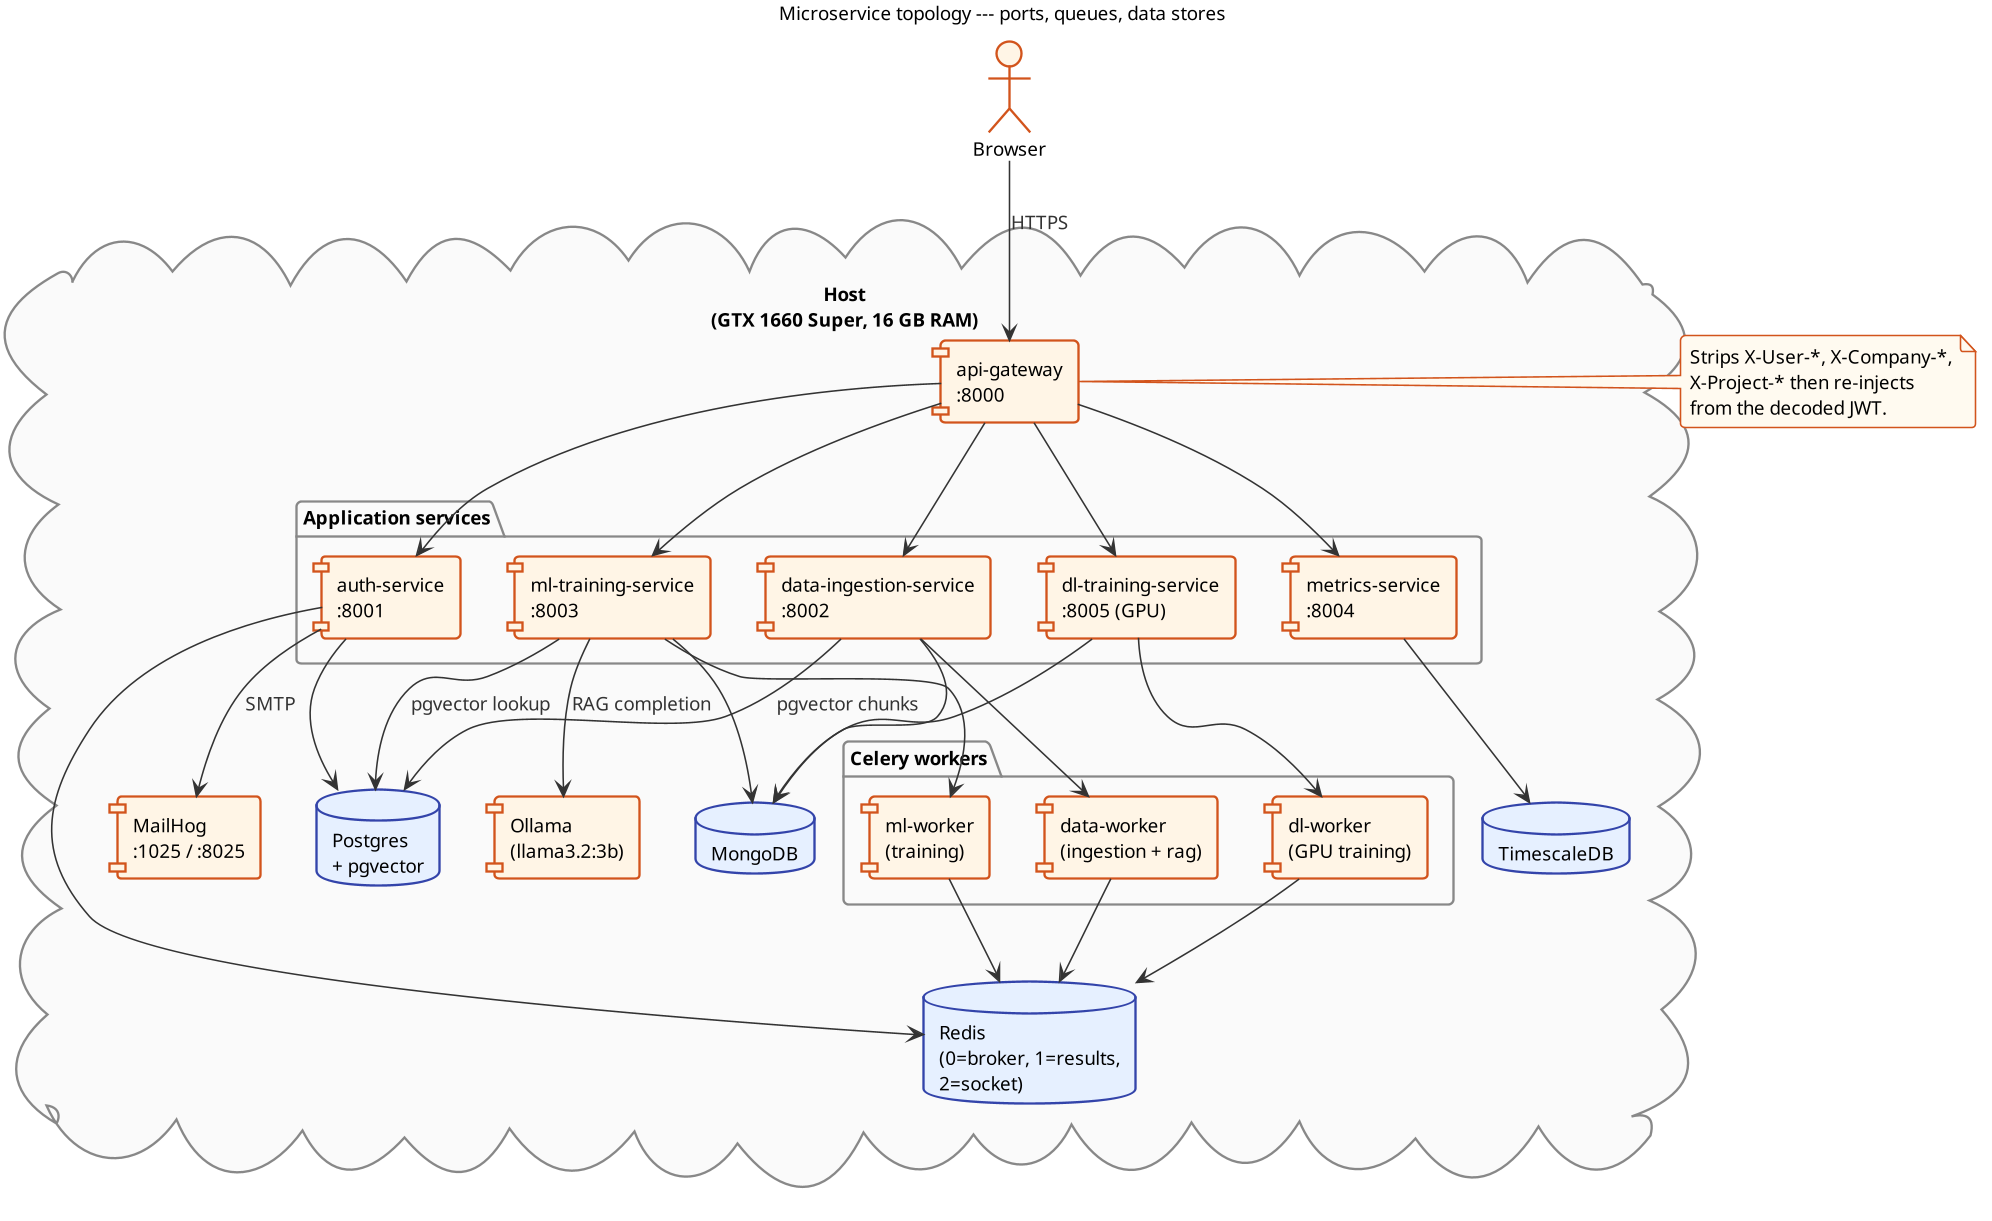
\includegraphics[width=0.85\textwidth, keepaspectratio]{diagrams/ch3_fig3}
  \caption{High-level microservice topology.}
  \label{fig:ch3_fig3}
\end{figure}

\begin{figure}[H]
  \centering
  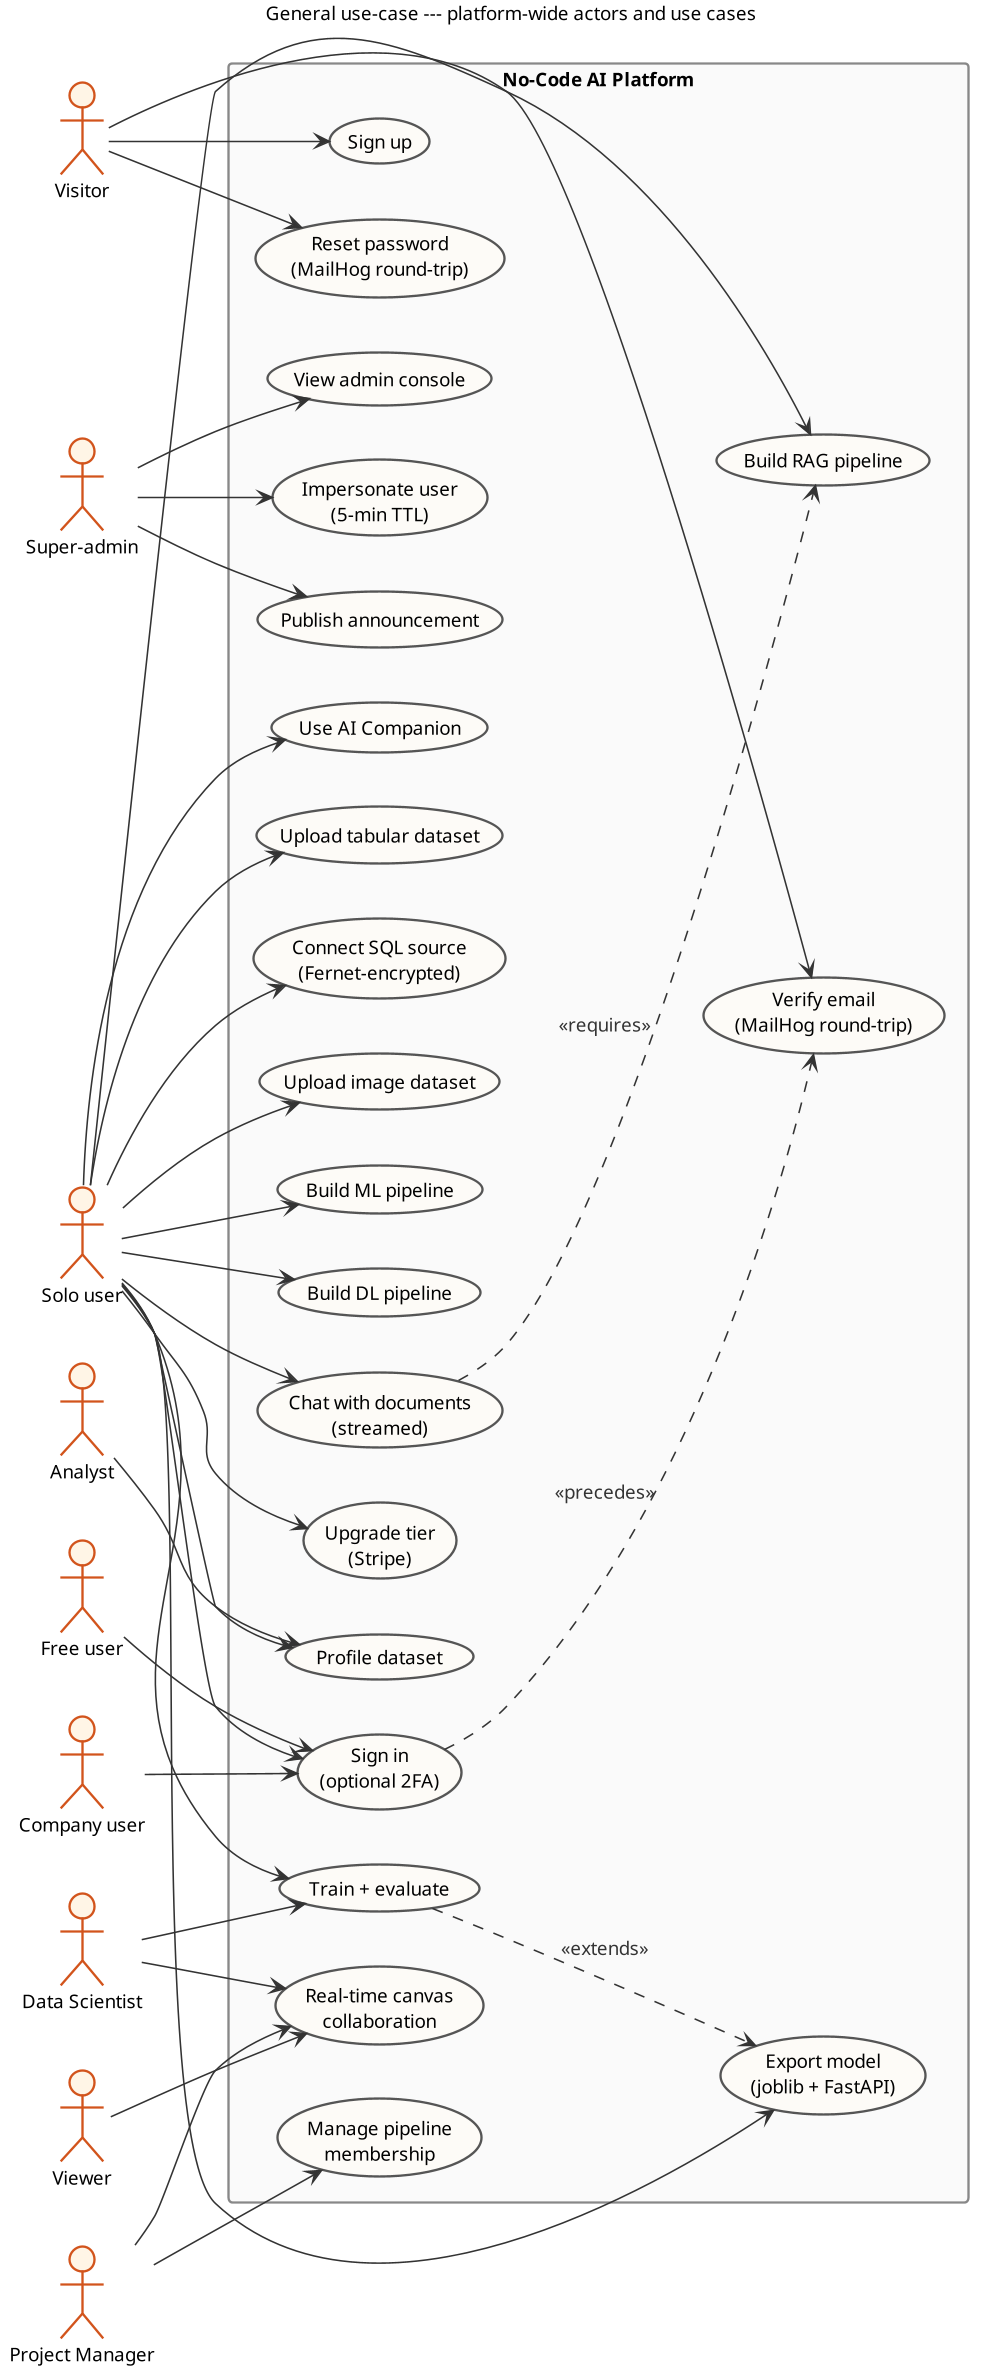
\includegraphics[height=0.9\textheight, keepaspectratio]{diagrams/ch3_fig_general_usecase}
  \caption{General use-case diagram --- complete actor / use-case map across the six sprints.}
  \label{fig:ch3_fig_general_usecase}
\end{figure}

\begin{figure}[H]
  \centering
  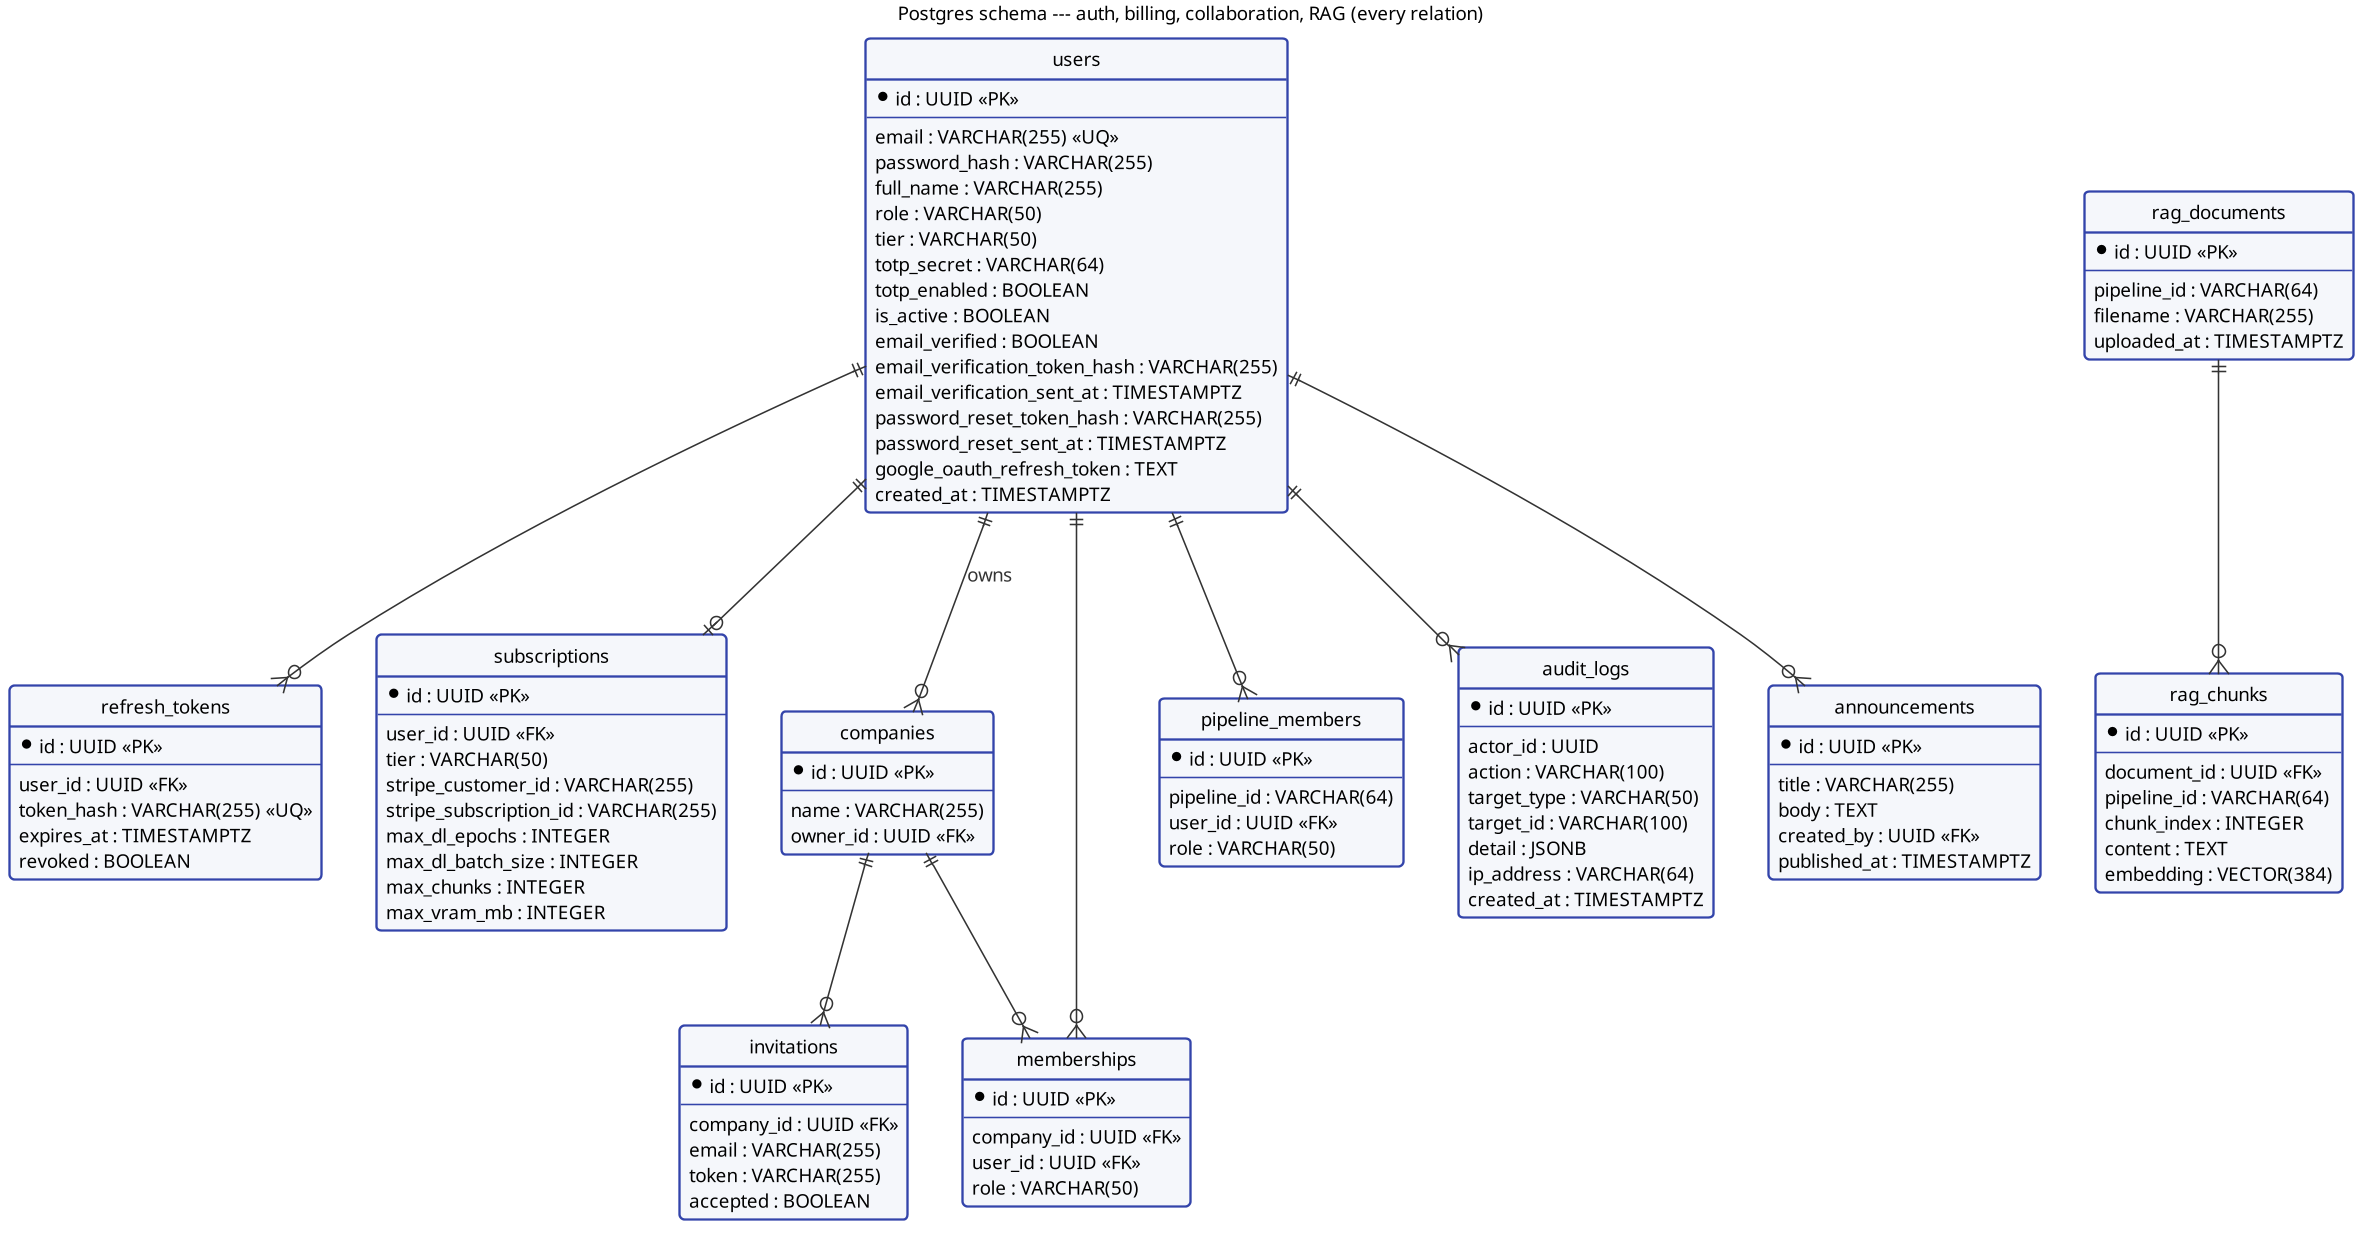
\includegraphics[width=0.95\linewidth]{diagrams/ch3_fig_db_schema}
  \caption{Database schema --- Postgres tables across auth-service, rag, and pipeline collaboration.}
  \label{fig:ch3_fig_db_schema}
\end{figure}

\begin{itemize}
    \item \texttt{api-gateway} (port 8000) --- decodes JWTs, injects
        \texttt{X-User-Id} / \texttt{X-User-Tier} /
        \texttt{X-User-Role} headers, proxies to the upstream
        services. Hosts the SocketIO server for chat and training
        presence.
    \item \texttt{auth-service} (port 8001) --- user accounts,
        billing, admin operations, project and company ACL.
    \item \texttt{data-ingestion-service} (port 8002) --- file
        uploads, SQL and S3 connectors, profiling, preprocessing,
        RAG ingestion, image-dataset extraction.
    \item \texttt{ml-training-service} (port 8003) --- the fourteen
        tabular algorithms, model registry, RAG chat orchestration.
    \item \texttt{metrics-service} (port 8004) --- TimescaleDB-backed
        hardware-telemetry collection.
    \item \texttt{dl-training-service} (port 8005) --- PyTorch image
        classification.
\end{itemize}

A GitHub Actions workflow runs four jobs in parallel on every push:
backend lint (\texttt{black}, \texttt{isort}, \texttt{flake8}),
frontend lint (\texttt{eslint}, \texttt{tsc --noEmit}), backend
tests (Postgres + Mongo + Redis spun up as service containers,
\texttt{pytest} per microservice), and frontend tests
(\texttt{vitest} with coverage upload). End-to-end CI runs in
roughly six minutes for a frontend-only change, nine minutes for a
backend change, and fourteen minutes when both sides move at once.

\section*{Conclusion}

The methodology and toolchain held throughout the six sprints. Some
choices --- Flask in particular --- are ones we would revisit if
starting over, but they shipped a working system without rework. The
next chapter opens the sprint walkthrough.

% ═════════════════════════════════════════════════════════════════════════════
\chapter{Sprint 1: Authentication, Gateway, and Data Ingestion}
% ═════════════════════════════════════════════════════════════════════════════

\section*{Introduction}

Sprint~1 was the foundation sprint. Nothing glamorous --- no
canvases, no models --- but the design choices made in these two
weeks shaped every later sprint. The gateway pattern and the
shared-volume convention introduced here are the quiet load-bearing
decisions of the whole project.

\section{Sprint Backlog}

\begin{table}[H]
\centering
\caption{Sprint~1 backlog --- foundation services.}
\label{tab:sprint1_backlog}
\begin{tabular}{@{}p{0.05\linewidth} L{0.55\linewidth} p{0.1\linewidth} p{0.18\linewidth}@{}}
\toprule
\textbf{ID} & \textbf{User Story / Task} & \textbf{Priority} & \textbf{Estimation (d)} \\
\midrule
US-01 & Stateless JWT authentication with refresh-token rotation. & High & 2 \\
US-02 & Redis-backed token revocation list. & High & 1 \\
US-03 & Role-based access control (super-admin + tenant roles). & High & 1 \\
US-04 & API gateway: strip client-supplied identity headers, inject from decoded JWT. & High & 2 \\
US-05 & Optional TOTP two-factor authentication. & Medium & 1.5 \\
US-06 & Per-IP and per-user rate limiting at the gateway. & Medium & 0.5 \\
US-07 & Email verification on signup via MailHog. & Medium & 1 \\
US-08 & Password reset round-trip via MailHog. & Medium & 1 \\
US-09 & \texttt{data-ingestion-service}: CSV/Excel upload, async profiling. & High & 2 \\
US-10 & SQL connectors (Postgres/MySQL) with Fernet-encrypted credentials. & Medium & 1.5 \\
US-11 & Mongo-backed dataset metadata + Parquet preprocessing output. & High & 1.5 \\
\bottomrule
\end{tabular}
\end{table}

\subsection{Use case --- Sign in with optional 2FA}

\begin{table}[H]
\centering
\caption{Textual description of the ``Sign in with optional 2FA'' use case.}
\label{tab:uc_signin}
\begin{tabular}{@{}p{0.22\linewidth} L{0.7\linewidth}@{}}
\toprule
\textbf{Field} & \textbf{Value} \\
\midrule
Use case & Sign in with optional 2FA \\
Primary actor & End user (any tier) \\
Pre-conditions & Account exists and \texttt{email\_verified = true}. \\
Trigger & User submits the Sign In form with email + password. \\
Nominal scenario & (1) Gateway forwards \texttt{POST /auth/login}.
(2) Auth-service validates credentials with bcrypt.
(3) If \texttt{totp\_enabled = false}, issue access + refresh tokens.
(4) Frontend persists access token in \texttt{sessionStorage}, sets HttpOnly refresh cookie.
(5) Redirect to \texttt{/dashboard}. \\
Alt. scenario A & Credentials invalid $\to$ 401 + audit event \texttt{auth.login\_failed}. \\
Alt. scenario B & \texttt{email\_verified = false} $\to$ 403 with link hint to MailHog. \\
Alt. scenario C & \texttt{totp\_enabled = true} $\to$ 200 \texttt{requires\_2fa} + 5-min session token; user enters 6-digit code on \texttt{/2fa}. \\
Post-conditions & Refresh token JTI persisted; previous JTI blacklisted on next rotation. \\
\bottomrule
\end{tabular}
\end{table}

\subsection{Use case --- Verify email via MailHog}

\begin{table}[H]
\centering
\caption{Textual description of the ``Verify email'' use case.}
\label{tab:uc_verify}
\begin{tabular}{@{}p{0.22\linewidth} L{0.7\linewidth}@{}}
\toprule
\textbf{Field} & \textbf{Value} \\
\midrule
Use case & Verify email via MailHog \\
Primary actor & Newly registered user \\
Pre-conditions & \texttt{POST /auth/register} completed; token persisted as SHA-256 hash with 24-hour TTL. \\
Trigger & User clicks the link inside the verification email. \\
Nominal scenario & (1) Browser hits \texttt{/verify-email?token=…}.
(2) Frontend posts the token to \texttt{POST /auth/verify-email}.
(3) Auth-service matches \texttt{sha256(token)} against \texttt{users.email\_verification\_token\_hash}.
(4) Sets \texttt{email\_verified = true}; clears the token row.
(5) Frontend shows success card with a continue-to-sign-in button. \\
Alt. scenario A & Token expired ($\geq$ 24h) $\to$ 400 \texttt{invalid\_or\_expired\_token}; user can request a fresh mail. \\
Alt. scenario B & Token reused $\to$ 400; the token hash is cleared on first success. \\
Post-conditions & Account is now eligible for sign-in. \\
\bottomrule
\end{tabular}
\end{table}

\section{Design}

\begin{figure}[H]
  \centering
  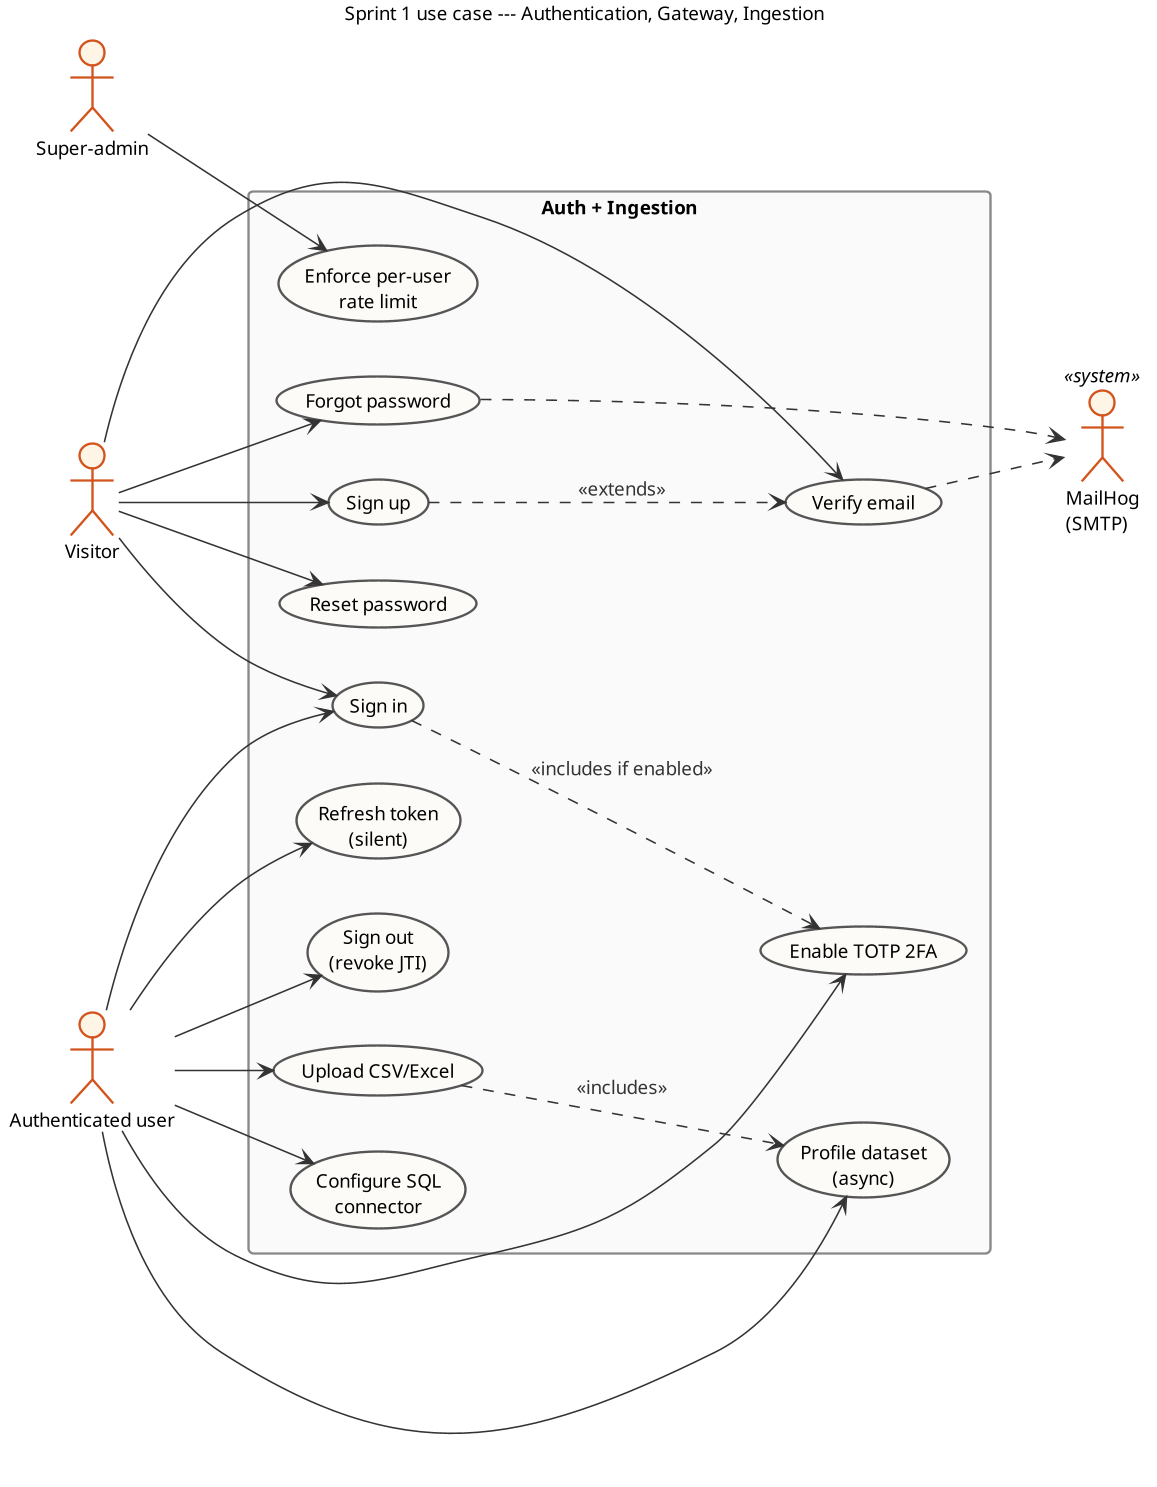
\includegraphics[width=0.85\textwidth, keepaspectratio]{diagrams/ch4_fig1}
  \caption{Use case diagram --- authentication and ingestion.}
  \label{fig:ch4_fig1}
\end{figure}

\begin{figure}[H]
  \centering
  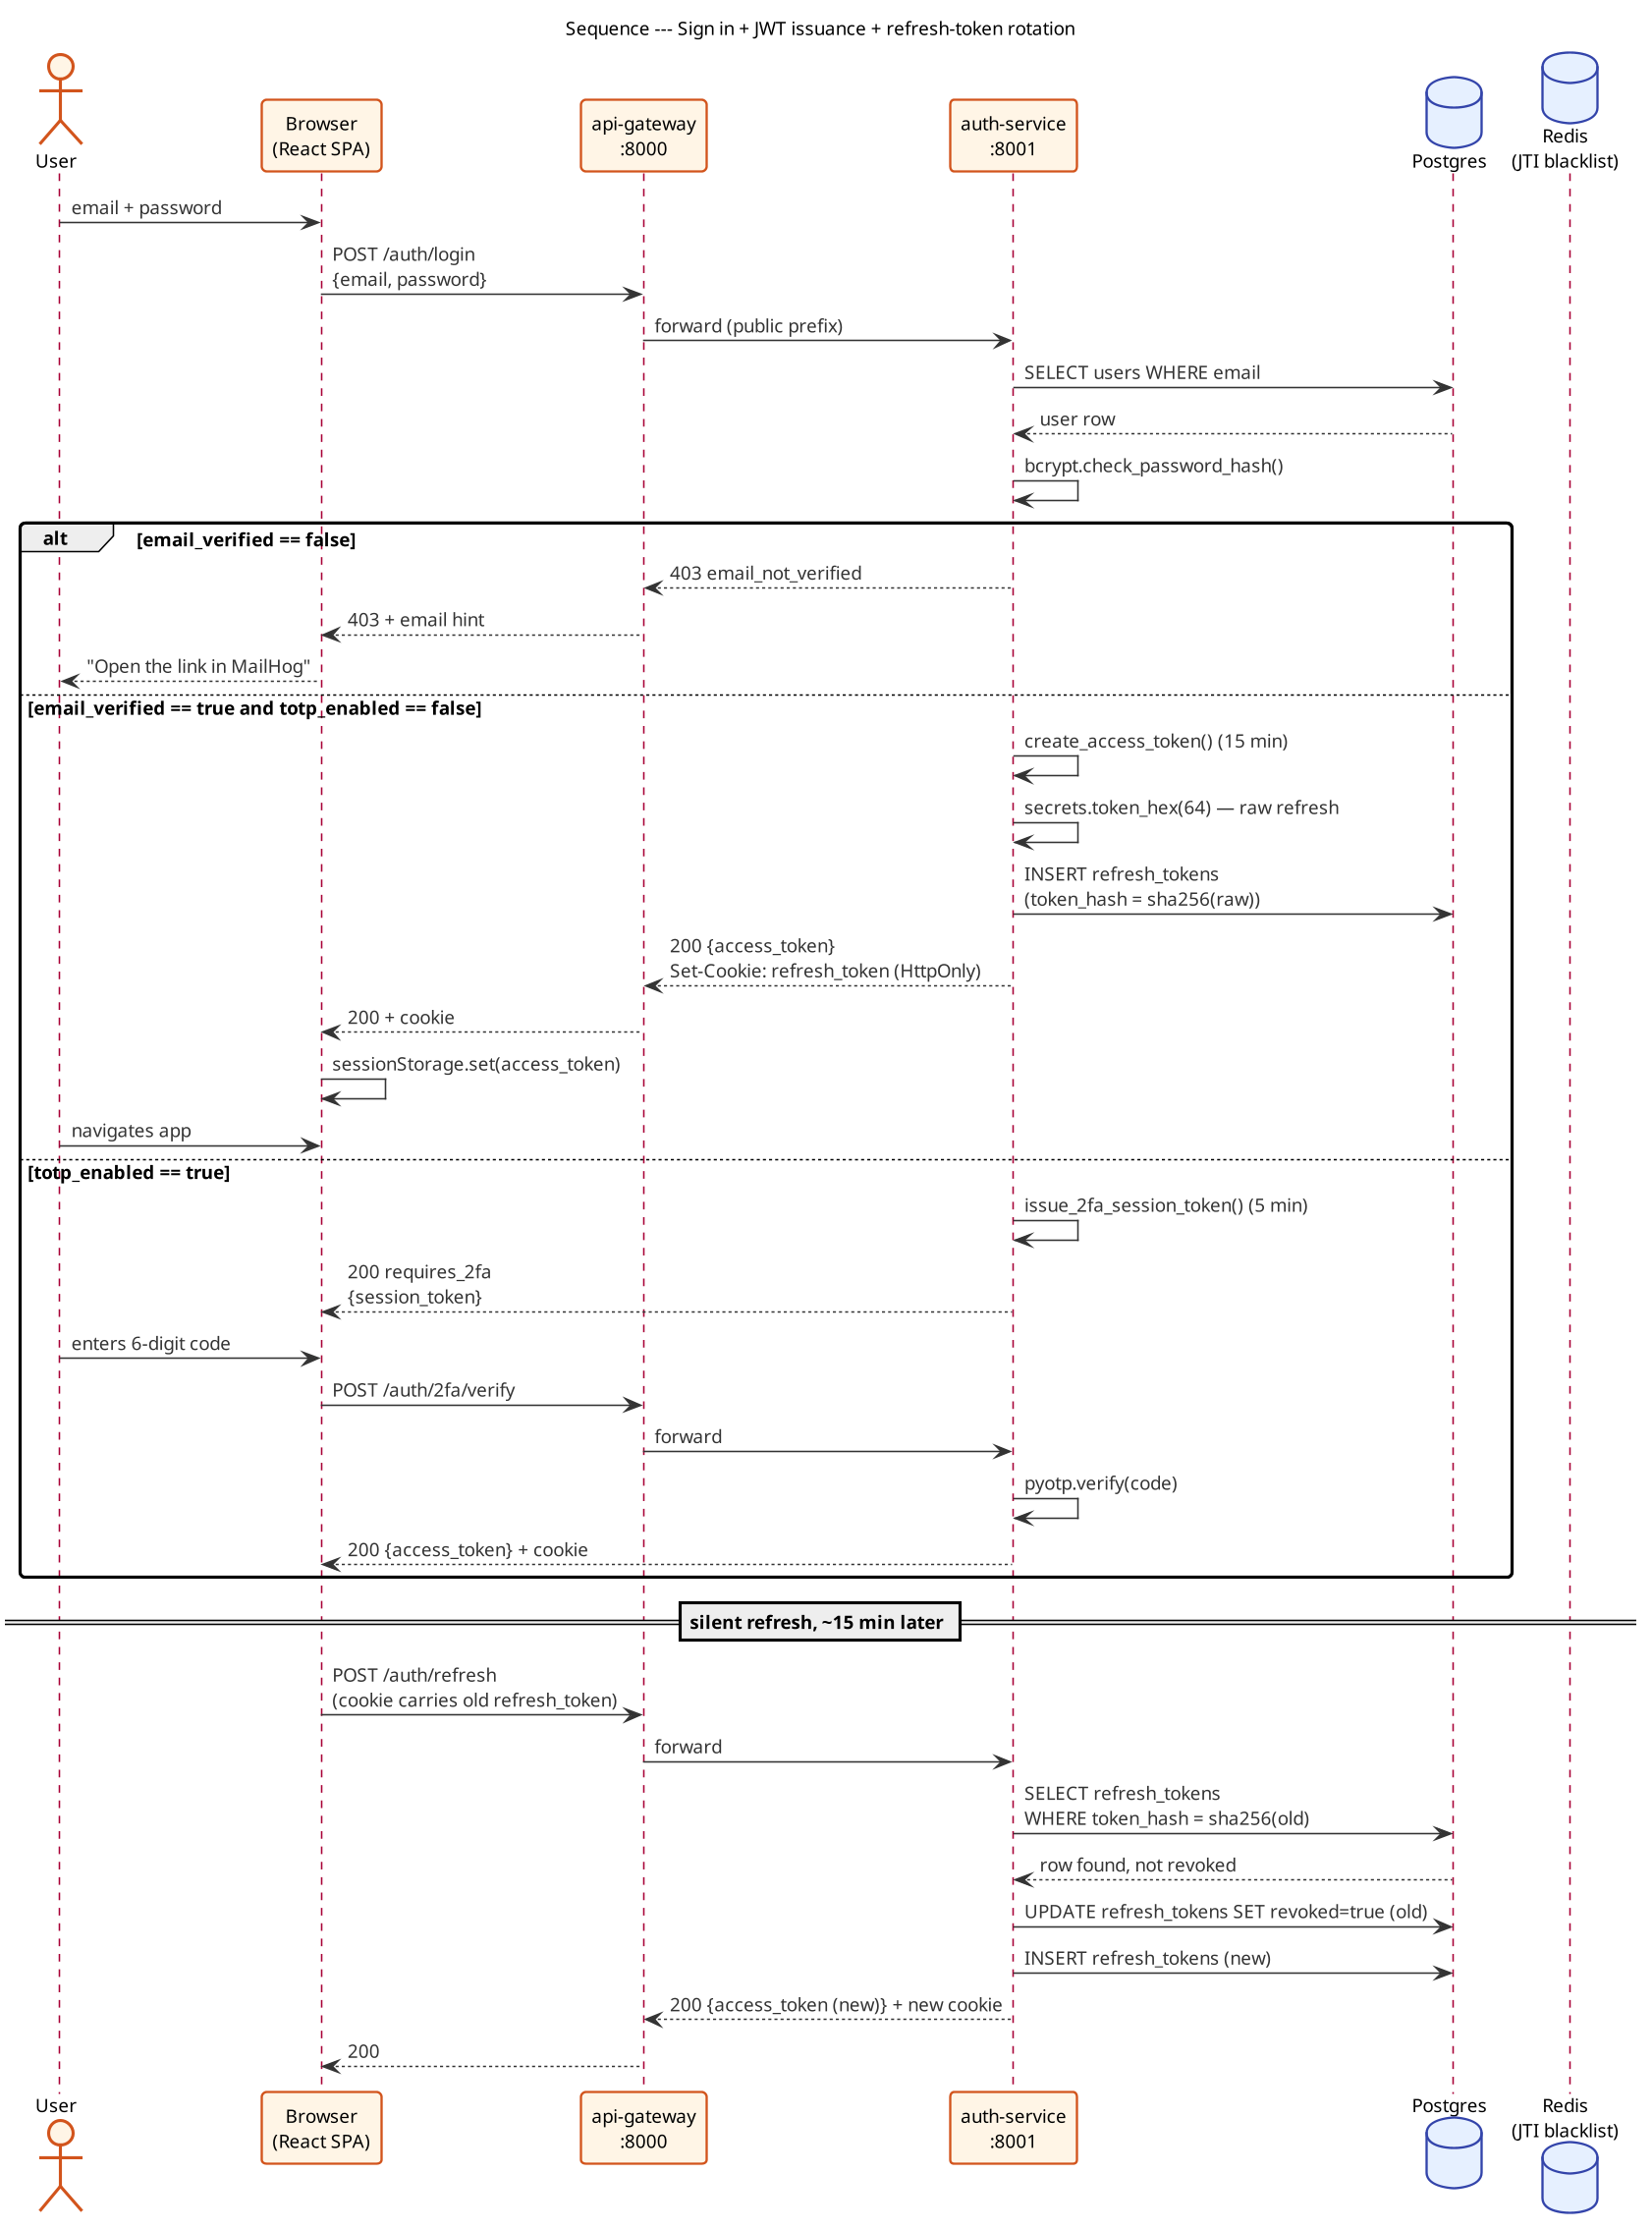
\includegraphics[width=0.85\textwidth, keepaspectratio]{diagrams/ch4_fig2}
  \caption{Sequence diagram --- login plus refresh-token rotation.}
  \label{fig:ch4_fig2}
\end{figure}

\begin{figure}[H]
  \centering
  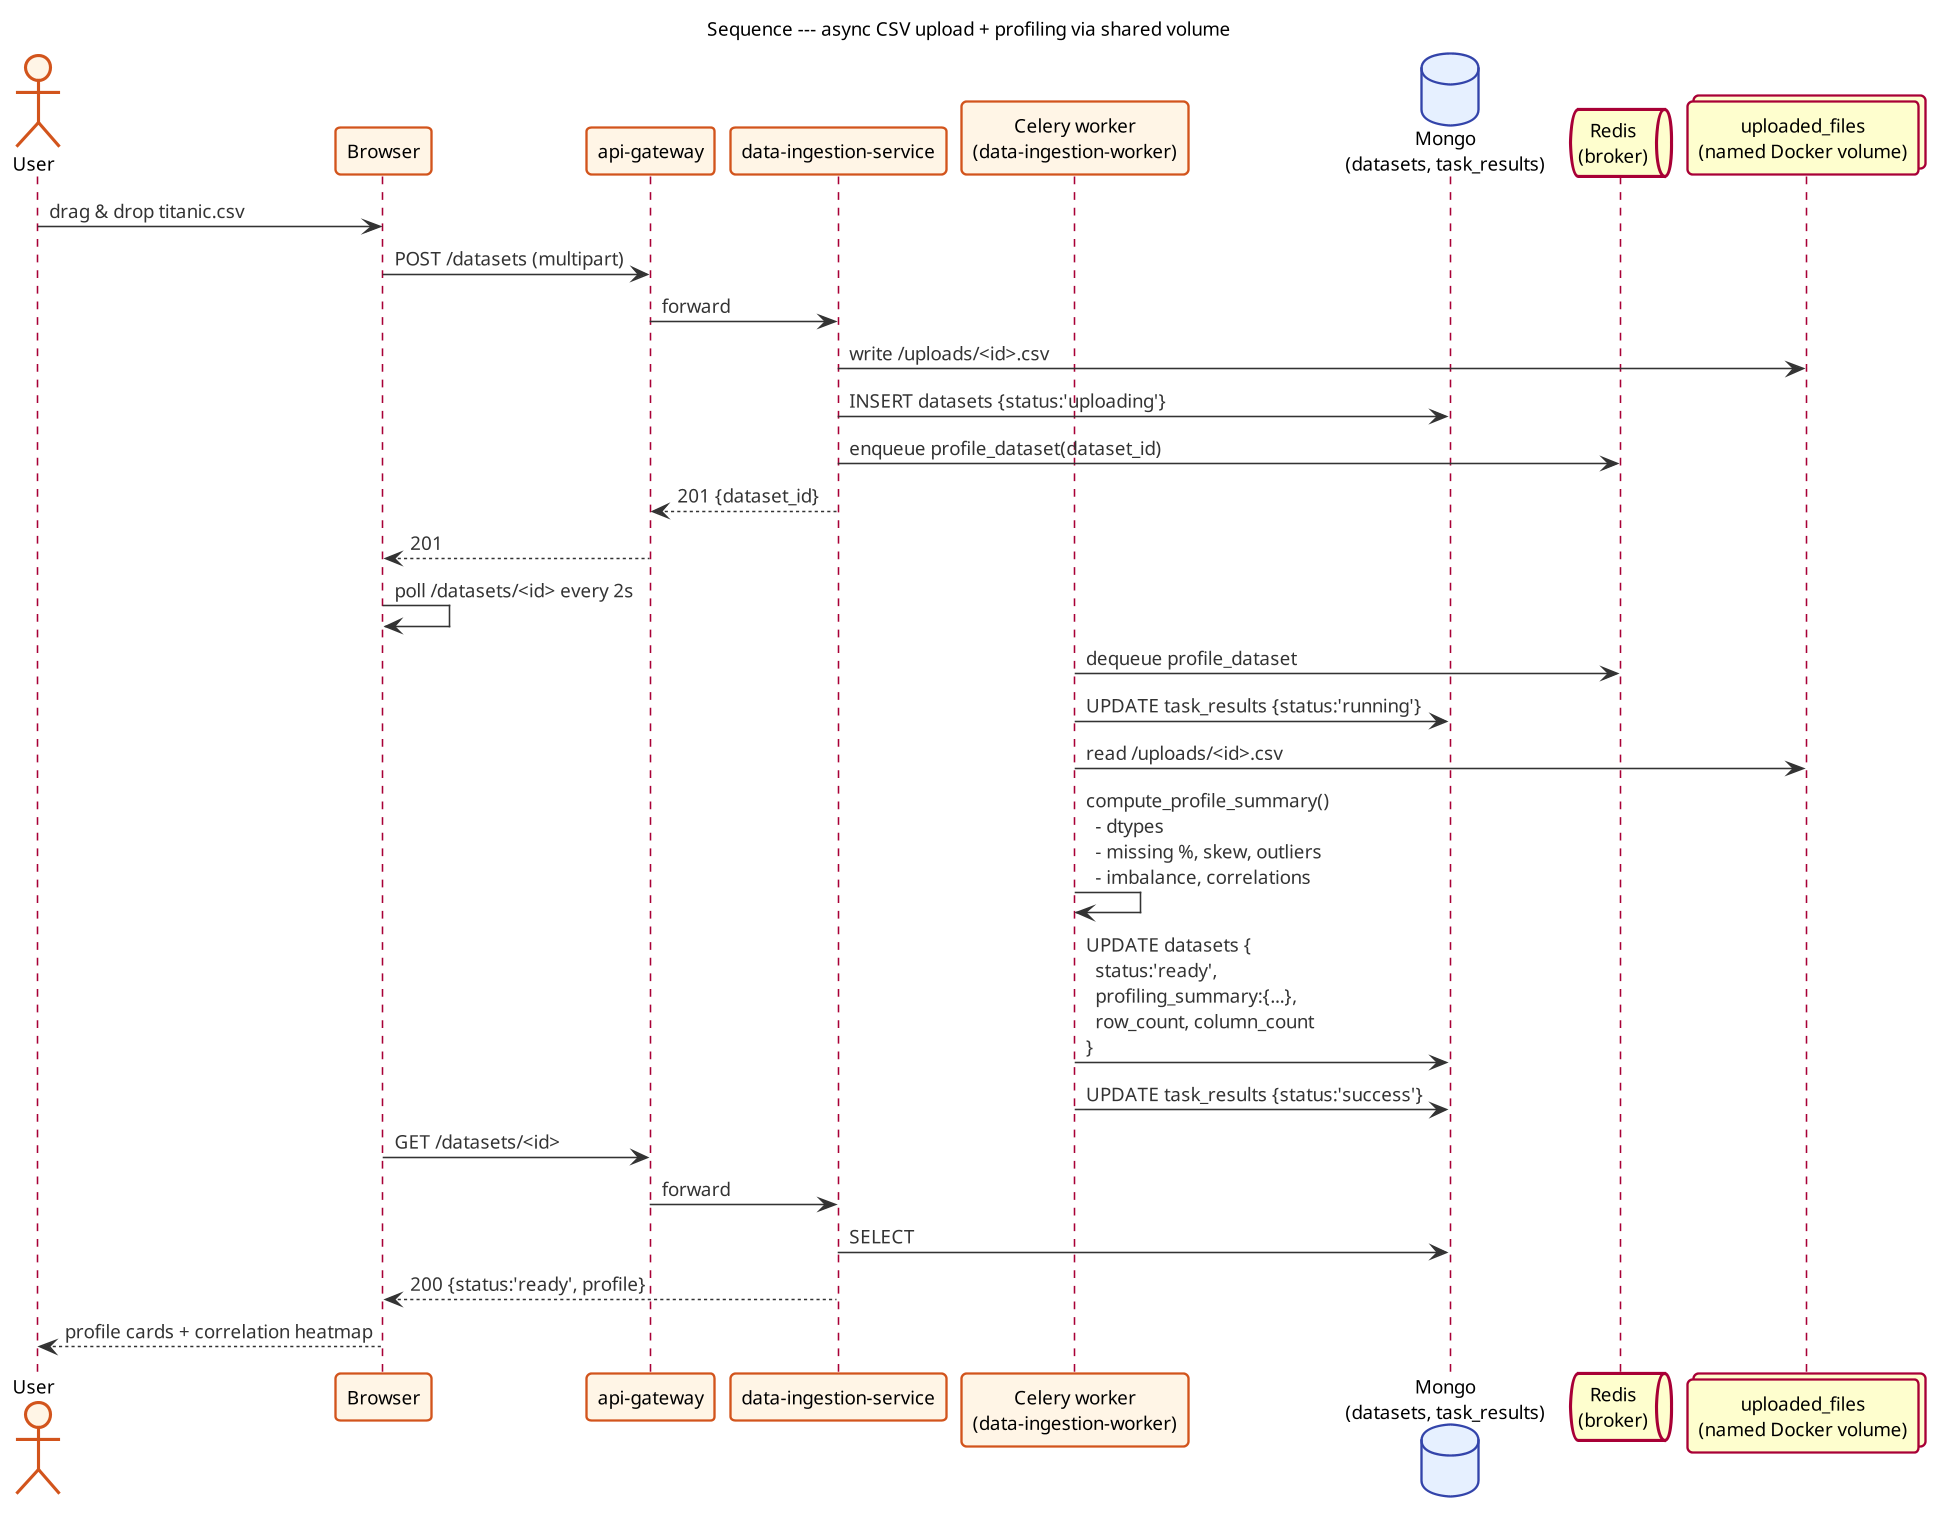
\includegraphics[width=0.85\textwidth, keepaspectratio]{diagrams/ch4_fig3}
  \caption{Sequence diagram --- upload plus asynchronous profiling.}
  \label{fig:ch4_fig3}
\end{figure}

\begin{figure}[H]
  \centering
  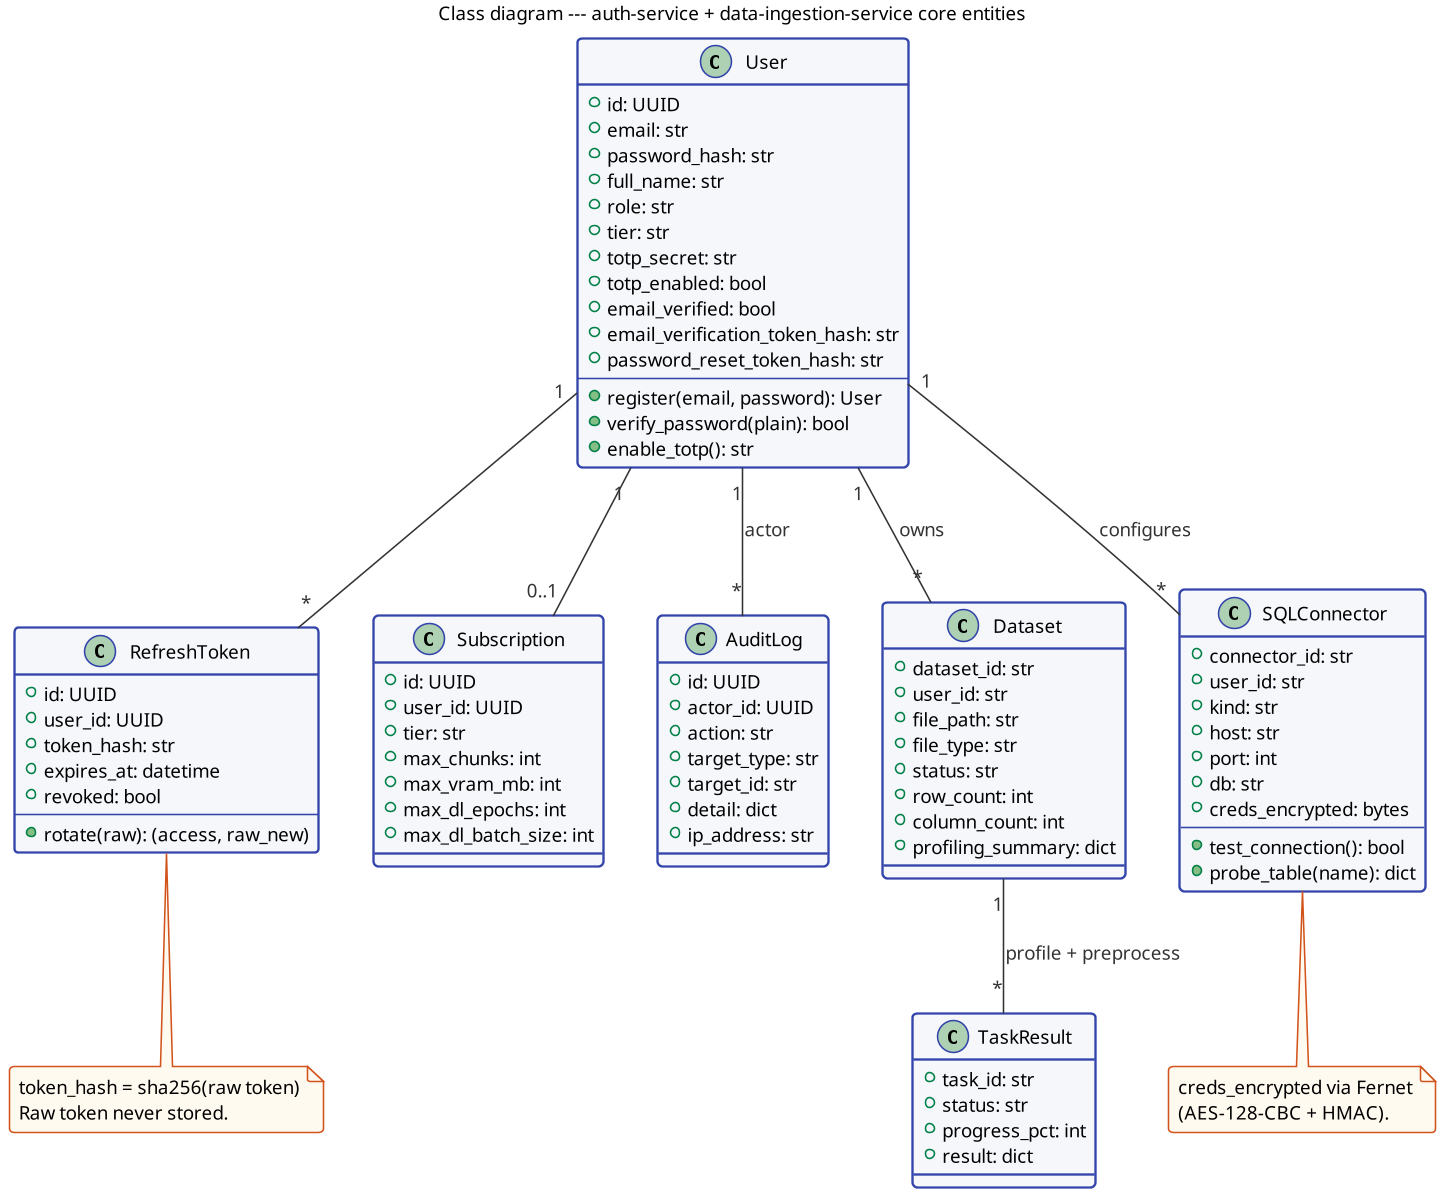
\includegraphics[width=0.85\textwidth, keepaspectratio]{diagrams/ch4_fig4}
  \caption{Class diagram --- auth-service plus data-ingestion-service.}
  \label{fig:ch4_fig4}
\end{figure}

\subsection{Why an opaque-but-decoded gateway}

Two reasonable architectures sat on the table.

\begin{enumerate}
    \item Have the gateway hit \texttt{auth-service} on every
        request to validate the JWT.
    \item Have the gateway hold the same \texttt{JWT\_SECRET\_KEY}
        as \texttt{auth-service} and decode the token in-process.
\end{enumerate}

The second option won, and we would make the same call again. The
gateway is on the hot path; a synchronous HTTP round-trip per
request adds latency that compounds badly under load. The price is
that the gateway needs the same signing secret as the auth service
--- which, in a shared environment-file deployment, is a non-issue.
A horizontally scaled production setup would need a key-distribution
mechanism; for the demo target the in-process decode is the right
trade.

\subsection{Header-injection rules}

The gateway strips any client-supplied \texttt{X-User-*},
\texttt{X-Company-*}, or \texttt{X-Project-*} header before
forwarding the request, then re-adds those headers from the
decoded JWT. This is the most important single security invariant
in the system. Downstream services trust \texttt{X-User-Id}
unconditionally, which means an attacker who can supply that header
without traversing the gateway can impersonate anyone. The
strip-then-inject pattern is deliberate, well tested, and not
negotiable.

\subsection{The shared-volume convention}

The first instinct on the ingestion side was to have the API stream
files to the worker over the network. That approach was built halfway
before a simpler one became obvious: the Docker Compose stack already
had a named volume (\texttt{uploaded\_files}) that both the API
container and the worker container could mount. Mounting it in both
places collapsed the streaming-upload protocol into a one-line write
--- the API saves to \texttt{/uploads/<id>.csv}, the worker reads
from the same path. That pattern then became the convention for
every binary artefact in the system: trained models, RAG documents,
and image-dataset extracts all live on named volumes mounted into
whichever services need them.

\subsection{Why MongoDB for dataset metadata}

A dataset's profile is fundamentally schemaless. A CSV with two
numeric columns produces a profile that looks nothing like the
profile of a CSV with thirty mixed-type columns and a target.
Postgres JSONB was considered for this storage and rejected. Mongo's
document model is lossless, queryable enough for the use case, and
imposes no schema migration when a new statistic is added in a later
sprint.

\section{Implementation}

\begin{lstlisting}[language=Python, caption=Gateway proxy with header injection (\texttt{api-gateway/app/routes/proxy.py})]
def _forward(upstream_base, path, require_auth=True, timeout=30):
    if require_auth:
        try:
            verify_jwt_in_request()
            claims = get_jwt()
            g.user_id = get_jwt_identity()
            g.user_role = claims.get("role", "")
            g.user_tier = claims.get("tier", "free")
        except Exception as e:
            return jsonify({"error": "unauthorized", "message": str(e)}), 401

    # Strip every client-supplied identity header before forwarding.
    _STRIP_PREFIXES = ("x-user-", "x-company-", "x-project-")
    headers = {
        k: v for k, v in request.headers
        if k.lower() not in _HOP_BY_HOP
        and k.lower() != "host"
        and not k.lower().startswith(_STRIP_PREFIXES)
    }
    # Re-inject the authoritative ones from the decoded JWT.
    if require_auth or hasattr(g, "user_id"):
        headers.update(get_forwarded_headers())

    resp = requests.request(
        method=request.method, url=f"{upstream_base.rstrip('/')}{path}",
        headers=headers, data=request.get_data(), stream=True, timeout=timeout,
    )
    return _stream_response(resp)
\end{lstlisting}

\begin{lstlisting}[language=Python, caption=Profiling task (\texttt{data-ingestion-service/app/tasks/profiling.py})]
@celery.task(name="app.tasks.profiling.profile_dataset", bind=True)
def profile_dataset(self, dataset_id: str):
    client = MongoClient(os.environ["MONGO_URL"])
    db = client[os.environ.get("MONGO_DB", "nocode_ingestion")]
    datasets = db["datasets"]
    task_results = db["task_results"]

    task_results.update_one(
        {"task_id": self.request.id},
        {"$set": {"status": "running", "progress_pct": 0}},
        upsert=True,
    )
    doc = datasets.find_one({"dataset_id": dataset_id})
    df = load_dataframe(doc["file_path"])

    summary = compute_profile_summary(df, target_column=doc.get("target_column"))

    datasets.update_one(
        {"dataset_id": dataset_id},
        {"$set": {
            "status": "ready",
            "profiling_summary": summary,
            "row_count": len(df),
            "column_count": len(df.columns),
        }},
    )
    task_results.update_one(
        {"task_id": self.request.id},
        {"$set": {"status": "success", "progress_pct": 100}},
    )
\end{lstlisting}

\subsection{Security posture}

\begin{itemize}
    \item Access tokens carry a fifteen-minute TTL. Refresh tokens
        live as HttpOnly cookies and rotate on every refresh; the
        previous token's JTI lands in the Redis blacklist so a
        stolen refresh token can actually be revoked.
    \item Passwords use \texttt{bcrypt} at cost~12. Refresh tokens
        themselves are stored as SHA-256 hashes in Postgres --- the
        database-breach scenario yields a hash, not a usable token.
    \item TOTP-based two-factor authentication is optional per user;
        super-admins can require it per-tier from the admin panel.
    \item Per-IP and per-user rate limits sit at the gateway. The
        per-user limit defaults to $600$\,req/min in development,
        deliberately loose because React~18 Strict Mode
        double-invokes \texttt{useEffect} and a tighter cap was
        producing spurious 429s. Production caps tighten to
        $120$\,req/min.
\end{itemize}

\subsection{SQL connectors and Fernet encryption}

Users can configure a Postgres or MySQL connector inside the
platform. Credentials are encrypted with a Fernet key
(AES-128-CBC plus HMAC) held in the service's environment, then
stored in Mongo. The same key is reused for any other secret the
ingestion service needs to hold, and rotation is a documented
operations procedure rather than a fire-fight. SQL queries themselves
run through SQLAlchemy with parameter binding, which makes SQL
injection structurally impossible rather than merely unlikely.

\begin{figure}[H]
  \centering
  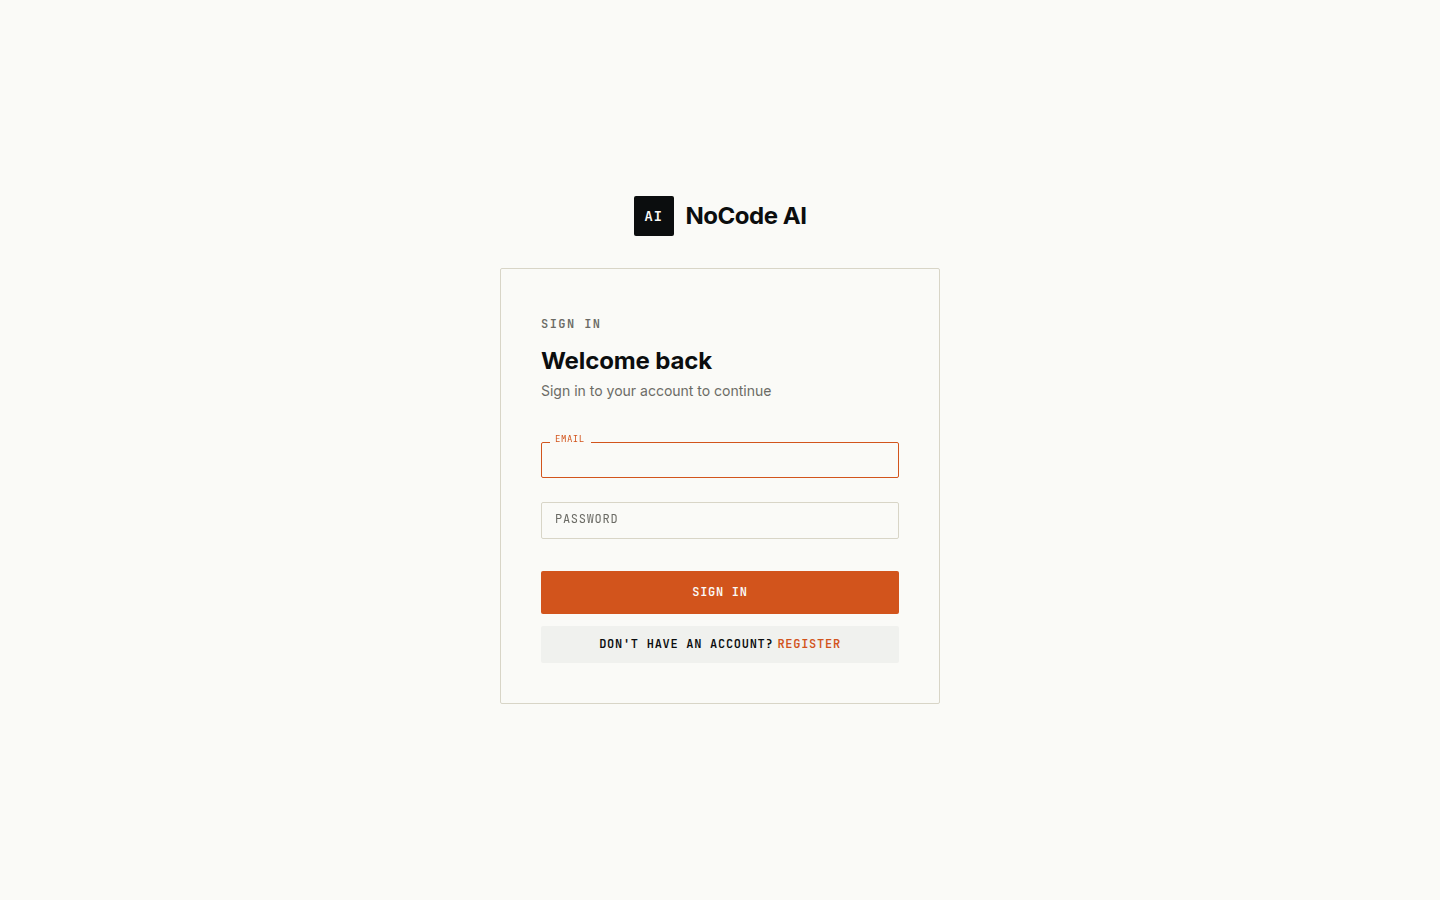
\includegraphics[width=0.85\textwidth, keepaspectratio]{diagrams/ch4_fig5}
  \caption{Login screen with optional TOTP field.}
  \label{fig:ch4_fig5}
\end{figure}

\begin{figure}[H]
  \centering
  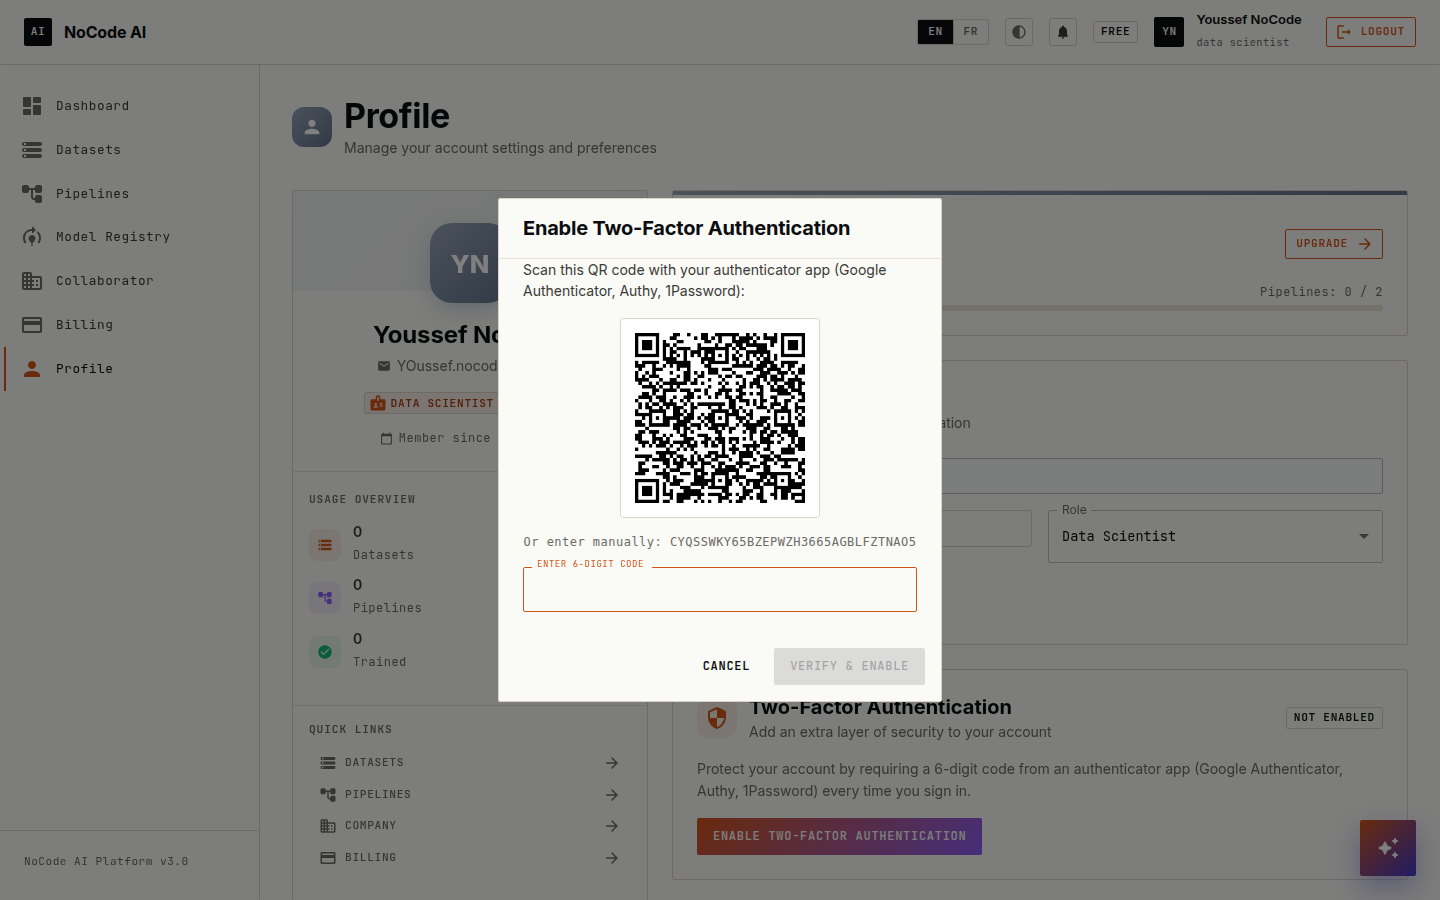
\includegraphics[width=0.85\textwidth, keepaspectratio]{diagrams/ch4_fig6}
  \caption{SQL connector wizard --- credentials encrypted at rest.}
  \label{fig:ch4_fig6}
\end{figure}

\begin{figure}[H]
  \centering
  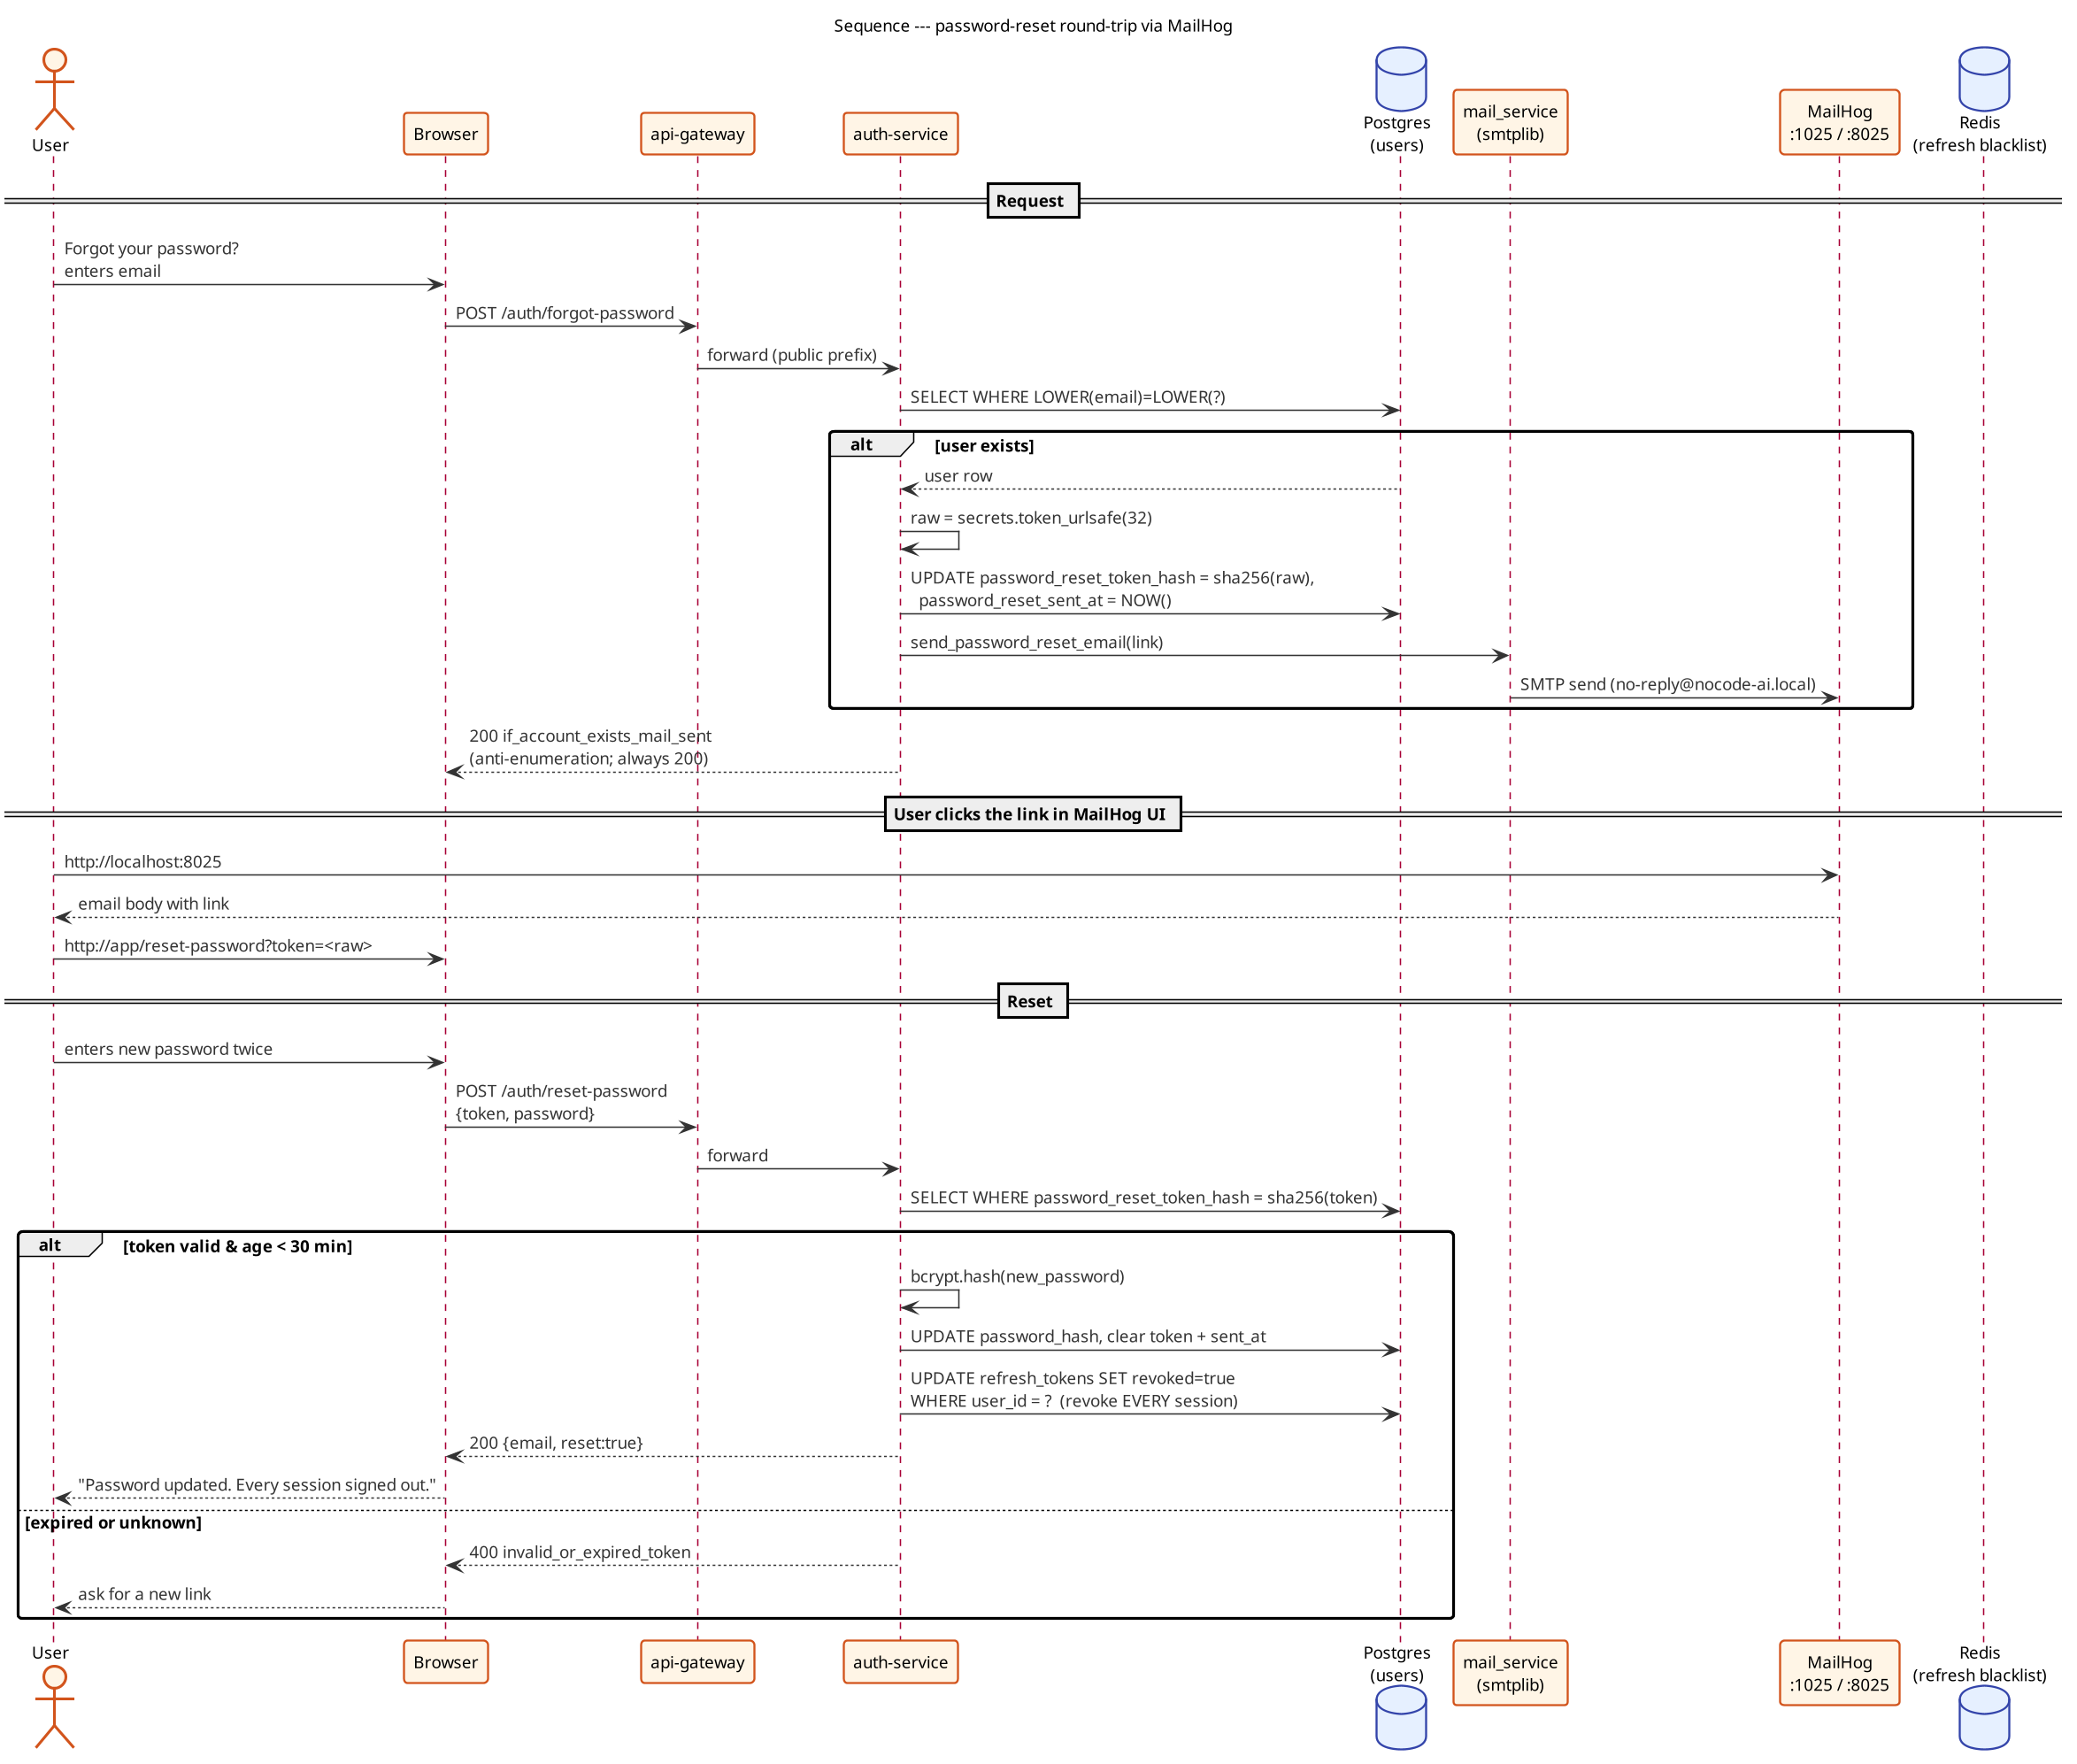
\includegraphics[width=0.85\textwidth, keepaspectratio]{diagrams/ch4_fig_seq_password_reset}
  \caption{Sequence diagram --- password-reset round-trip via MailHog.}
  \label{fig:ch4_fig_seq_password_reset}
\end{figure}

\section{Unit Tests}

The auth-service test suite covers more than $80\%$ of the
authentication path and the admin operations. Notable cases:

\begin{itemize}
    \item Forged \texttt{X-User-Id} header: the request passes
        through the gateway, the forged header is stripped, the
        authoritative one from the JWT replaces it. Asserted on a
        synthetic upstream that echoes back the headers it saw.
    \item Refresh-token replay: a refresh token is used once, then
        replayed. The second use is rejected by the blacklist.
    \item Expired access token: the gateway returns 401 with the
        documented error envelope.
    \item Rate limit: 601 requests in one minute, the 601st returns
        429 with a \texttt{Retry-After} header.
\end{itemize}

The ingestion suite uses \texttt{mongomock} so it does not need a
real Mongo to run. It exercises the upload-then-profile path
end-to-end with a small fixture CSV and asserts the profile shape.

\section*{Conclusion}

By the end of Sprint~1 the platform had end-to-end authentication, a
working refresh-token loop, a gateway pattern the next five sprints
would build on, and an ingestion service that profiled arbitrarily
messy CSVs asynchronously. The authoritative-headers convention
became one of the project's most quietly useful design decisions ---
every subsequent service trusts \texttt{X-User-Id} without a second
thought, because the gateway is the only path along which it can be
set.

% ═════════════════════════════════════════════════════════════════════════════
\chapter{Sprint 2: Visual Pipeline Editor and Tabular Machine Learning}
% ═════════════════════════════════════════════════════════════════════════════

\section*{Introduction}

Sprint~2 was the largest single sprint of the project. It pulled
together four pieces --- the visual pipeline editor, the
\texttt{ml-training-service} with its fourteen tabular algorithms,
the live metric visualisations, and the post-training surface (SHAP
explainability, model export) --- into a coherent flow that a user
could follow from canvas to artefact.

\section{Sprint Backlog}

\begin{table}[H]
\centering
\caption{Sprint~2 backlog --- canvas plus tabular ML stack.}
\label{tab:sprint2_backlog}
\begin{tabular}{@{}p{0.05\linewidth} L{0.55\linewidth} p{0.1\linewidth} p{0.18\linewidth}@{}}
\toprule
\textbf{ID} & \textbf{User Story / Task} & \textbf{Priority} & \textbf{Estimation (d)} \\
\midrule
US-12 & React Flow canvas with custom node components and per-node validation. & High & 3 \\
US-13 & Pipeline schema (Mongo document with nodes + edges). & High & 0.5 \\
US-14 & \texttt{ml-training-service} hosting fourteen tabular algorithms. & High & 4 \\
US-15 & \texttt{BaseMLModel} abstraction + algorithm-agnostic Celery task. & High & 1 \\
US-16 & Model registry with versioning. & High & 1 \\
US-17 & Live metric streaming over SocketIO. & Medium & 1.5 \\
US-18 & SHAP explainability for supervised runs (TreeExplainer fast path). & Medium & 1 \\
US-19 & Confusion matrices and residual plots. & Medium & 0.5 \\
US-20 & Model export (joblib + generated FastAPI inference script). & Medium & 1 \\
\bottomrule
\end{tabular}
\end{table}

\section{CRISP-DM applied to the tabular ML sprint}

We framed the ML work through the CRISP-DM lifecycle. The mapping
makes it concrete what each phase delivered for this project.

\begin{figure}[H]
  \centering
  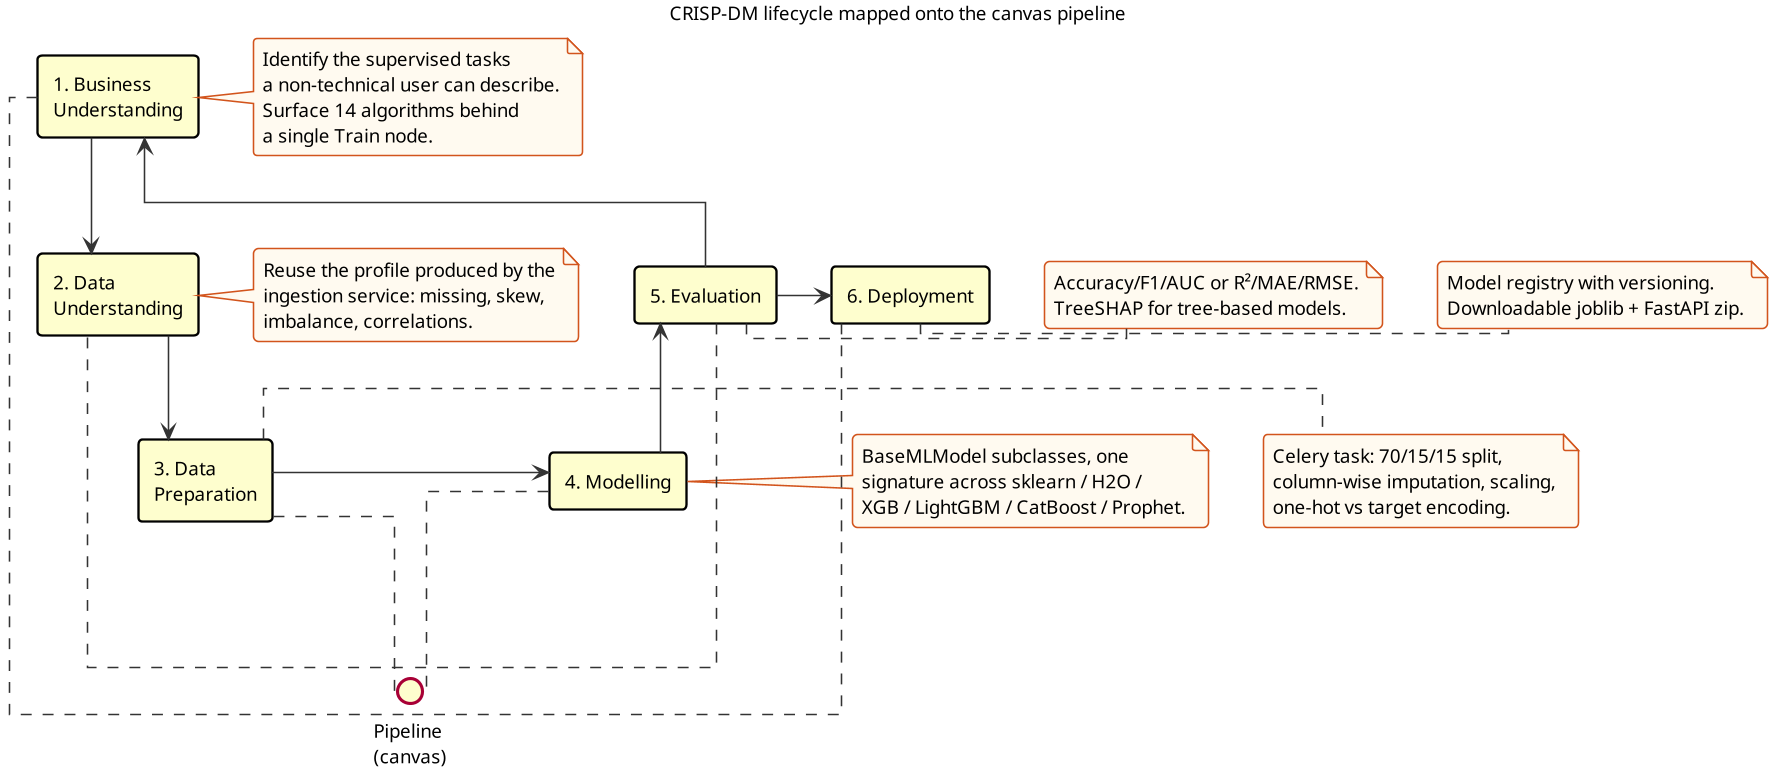
\includegraphics[width=0.85\textwidth, keepaspectratio]{diagrams/ch5_fig_crispdm}
  \caption{CRISP-DM lifecycle mapped onto the Sprint~2 pipeline.}
  \label{fig:ch5_fig_crispdm}
\end{figure}

\begin{table}[H]
\centering
\caption{CRISP-DM phases mapped to Sprint~2 deliverables.}
\label{tab:crispdm}
\begin{tabular}{@{}p{0.22\linewidth} L{0.7\linewidth}@{}}
\toprule
\textbf{CRISP-DM phase} & \textbf{What this sprint delivered} \\
\midrule
Business understanding & Identify the supervised tasks a non-technical user can describe (classification, regression, clustering, forecasting). Surface fourteen named algorithms behind one shared canvas node. \\
Data understanding & Reuse the ingestion-service profile: missing values, skew, target imbalance, correlation. Surface alerts on the canvas's Dataset node. \\
Data preparation & Celery preprocessing task: 70/15/15 train/val/test split, column-wise imputation, scaling for distance-based algorithms, one-hot or target encoding by cardinality. \\
Modelling & \texttt{BaseMLModel} subclasses construct, fit, predict, and evaluate against a shared signature regardless of underlying library (sklearn, XGBoost, LightGBM, CatBoost, H2O, Prophet). \\
Evaluation & Accuracy/F1/AUC for classification, R$^2$/MAE/RMSE for regression. F1 is preferred in the summary card when the target is imbalanced. SHAP feature importance for tree-based supervised runs. \\
Deployment & Versioned artefact in the registry; downloadable joblib + FastAPI launcher zip. Re-running a pipeline mints a new version rather than overwriting. \\
\bottomrule
\end{tabular}
\end{table}

\section{Design}

\begin{figure}[H]
  \centering
  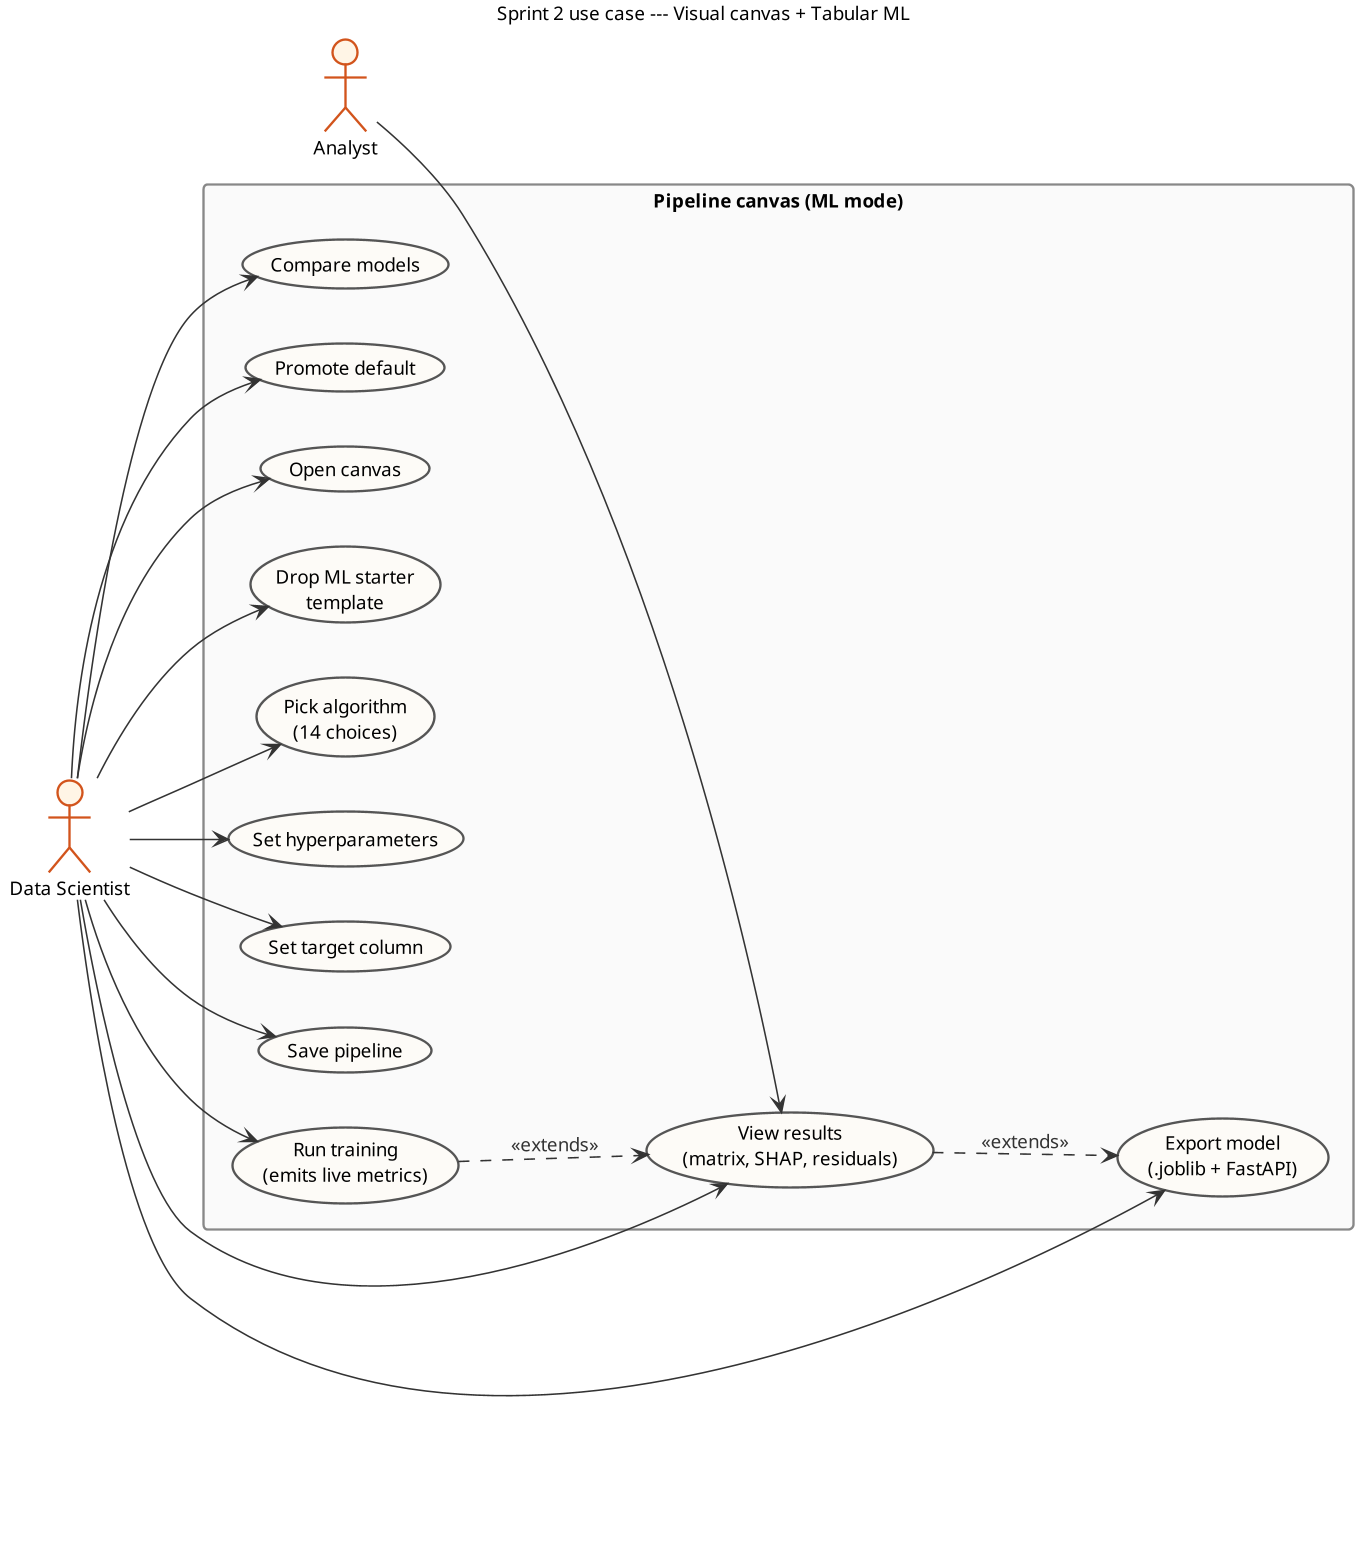
\includegraphics[width=0.85\textwidth, keepaspectratio]{diagrams/ch5_fig1}
  \caption{Use case diagram --- canvas plus tabular ML.}
  \label{fig:ch5_fig1}
\end{figure}

\begin{landscape}
\begin{figure}[H]
  \centering
  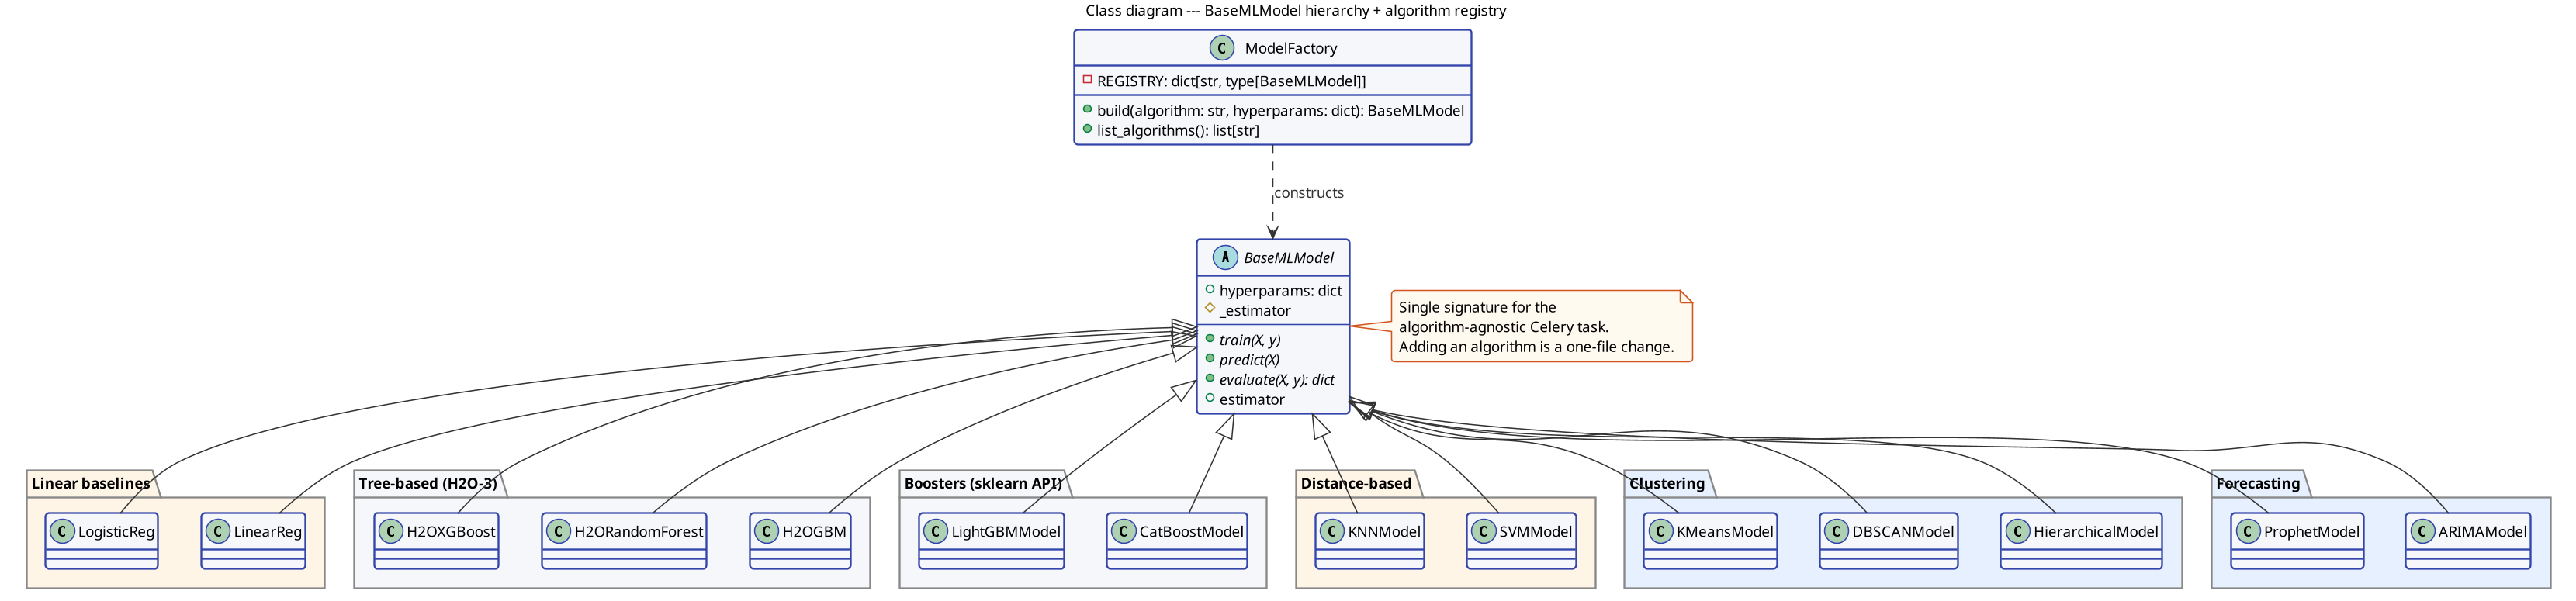
\includegraphics[width=0.95\linewidth, keepaspectratio]{diagrams/ch5_fig2}
  \caption{Class diagram --- BaseMLModel hierarchy and the algorithm registry.}
  \label{fig:ch5_fig2}
\end{figure}
\end{landscape}

% [FIGURE NEEDED: Pipeline editor screenshot in ML mode --- Dataset, Train, Evaluate nodes with the live metric chart below]
% \begin{figure}[H]
%   \centering
%   \includegraphics[width=0.95\textwidth]{figures/placeholder_ch5_fig3}
%   \caption{Pipeline editor in tabular ML mode.}
%   \label{fig:ch5_fig3}
% \end{figure}

\begin{landscape}
\begin{figure}[H]
  \centering
  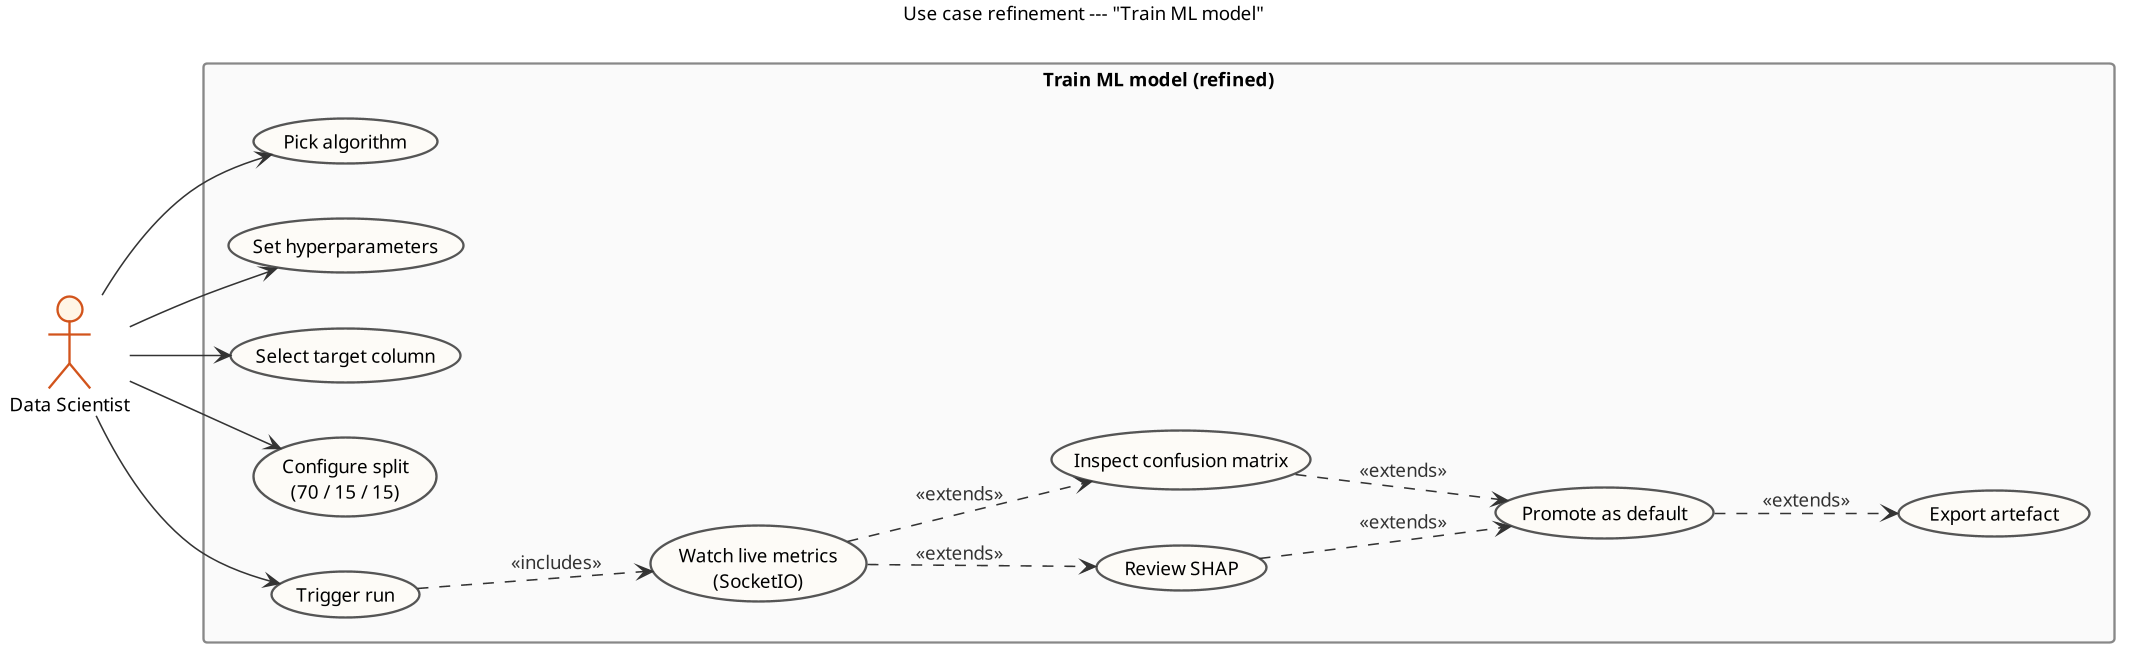
\includegraphics[width=0.95\linewidth, keepaspectratio]{diagrams/ch5_fig_uc_refine_train}
  \caption{Use-case refinement --- ``Train ML model'' broken into sub-cases.}
  \label{fig:ch5_fig_uc_refine_train}
\end{figure}
\end{landscape}

\begin{figure}[H]
  \centering
  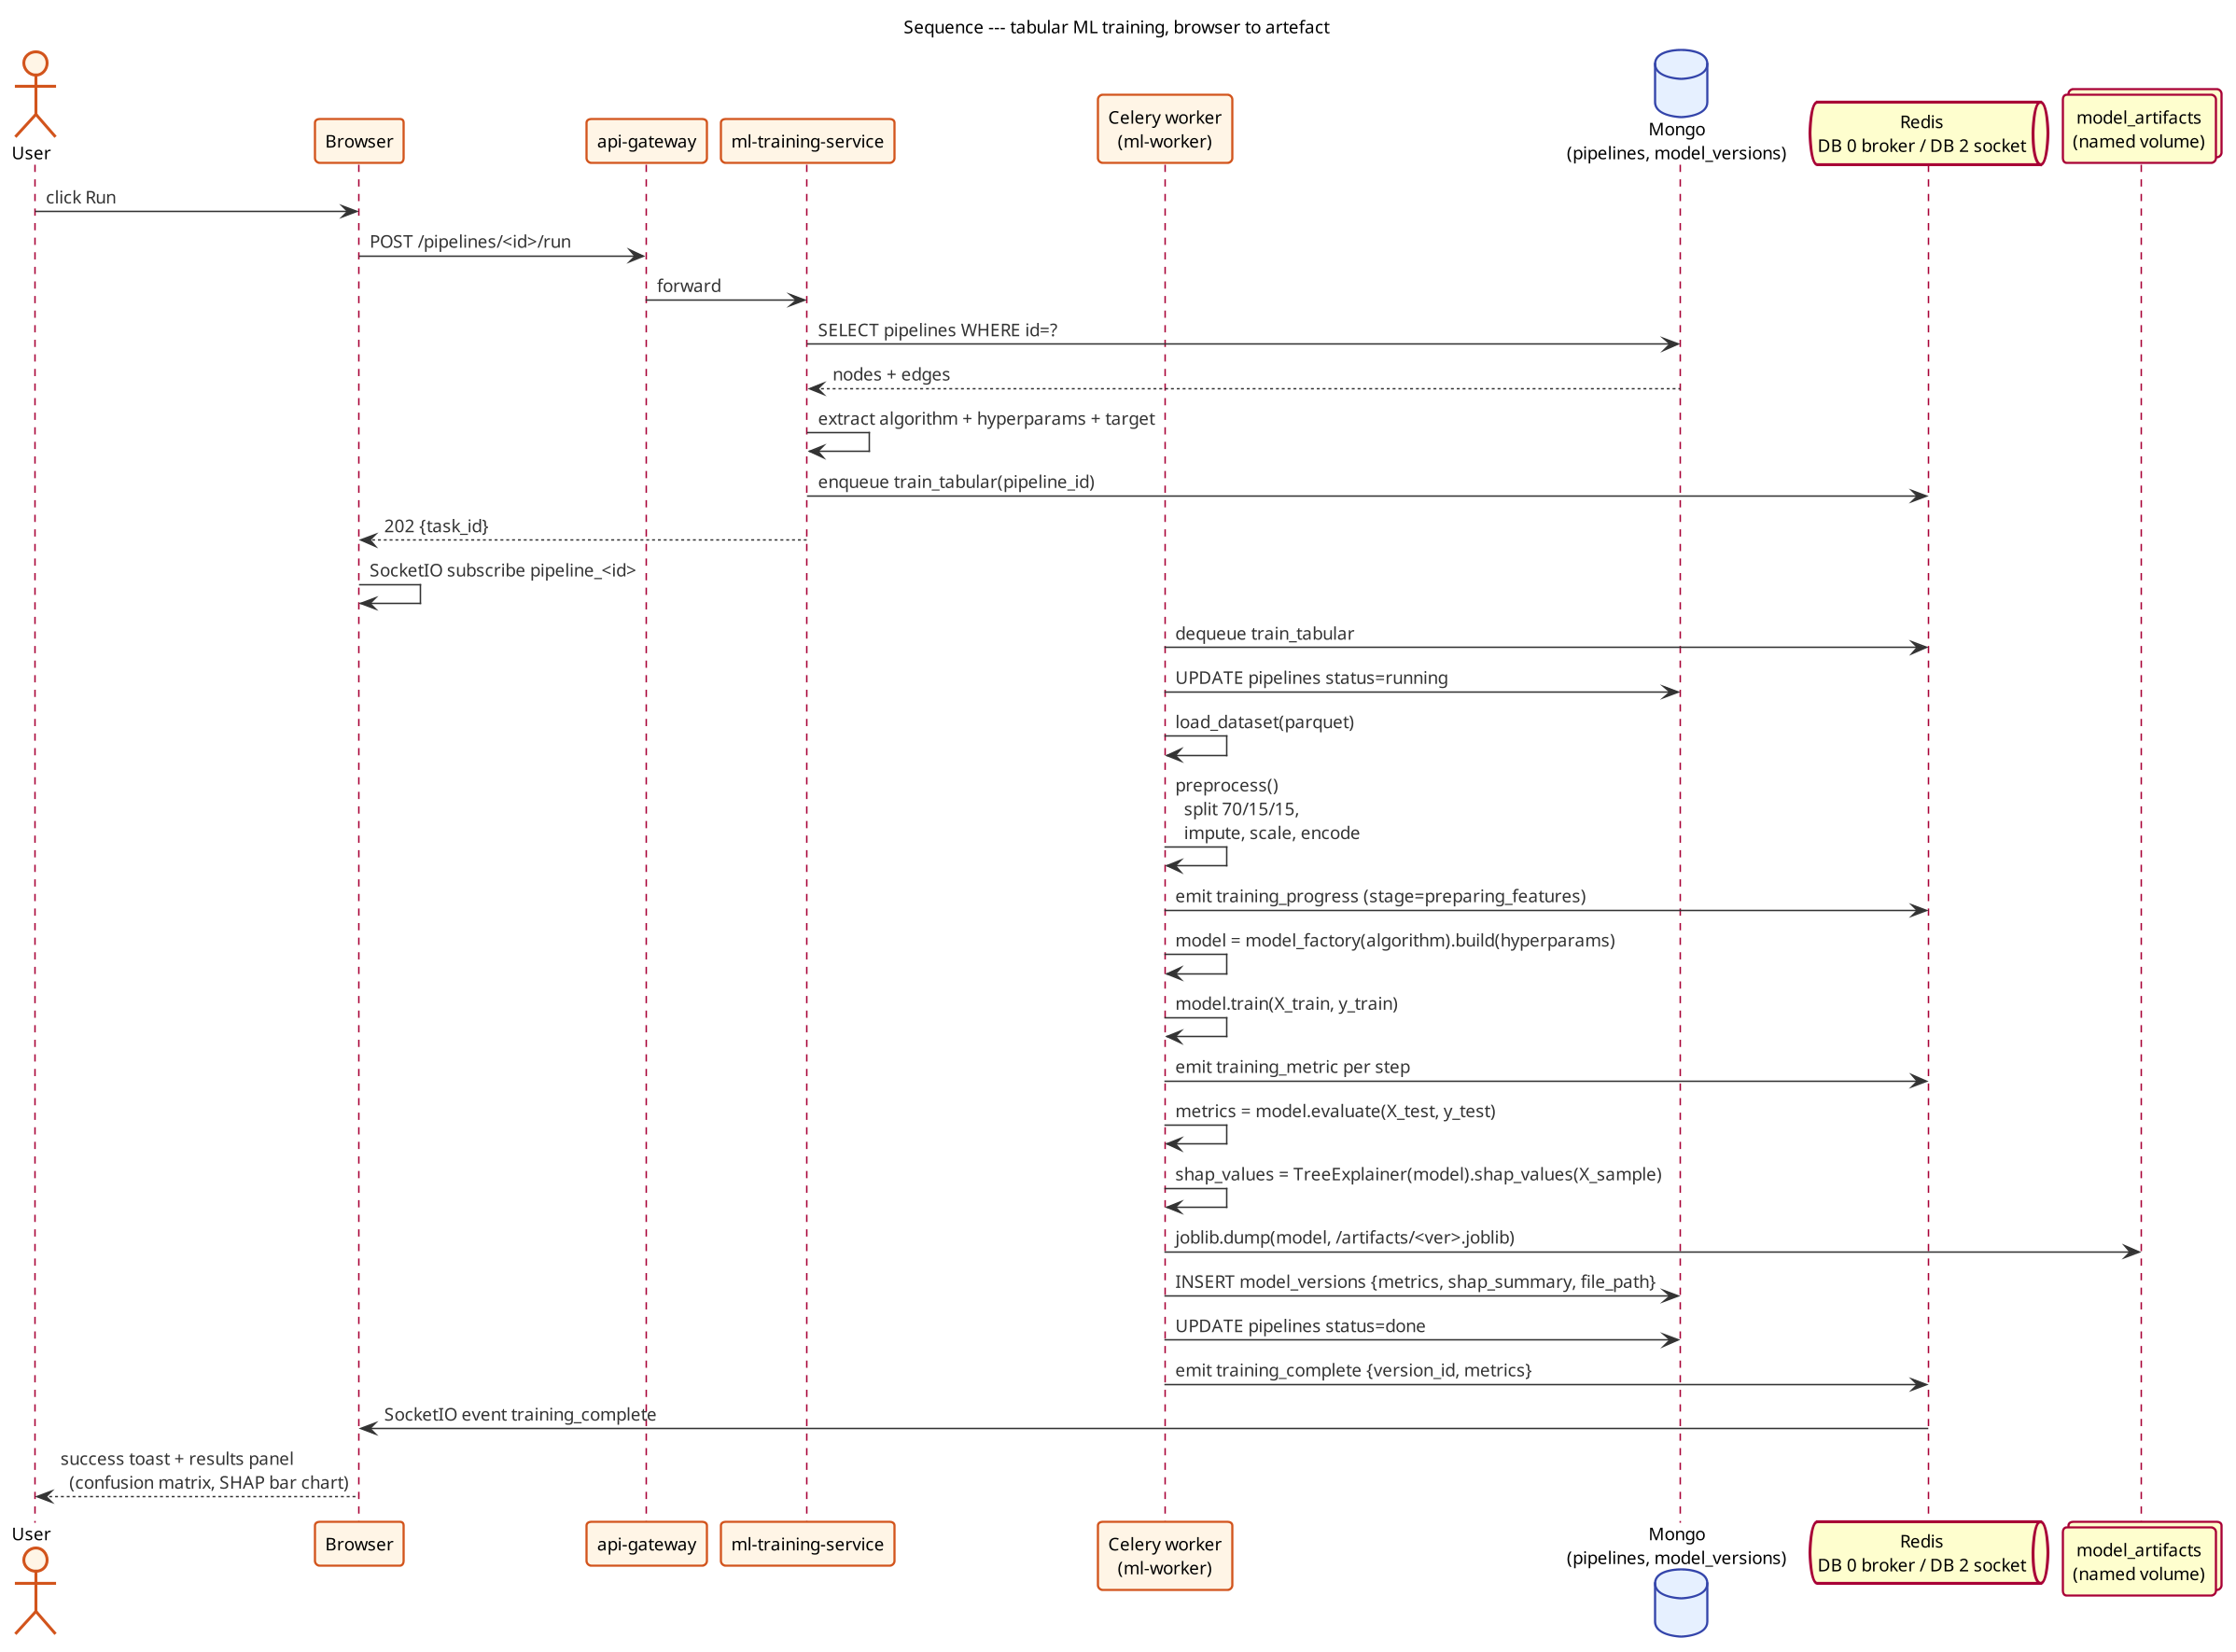
\includegraphics[width=0.85\textwidth, keepaspectratio]{diagrams/ch5_fig_seq_training}
  \caption{Sequence diagram --- tabular ML training, browser to artefact.}
  \label{fig:ch5_fig_seq_training}
\end{figure}

\begin{figure}[H]
  \centering
  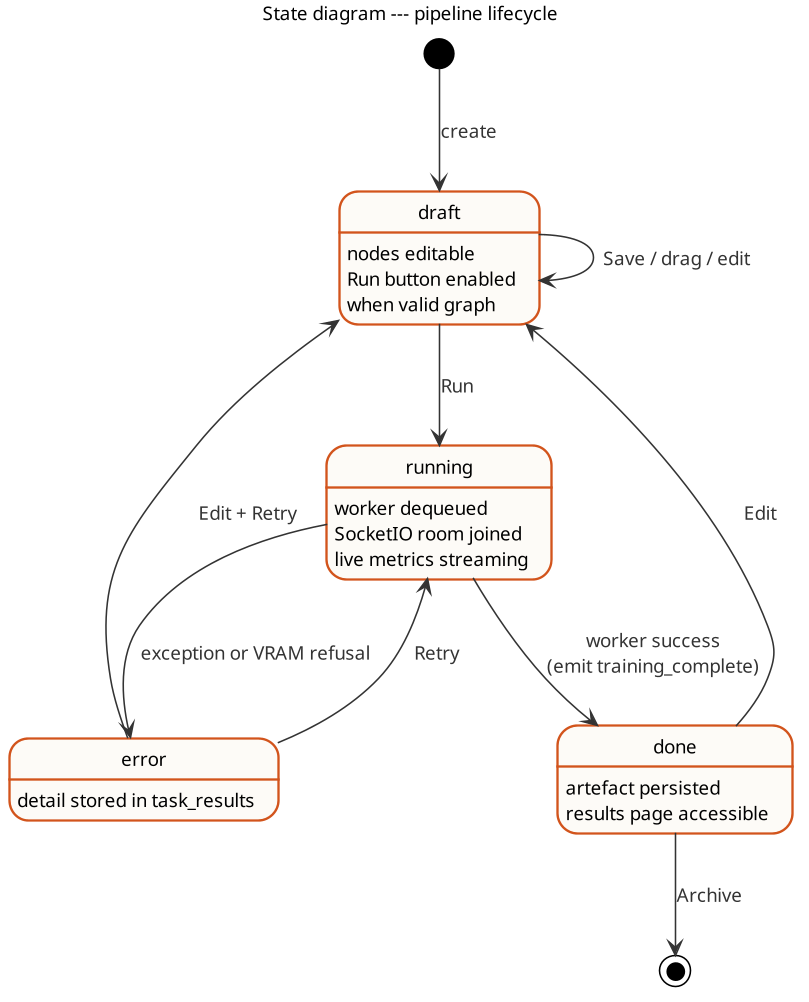
\includegraphics[width=0.85\textwidth, keepaspectratio]{diagrams/ch5_fig_state_pipeline}
  \caption{State diagram --- pipeline lifecycle transitions.}
  \label{fig:ch5_fig_state_pipeline}
\end{figure}

\subsection{Graph schema}

A pipeline is stored in Mongo as a document with two arrays:

\begin{lstlisting}[language=JSON, caption=Pipeline document shape]
{
  "pipeline_id": "...",
  "user_id": "...",
  "type": "ml" | "rag" | "dl",
  "nodes": [
    { "node_id": "n1", "type": "dataset", "position": {"x": 60, "y": 120},
      "data": { "dataset_id": "..." } },
    { "node_id": "n2", "type": "train", "position": {"x": 320, "y": 120},
      "data": { "algorithm": "xgboost", "task_type": "classification",
                "hyperparams": {...}, "target_column": "..." } },
    { "node_id": "n3", "type": "evaluate", "position": {"x": 580, "y": 120},
      "data": {} }
  ],
  "edges": [
    { "source": "n1", "target": "n2" },
    { "source": "n2", "target": "n3" }
  ],
  "status": "draft"|"running"|"done"|"error"
}
\end{lstlisting}

\subsection{The \texttt{BaseMLModel} abstraction}

Fourteen algorithms with one orchestrator implies an abstraction.
Rather than over-engineer it, we used a deliberately small abstract
base class. Each algorithm subclass exposes \texttt{train},
\texttt{predict}, and \texttt{evaluate} with a shared signature,
whether it wraps scikit-learn, XGBoost, LightGBM, CatBoost, or
Prophet. The training Celery task is algorithm-agnostic: it
constructs a model from a registry, trains it, asks for metrics, and
serialises the estimator. Adding a new algorithm is, in practice, a
one-file change.

\begin{lstlisting}[language=Python, caption=Algorithm-agnostic training core]
class BaseMLModel(ABC):
    def __init__(self, hyperparams: dict[str, Any]):
        self.hyperparams = hyperparams
        self._estimator = None

    @abstractmethod
    def train(self, X_train, y_train=None) -> None: ...
    @abstractmethod
    def predict(self, X) -> Any: ...
    @abstractmethod
    def evaluate(self, X_test, y_test=None) -> dict[str, Any]: ...

    @property
    def estimator(self):
        return self._estimator
\end{lstlisting}

The registry mapping algorithm strings to subclasses lives in
\texttt{ml-training-service/app/services/model\_factory.py}.

\subsection{Algorithm selection}

The fourteen algorithms span four task families. The choice in each
family was driven by the trade-off between training time, accuracy on
typical tabular shapes, and how cleanly each library integrates with
the abstraction above.

\textbf{Classification and regression.} For tree-based methods,
XGBoost is the default because boosted trees consistently dominate on
structured data with mixed numerical and categorical features ---
they capture non-linear feature interactions without explicit
feature engineering, and the H2O implementation we use ships
TreeSHAP for fast post-hoc explanation. Random Forest and Gradient
Boosting Machines are exposed as alternatives for users who prefer
simpler hyperparameter surfaces. Linear and logistic regression sit
alongside the boosters as fast, interpretable baselines for small or
very wide datasets where a tree's overhead is not justified.

\textbf{Clustering.} K-Means is the default for its O(nkd) cost and
predictable behaviour; DBSCAN is exposed for data with non-spherical
clusters; hierarchical agglomeration sits as a third option for
small datasets where a dendrogram is more useful than a label.

\textbf{Forecasting.} Prophet is the default for time series with
seasonal or holiday components, and it is one of the few algorithms
where the cost of a compile-from-source dependency (CmdStan) is
genuinely worth paying. ARIMA is the alternative for series that are
already stationary or short.

\textbf{Heavy lifting on H2O.} For XGBoost, GBM, and Random Forest,
the platform uses H2O-3 in place of the scikit-learn implementations.
H2O's algorithms run faster on tabular data, parallelise across the
host's CPU cores by default, and expose feature importance plus SHAP
values out of the box --- which removed an entire subtask from the
explainability work.

\begin{table}[H]
\centering
\caption{Algorithm catalogue for the tabular ML mode.}
\label{tab:ml_algos}
\begin{tabular}{@{}L{0.21\linewidth} L{0.16\linewidth} L{0.16\linewidth} L{0.4\linewidth}@{}}
\toprule
\textbf{Algorithm} & \textbf{Task} & \textbf{Backend} & \textbf{Why it is in the catalogue} \\
\midrule
Logistic Regression & Classification & scikit-learn & Fast linear baseline, interpretable coefficients. \\
Linear Regression & Regression & scikit-learn & Baseline for continuous targets, residual diagnostics. \\
Random Forest & Both & H2O-3 & Robust default, no scaling needed, OOB error estimate. \\
XGBoost & Both & H2O-3 & Highest accuracy on most tabular data with interactions. \\
LightGBM & Both & scikit-learn API & Faster than XGBoost on wide datasets, leaf-wise growth. \\
CatBoost & Both & scikit-learn API & Native categorical handling without one-hot blow-up. \\
GBM & Both & H2O-3 & Mature gradient boosting, stable on small data. \\
K-Means & Clustering & scikit-learn & Default for spherical clusters, O(nkd) cost. \\
DBSCAN & Clustering & scikit-learn & Density-based, handles non-spherical clusters. \\
Hierarchical & Clustering & scikit-learn & Dendrogram visualisation on small datasets. \\
KNN & Both & scikit-learn & Non-parametric baseline, useful for sanity checks. \\
SVM & Classification & scikit-learn & Maximum-margin classifier for small clean datasets. \\
Prophet & Forecasting & Meta Prophet & Time series with seasonality and holiday effects. \\
ARIMA & Forecasting & statsmodels & Stationary or already-detrended series. \\
\bottomrule
\end{tabular}
\end{table}

\section{Implementation}

\subsection{Frontend canvas}

% [FIGURE NEEDED: Anatomy of a canvas node --- header with status, body with summary, input/output ports, validation badge in the corner]
% \begin{figure}[H]
%   \centering
%   \includegraphics[width=0.85\textwidth]{figures/placeholder_ch5_fig4}
%   \caption{Anatomy of a canvas node component.}
%   \label{fig:ch5_fig4}
% \end{figure}

The canvas is a React Flow instance with custom node components.
Each node type validates itself against the surrounding graph: the
\texttt{Train} node shows an error badge if no \texttt{Dataset} node
sits upstream, and the \texttt{Evaluate} node shows a warning if no
training run has produced a version yet. The validation function is
pure ---
\texttt{(node, edges, allNodes) $\to$ \{status, message\}} --- which
makes it trivially testable. Errors render inline rather than as
modal dialogs, so the user can fix three problems at once without
clicking through three pop-ups.

\subsection{Preprocessing and feature handling}

Before a model sees a single row, the preprocessing Celery task
splits the dataset into train / validation / test (default
$70$/$15$/$15$, configurable on the Train node), imputes missing
values column-wise, scales numerical features when the algorithm
requires it (logistic regression, K-Means), and encodes categorical
columns using one-hot for low-cardinality columns and target encoding
for high-cardinality ones. The transformer pipeline is stored
alongside the model artefact so inference applies the same
transformations to new rows.

\subsection{Live training visualisation}

Training emits per-step metric points over the SocketIO message
queue. The \texttt{LiveTrainingChart} component subscribes to the
pipeline's room (\texttt{pipeline\_<id>}) on the \texttt{/training}
namespace and plots the points on a Plotly scatter. The Y-axis is
auto-scaled because progress percentage ($0$--$100$) and metric
values (typically $0$--$1$) live on different ranges --- progress on
the primary axis, metrics on the secondary. A small detail, but the
chart was unreadable until that split landed.

\begin{figure}[H]
  \centering
  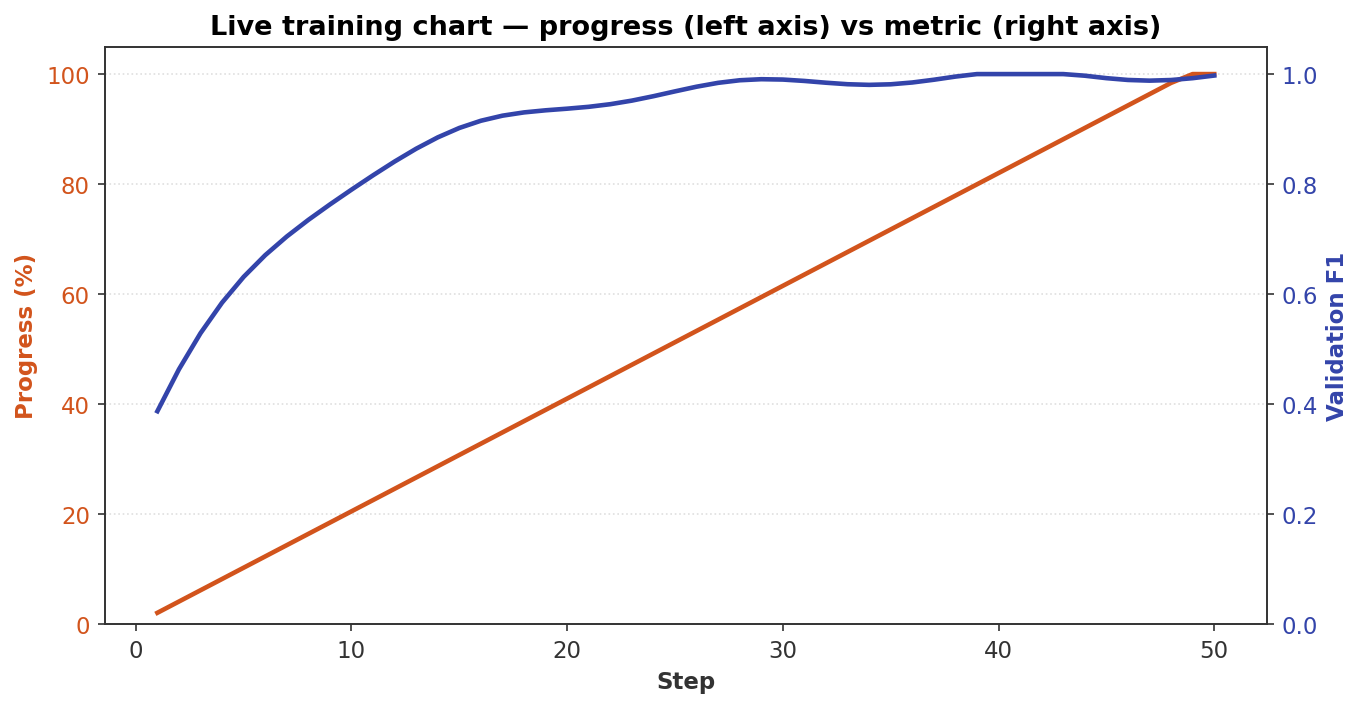
\includegraphics[width=0.85\textwidth, keepaspectratio]{diagrams/ch5_fig5}
  \caption{Live training chart --- progress on the primary axis, metric on the secondary.}
  \label{fig:ch5_fig5}
\end{figure}

\subsection{Evaluation and metric interpretation}

For classification runs, the platform reports accuracy, precision,
recall, F1, and ROC-AUC when the task is binary or one-versus-rest
multiclass. The validation report flags imbalanced targets (minority
class below $20\%$) and prefers F1 over raw accuracy in the
summary card, because accuracy on imbalanced data lies to the user.
For regression, the report ships R$^2$, mean absolute error, root
mean squared error, and the residual distribution as a histogram ---
R$^2$ alone is misleading on heavy-tailed errors, and the histogram
catches that visually.

The reference validation run uses a $250{,}000$-row salary dataset
with a Random Forest regressor and lands at an R$^2$ of $0.9785$ in
$4$\,min\,$12$\,s on the demo box. That score means roughly $97.85\%$
of the salary variance is explained by the features --- not a
production-grade number on a real dataset where the residuals would
need closer inspection, but a defensible result for a synthetic
benchmark that exercises the full canvas-to-artefact path.

\subsection{SHAP and the explainability surface}

Every supervised training run computes SHAP values over a sampled
subset of the test set. The bar chart of mean absolute SHAP values
surfaces in the \texttt{Evaluate} node's results panel. SHAP
(SHapley Additive exPlanations) attributes each prediction to a
combination of feature contributions, drawing on Shapley values from
cooperative game theory. For tree-based models --- XGBoost, Random
Forest, GBM, LightGBM, CatBoost --- the platform uses the optimised
\texttt{TreeExplainer} path, which is roughly two orders of magnitude
faster than the general-purpose \texttt{KernelExplainer}. On a
$5{,}000$-row test set that is the difference between SHAP being a
feature and SHAP being a wait.

\begin{figure}[H]
  \centering
  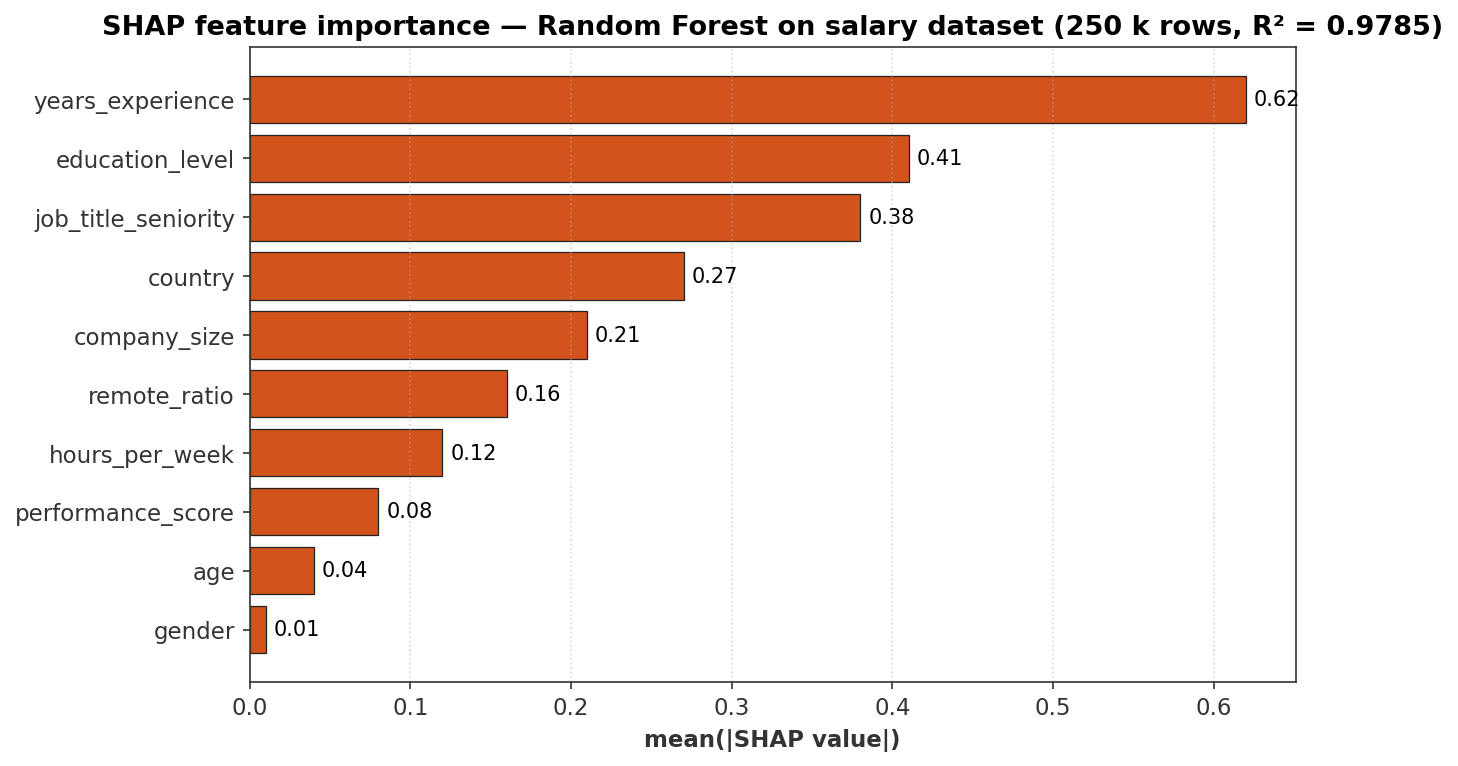
\includegraphics[width=0.85\textwidth, keepaspectratio]{diagrams/ch5_fig6}
  \caption{SHAP feature importance bar chart --- top contributors to the prediction.}
  \label{fig:ch5_fig6}
\end{figure}

\subsection{Model export}

The export step packages the trained \texttt{.joblib} artefact along
with a generated FastAPI inference script. The user downloads a zip
that they can drop onto any container runtime to serve the model
without the platform at all. That property --- being able to leave
--- mattered on principle. A no-code platform that locks a user in
is not removing friction; it is relocating it.

\subsection{Why \texttt{joblib} and not \texttt{pickle}}

\texttt{joblib} was the deliberate choice for the tabular path
because its custom pickler is optimised for objects containing large
NumPy arrays --- which every scikit-learn estimator holds --- and
can memory-map them on load. For a Random Forest of $500$ trees the
on-disk size difference was roughly $8\times$ in our measurements;
the load-time difference was larger. For the deep-learning path in
Sprint~4 we use \texttt{torch.save} on a \texttt{state\_dict()}
instead --- a different ecosystem, a different convention.

\section{Unit Tests}

\begin{itemize}
    \item Each \texttt{BaseMLModel} subclass has a happy-path test on
        a tiny fixture dataset (50 rows, four columns, a binary
        target). Assertions cover output shape and the presence of
        the documented metric keys.
    \item The algorithm-factory is exercised by parametrised tests
        --- one per algorithm string --- that construct the model,
        train, predict, and inspect the result envelope.
    \item Node validation: parametrised tests over
        (node-type, upstream-edges, expected-status) tuples.
    \item Export bundle: the generated zip is unzipped to a
        \texttt{tempdir} and the FastAPI script is imported to
        confirm it parses. The actual inference call is exercised
        by an end-to-end test in the deployment chapter.
\end{itemize}

\section*{Conclusion}

Sprint~2 was the sprint where the project first felt like a real
product. A user could open the canvas, drop three nodes, hit Run,
and watch a model train in front of them. The \texttt{BaseMLModel}
abstraction introduced here later absorbed the deep-learning
extension in Sprint~4 without disturbing the orchestration code, and
the SHAP plus export surface closed the loop between training a
model and being able to do something with it.

% ═════════════════════════════════════════════════════════════════════════════
\chapter{Sprint 3: Local Generative AI and Retrieval-Augmented Chat}
% ═════════════════════════════════════════════════════════════════════════════

\section*{Introduction}

This was the most technically ambitious sprint of the project. A
fully local Retrieval-Augmented Generation pipeline meant fitting an
embedding model, a vector store, and an LLM inside the same Docker
stack as the rest of the platform --- and making the chat experience
responsive enough that users would not notice they were running it
on a consumer GPU.

\section{Sprint Backlog}

\begin{table}[H]
\centering
\caption{Sprint~3 backlog --- local RAG.}
\label{tab:sprint3_backlog}
\begin{tabular}{@{}p{0.05\linewidth} L{0.55\linewidth} p{0.1\linewidth} p{0.18\linewidth}@{}}
\toprule
\textbf{ID} & \textbf{User Story / Task} & \textbf{Priority} & \textbf{Estimation (d)} \\
\midrule
US-21 & Document ingestion pipeline (PDF, DOCX, plain text). & High & 1 \\
US-22 & Local embedding via \texttt{sentence-transformers}. & High & 0.5 \\
US-23 & Vector store in \texttt{pgvector} (IVFFlat index). & High & 1 \\
US-24 & Ollama integration serving Llama~3.2~3B Q4\_K\_M. & High & 1 \\
US-25 & Chat orchestration --- embed, retrieve top-$k$, build prompt, stream. & High & 2 \\
US-26 & Streamed UI: tokens render as they arrive over SocketIO. & High & 1.5 \\
US-27 & RAG-mode toggle on the canvas with three node types. & Medium & 1 \\
US-28 & Source-chunks chip showing retrieved chunks + similarity. & Low & 0.5 \\
\bottomrule
\end{tabular}
\end{table}

\section{Concepts fondamentaux}

Three concepts carry the weight of this sprint; the design and
implementation sections below assume them.

\textbf{Embeddings.} A sentence-transformer maps a chunk of text to a
fixed-dimensional vector (384 dimensions for MiniLM-L6-v2) such that
cosine similarity of the vectors correlates with semantic similarity
of the text. The embedding is one-way and lossy; the vector cannot be
inverted back into the chunk.

\textbf{Vector store with approximate nearest-neighbour search.}
\texttt{pgvector}'s IVFFlat index partitions the vector space into
clusters at index-build time, then at query time visits the closest
clusters only. For the local-tenant scale this project targets, the
recall/latency trade-off lands firmly on the latency side --- under
$50$\,ms for top-$k$ over a few hundred thousand chunks.

\textbf{Retrieval-Augmented Generation.} Rather than fine-tuning a
model on the user's documents, the pipeline retrieves the top-$k$
most similar chunks at query time and concatenates them into the
prompt as context. The model is instructed to answer from the
provided context and to refuse rather than guess. This trades a
training step for a retrieval step --- the right trade when the
corpus changes faster than a fine-tune can keep up with.

\section{Design}

\begin{figure}[H]
  \centering
  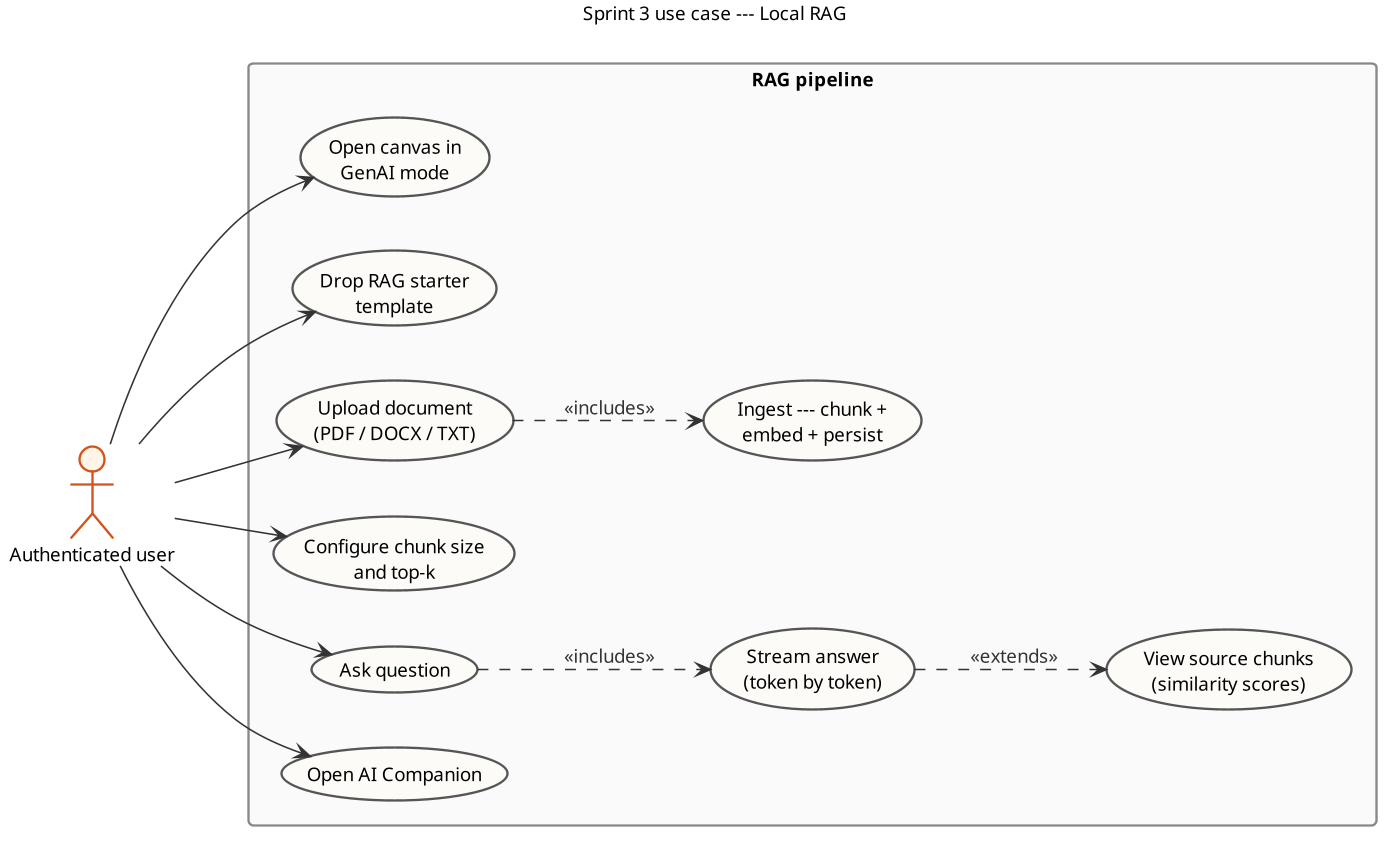
\includegraphics[width=0.85\textwidth, keepaspectratio]{diagrams/ch6_fig1}
  \caption{Use case diagram --- RAG pipeline.}
  \label{fig:ch6_fig1}
\end{figure}

\begin{figure}[H]
  \centering
  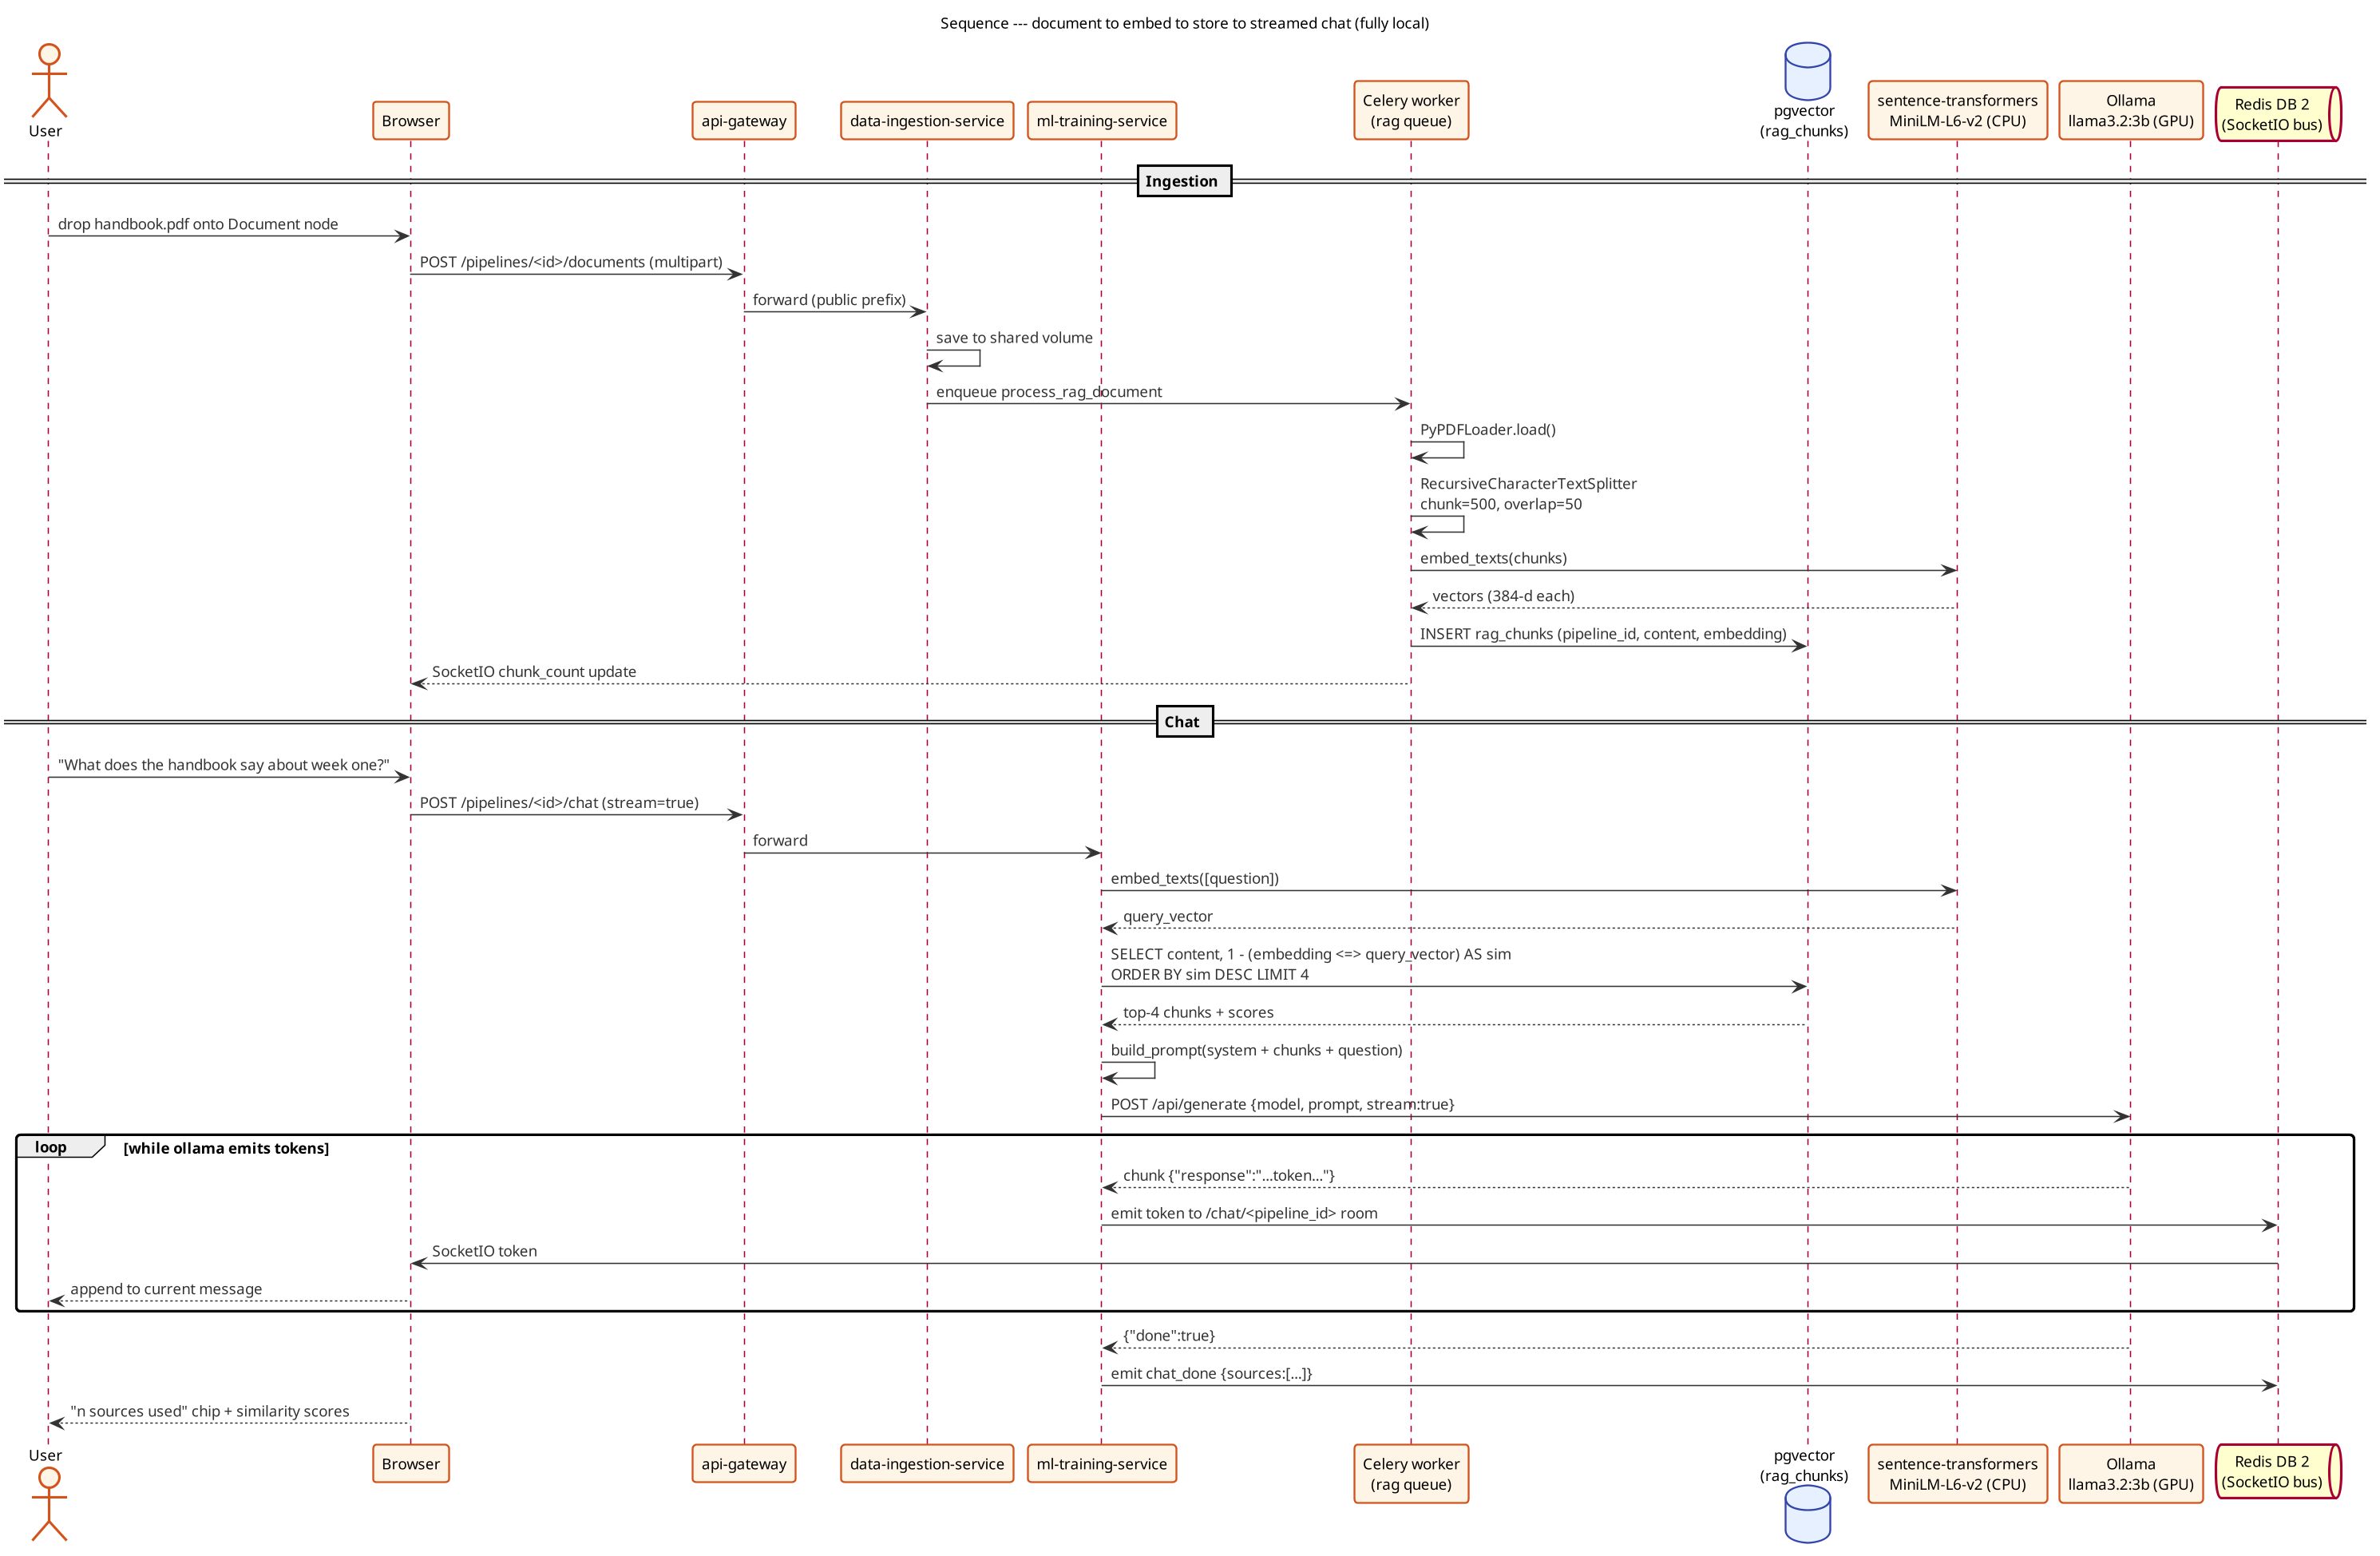
\includegraphics[width=0.85\textwidth, keepaspectratio]{diagrams/ch6_fig2}
  \caption{Sequence diagram --- document to embed to store to chat.}
  \label{fig:ch6_fig2}
\end{figure}

\begin{figure}[H]
  \centering
  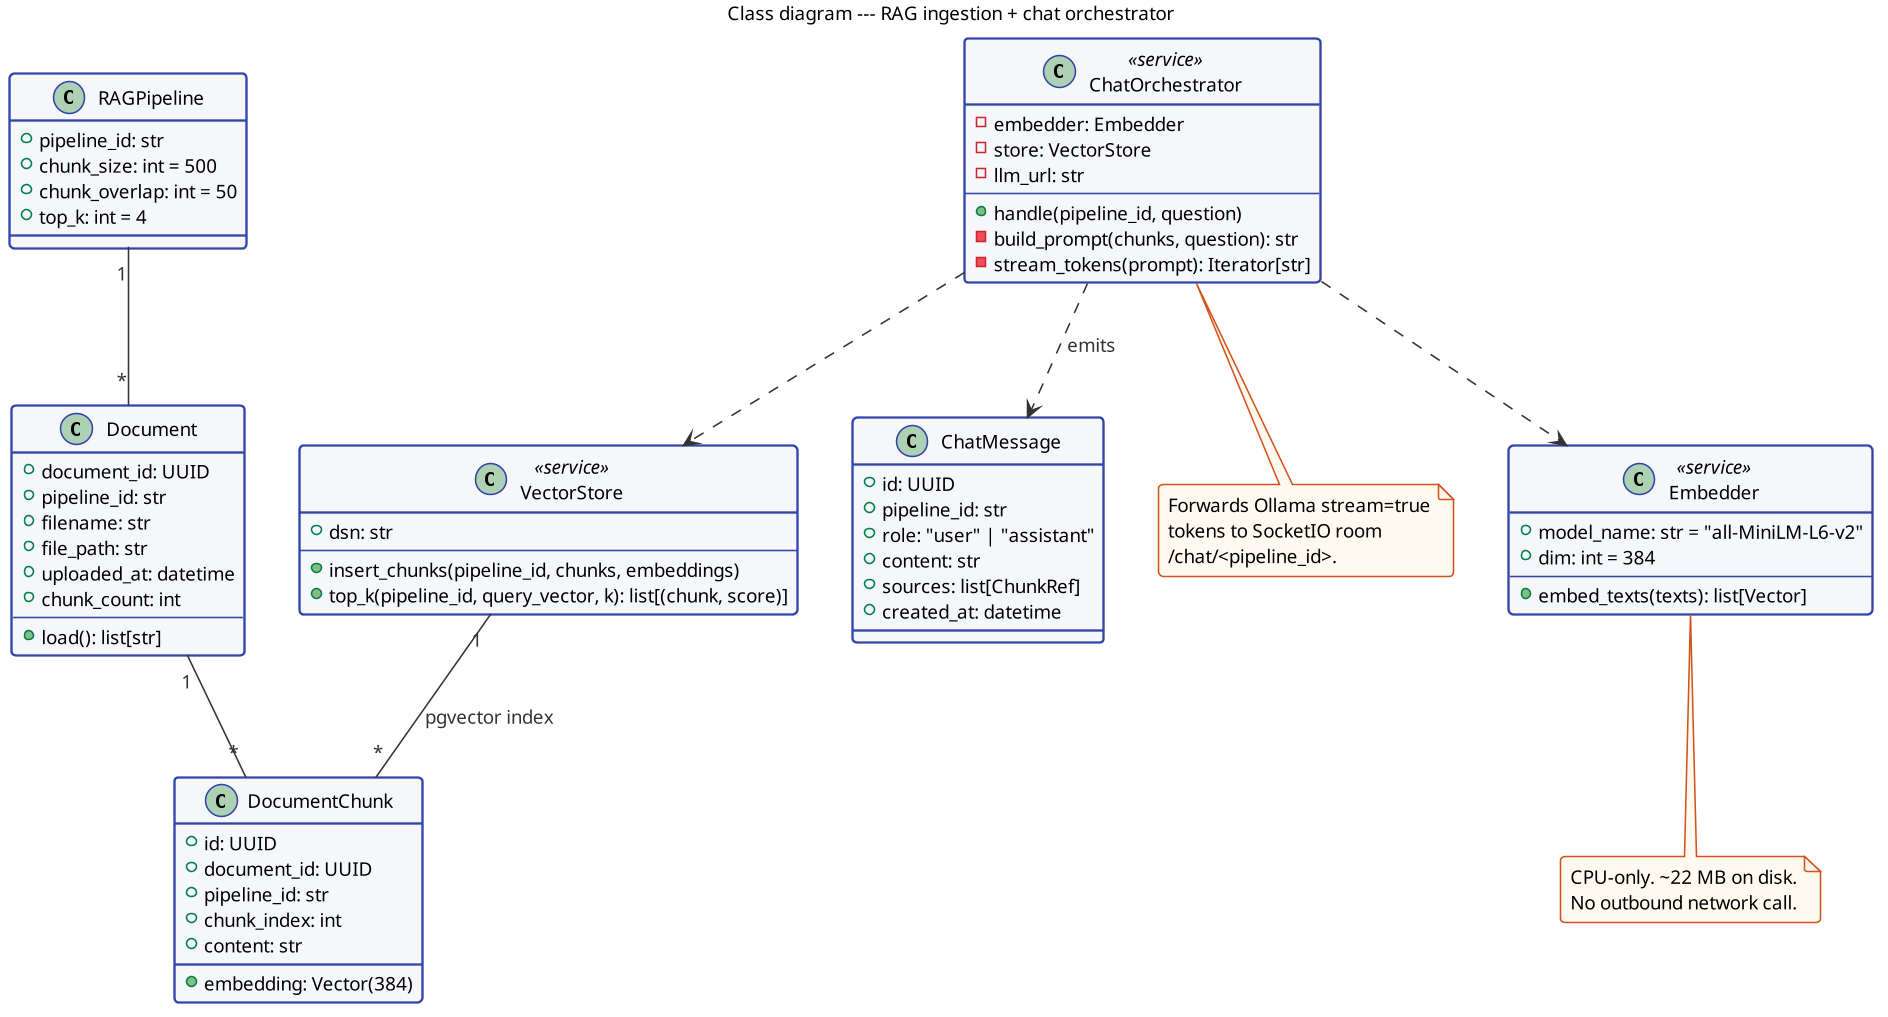
\includegraphics[width=0.85\textwidth, keepaspectratio]{diagrams/ch6_fig3}
  \caption{Class diagram --- RAG ingestion plus chat orchestrator.}
  \label{fig:ch6_fig3}
\end{figure}

A Retrieval-Augmented Generation pipeline grounds a language model in
documents the user provides. The pipeline embeds each document chunk
into a vector, stores those vectors in a database that supports
similarity search, and at query time embeds the question, retrieves
the most similar chunks, and concatenates them into the model's
prompt as context. The model then answers from the retrieved
content, which keeps responses grounded in the source documents and
sidesteps the hallucination patterns that pure-LLM chat is prone to.

The component picks for this project:

\begin{itemize}
    \item \textbf{\texttt{sentence-transformers/all-MiniLM-L6-v2}}
        for embeddings. The model is small (around $22$\,MB on
        disk, 384 output dimensions), runs fast on CPU, and produces
        embeddings whose cosine similarity correlates well with
        semantic similarity in English and reasonably well in French.
        Larger models (\texttt{all-mpnet-base-v2}, OpenAI's
        \texttt{text-embedding-3-small}) would lift retrieval quality
        a few points but cost CPU latency and, in the OpenAI case,
        violate the data-sovereignty constraint outright.
    \item \textbf{\texttt{pgvector}} for the vector store, with an
        IVFFlat index. Co-locating the store in the auth-service
        Postgres instance avoided spinning up a sixth backing
        service. IVFFlat trades a small amount of recall for a
        large gain in query latency, which is the right trade for
        a few hundred thousand chunks per tenant.
    \item \textbf{Ollama running \texttt{llama3.2:3b}} as the LLM
        engine. \texttt{Q4\_K\_M} quantisation fits in roughly
        $2$\,GB of VRAM, which leaves headroom on the 6\,GB demo GPU
        for embeddings, canvas, and the training queue to share the
        same device without stepping on each other.
\end{itemize}

\section{Implementation}

\begin{lstlisting}[language=Python, caption=Document ingestion task (\texttt{ml-training-service/app/tasks/rag\_ingest.py})]
@celery.task(name="app.tasks.rag_ingest.process_rag_document", bind=True)
def process_rag_document(self, document_id, pipeline_id, file_path):
    from langchain_text_splitters import RecursiveCharacterTextSplitter
    from langchain_community.document_loaders import PyPDFLoader

    docs = PyPDFLoader(file_path).load()
    splitter = RecursiveCharacterTextSplitter(
        chunk_size=500, chunk_overlap=50, length_function=len,
    )
    split_docs = splitter.split_documents(docs)
    chunk_texts = [d.page_content for d in split_docs if d.page_content.strip()]

    # Local embedding via sentence-transformers — no network call.
    vectors = embed_texts(chunk_texts)
    insert_chunks(
        pipeline_id=pipeline_id,
        document_id=document_id,
        chunks=chunk_texts,
        embeddings=vectors,
    )
\end{lstlisting}

\subsection{Streamed chat}

The chat response streams token by token over SocketIO. The
\texttt{ml-training-service} acts as producer: it embeds the
question, queries pgvector for the top-$k$ chunks (default $k=4$),
builds the prompt with the retrieved context, and forwards Ollama's
\texttt{stream=true} chunks straight into the
\texttt{/chat/<pipeline\_id>} room. The frontend appends each token
to the current assistant message as it arrives. The first time that
worked end-to-end --- on a laptop, with no network involved --- was
the moment the project's thesis stopped feeling speculative.

\begin{figure}[H]
  \centering
  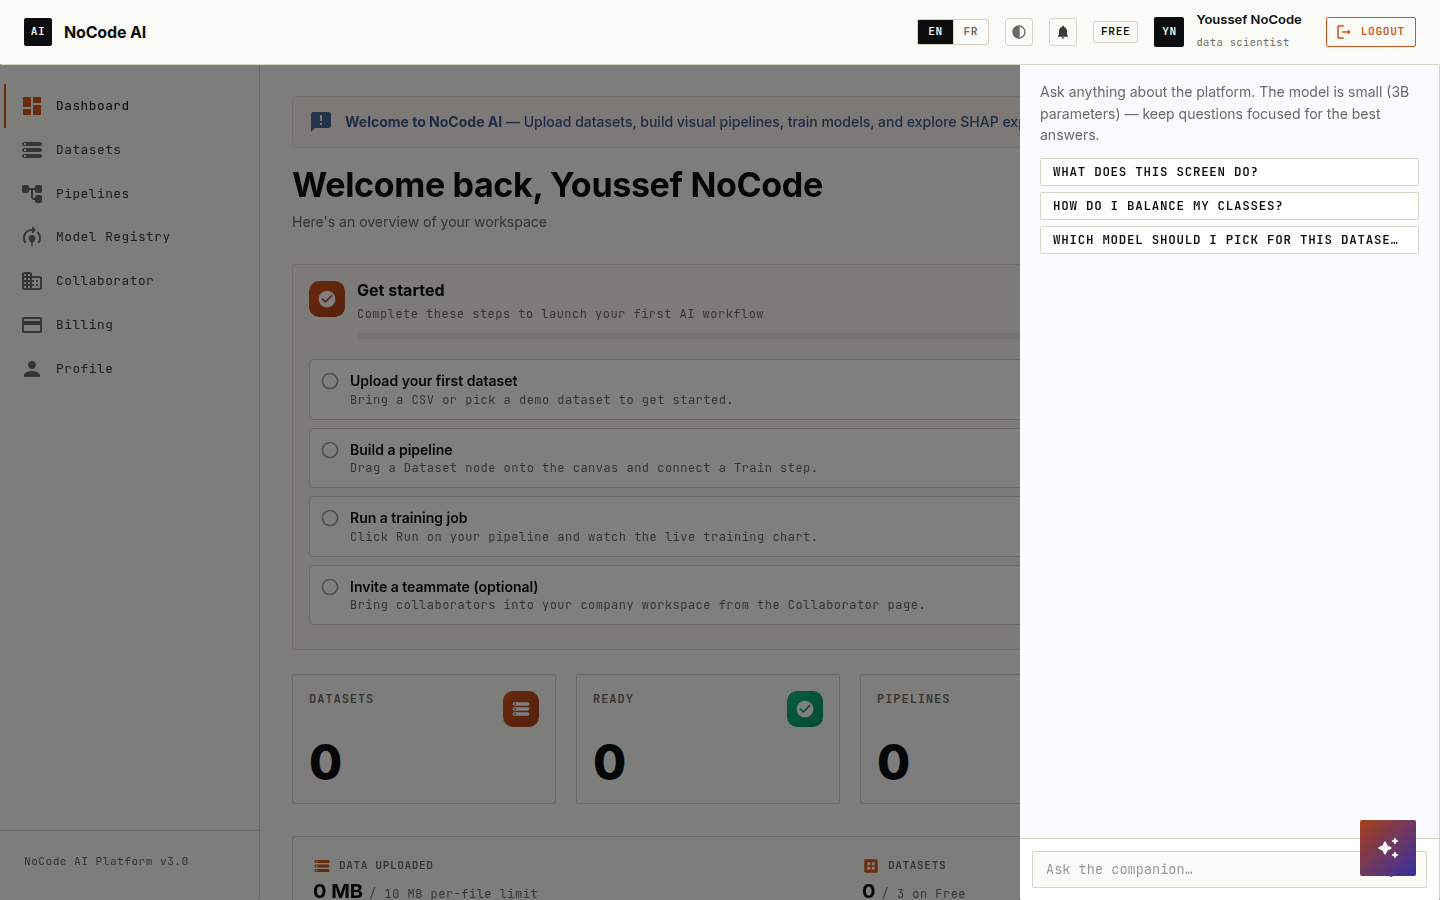
\includegraphics[width=0.85\textwidth, keepaspectratio]{diagrams/ch6_fig4}
  \caption{RAG chat panel --- tokens stream in as the model emits them.}
  \label{fig:ch6_fig4}
\end{figure}

\subsection{Chunk sizing trade-offs}

Five hundred characters with a fifty-character overlap is the
default chunking. We tested shorter chunks (256, 128) and longer
ones (1024). Short chunks raised retrieval precision on single-fact
questions but ruined it for anything that needed multi-sentence
context; long chunks did the opposite, packing too much unrelated
material into each retrieval slot. Five hundred sat in the middle.
It is a defensible default, not a universal answer; the backlog
notes a follow-up to expose chunk size as a per-pipeline setting
once the platform has enough usage data to choose by document type
automatically.

\subsection{Prompt construction}

The system prompt instructs the model to answer from the retrieved
context and to refuse rather than guess if the context does not
cover the question. The retrieved chunks are inserted in similarity
order, each prefixed with a document identifier so the model can
cite. The user-facing chip ``$n$ sources used'' lists the chunks and
their cosine similarity scores, which gives the reader a way to
verify the answer against the original source --- the closest thing
to accountability that a generative system can offer.

\section{Unit Tests}

\begin{itemize}
    \item Chunking determinism --- the same input file produces the
        same chunks across runs.
    \item Embedding shape --- 384 dimensions, normalised.
    \item Retrieval top-$k$ on a deterministic five-chunk corpus
        with hand-labelled relevance.
    \item Chat orchestrator: Ollama is mocked at the HTTP boundary,
        the orchestrator is asserted to emit the right SocketIO
        events in the right order.
\end{itemize}

The Ollama process itself is not exercised in unit tests --- it sits
behind the smoke-test script in the deployment chapter.

\section*{Conclusion}

Sprint~3 proved the local-generative-AI thesis. The chat is not as
fast as GPT-4 over the wire, and it never will be on this hardware,
but it is interactive enough to be useful and it keeps the user's
documents on the user's machine. For the regulated audiences this
project is framed against, that trade-off is the right one.

% ═════════════════════════════════════════════════════════════════════════════
\chapter{Sprint 4: Deep Learning for Image Classification}
% ═════════════════════════════════════════════════════════════════════════════

\section*{Introduction}

This sprint added the third pipeline mode. Deep learning on the demo
hardware is a constrained problem --- 6\,GB of VRAM does not forgive
carelessness --- so the design started from the constraint and
worked backwards. The result is a small, opinionated catalogue
rather than a kitchen-sink layer builder, and the opinionation is
the feature.

\section{Sprint Backlog}

\begin{table}[H]
\centering
\caption{Sprint~4 backlog --- deep learning for image classification.}
\label{tab:sprint4_backlog}
\begin{tabular}{@{}p{0.05\linewidth} L{0.55\linewidth} p{0.1\linewidth} p{0.18\linewidth}@{}}
\toprule
\textbf{ID} & \textbf{User Story / Task} & \textbf{Priority} & \textbf{Estimation (d)} \\
\midrule
US-29 & New microservice: \texttt{dl-training-service}. & High & 1 \\
US-30 & Three CNN architectures (LeNet, ResNet-9, MobileNet-V3-Small). & High & 2 \\
US-31 & Image-dataset ingestion (zip of \texttt{<class>/<file>}). & High & 1 \\
US-32 & Static VRAM estimator (the VRAM guard). & High & 2 \\
US-33 & Tier-aware ceilings on epochs and batch size. & High & 0.5 \\
US-34 & Live training visualisation (reused from Sprint~2). & Medium & 0.5 \\
US-35 & Inline single-image inference (the ``Try it'' panel). & Medium & 1 \\
US-36 & DL-mode canvas toggle with three new node components. & Medium & 1.5 \\
\bottomrule
\end{tabular}
\end{table}

\section{Concepts fondamentaux}

\textbf{Convolutional layers.} A 2D convolution slides a small
trainable kernel across the input image, producing a feature map
that responds to local patterns (edges, textures, shapes). Stacking
several convolution + pooling layers builds a hierarchy from
low-level features to class-discriminative ones.

\textbf{Residual connections.} A residual block adds the block's
input to its output, so a layer learns the residual mapping
$F(x) + x$ rather than $F(x)$ alone. This eases gradient flow in
deeper networks and is the reason the custom ResNet-9 trains
predictably even on small datasets.

\textbf{Transfer learning.} Loading a model with weights already
trained on ImageNet, then fine-tuning the final layers on the
user's dataset. For 200-image custom datasets the transfer-learned
MobileNet-V3 reaches usable accuracy in minutes; a random-init run
on the same data takes an order of magnitude longer.

\textbf{Batch normalisation and the optimiser memory footprint.}
Adam keeps two moment estimates per parameter (mean and variance),
which doubles the optimiser-state memory compared to plain SGD.
This factor is the dominant term in the VRAM guard's static estimate
documented below.

\section{Design}

\begin{figure}[H]
  \centering
  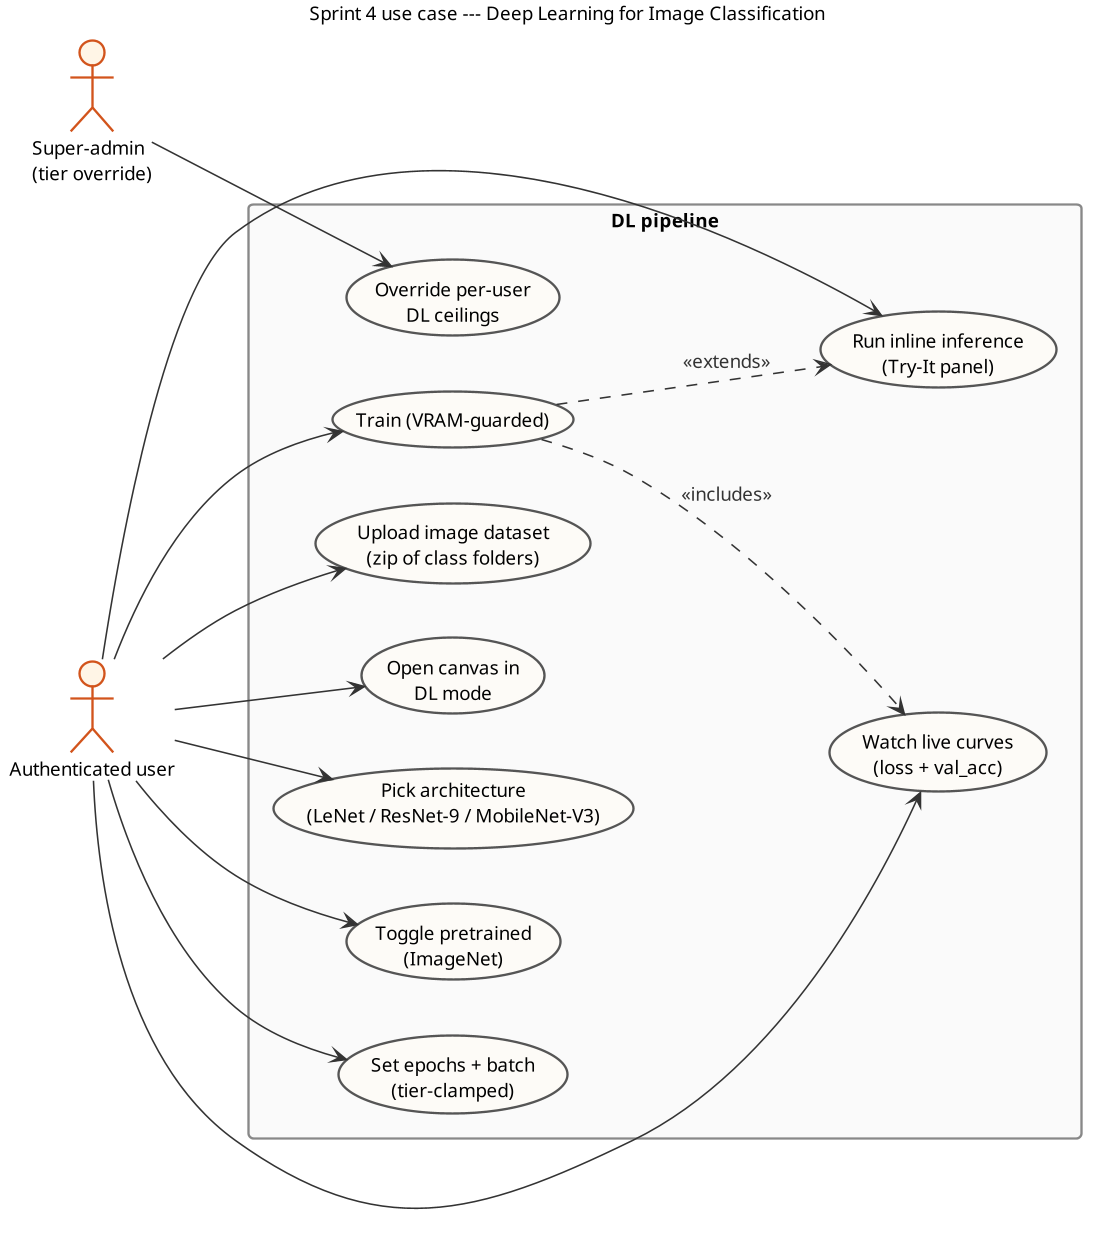
\includegraphics[width=0.85\textwidth, keepaspectratio]{diagrams/ch7_fig1}
  \caption{Use case diagram --- DL pipeline.}
  \label{fig:ch7_fig1}
\end{figure}

\begin{landscape}
\begin{figure}[H]
  \centering
  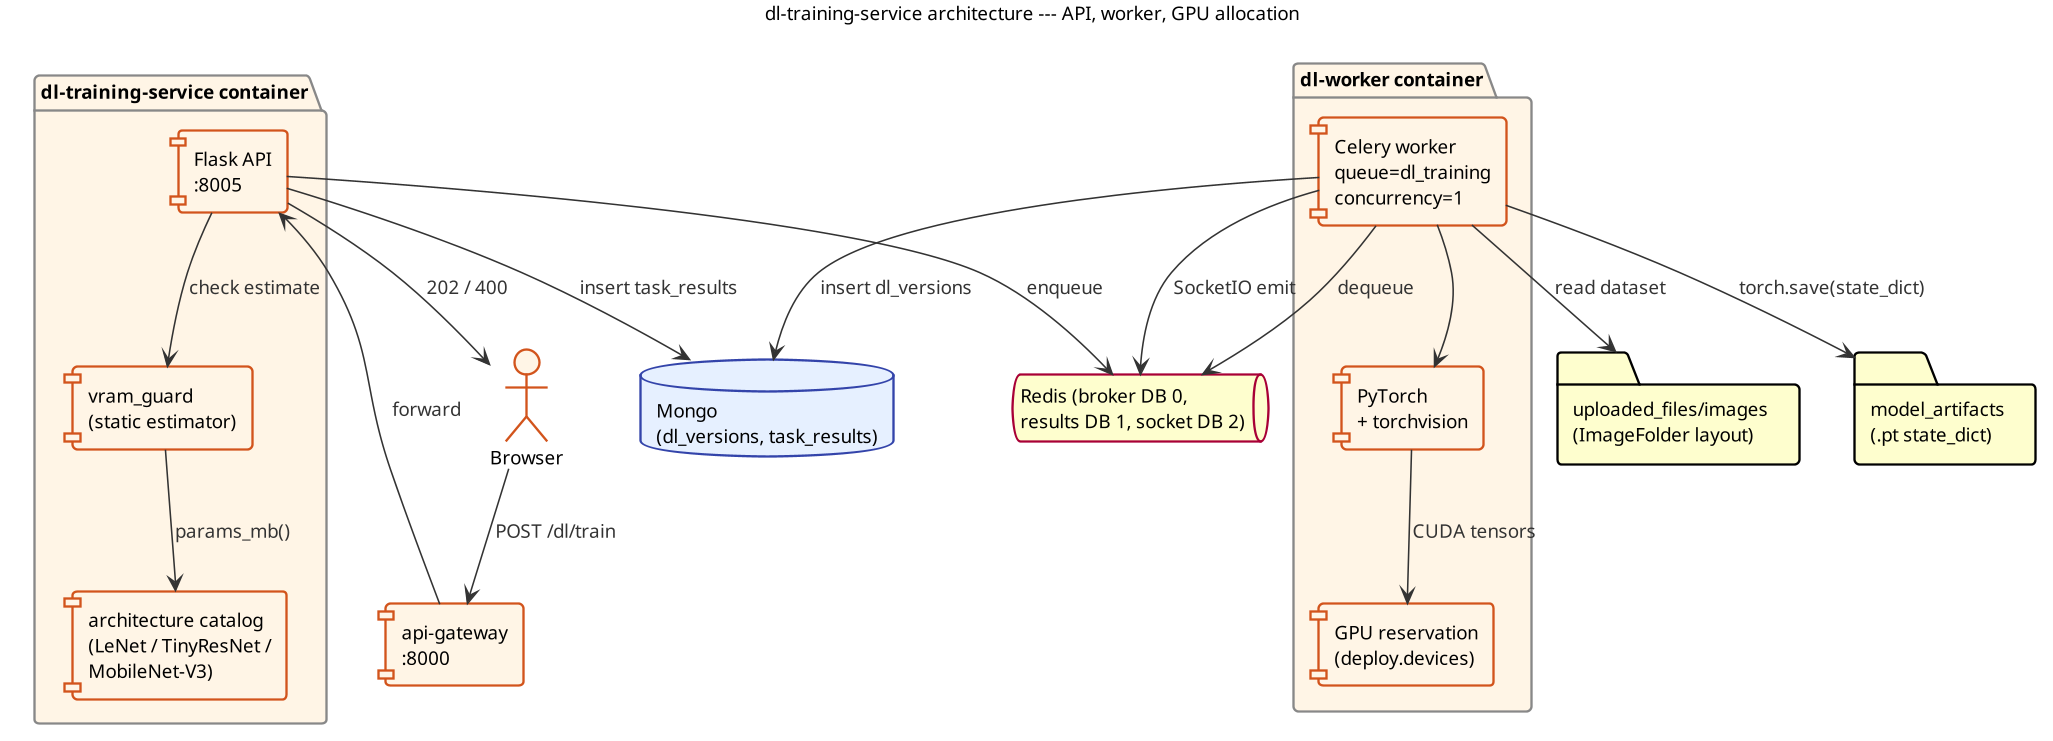
\includegraphics[width=0.95\linewidth, keepaspectratio]{diagrams/ch7_fig2}
  \caption{Architecture --- \texttt{dl-training-service}, Celery worker, GPU allocation.}
  \label{fig:ch7_fig2}
\end{figure}
\end{landscape}

\begin{figure}[H]
  \centering
  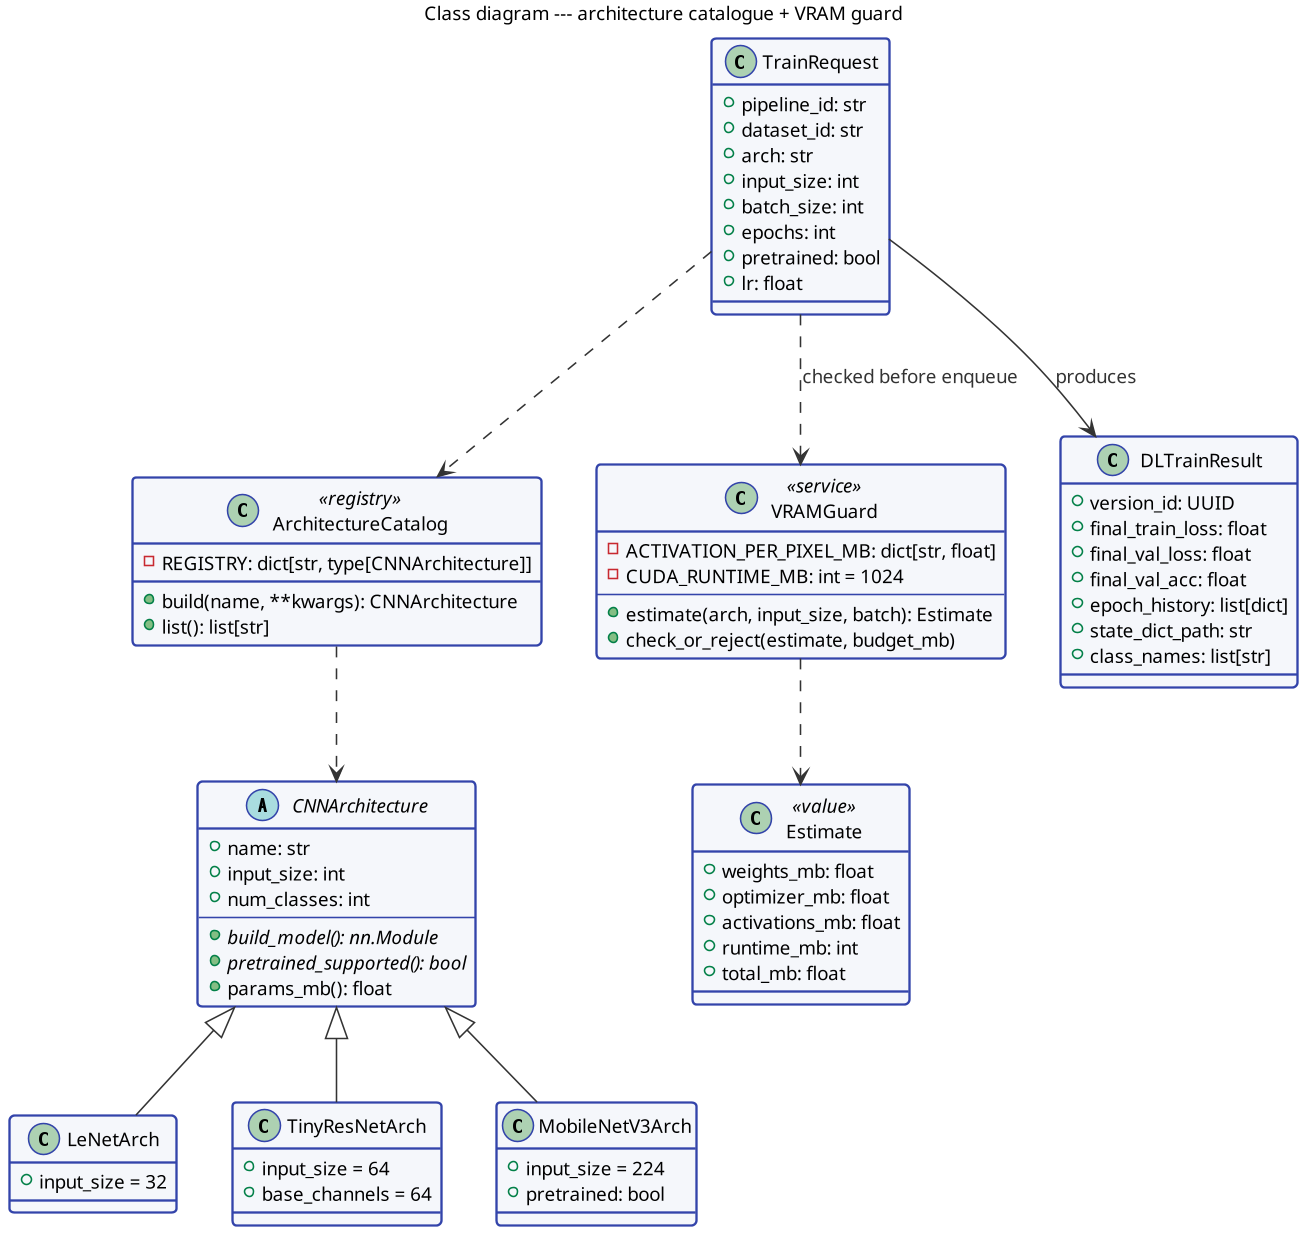
\includegraphics[width=0.85\textwidth, keepaspectratio]{diagrams/ch7_fig3}
  \caption{Class diagram --- architecture catalogue plus VRAM guard.}
  \label{fig:ch7_fig3}
\end{figure}

\begin{figure}[H]
  \centering
  \begin{subfigure}{0.95\textwidth}
    \centering
    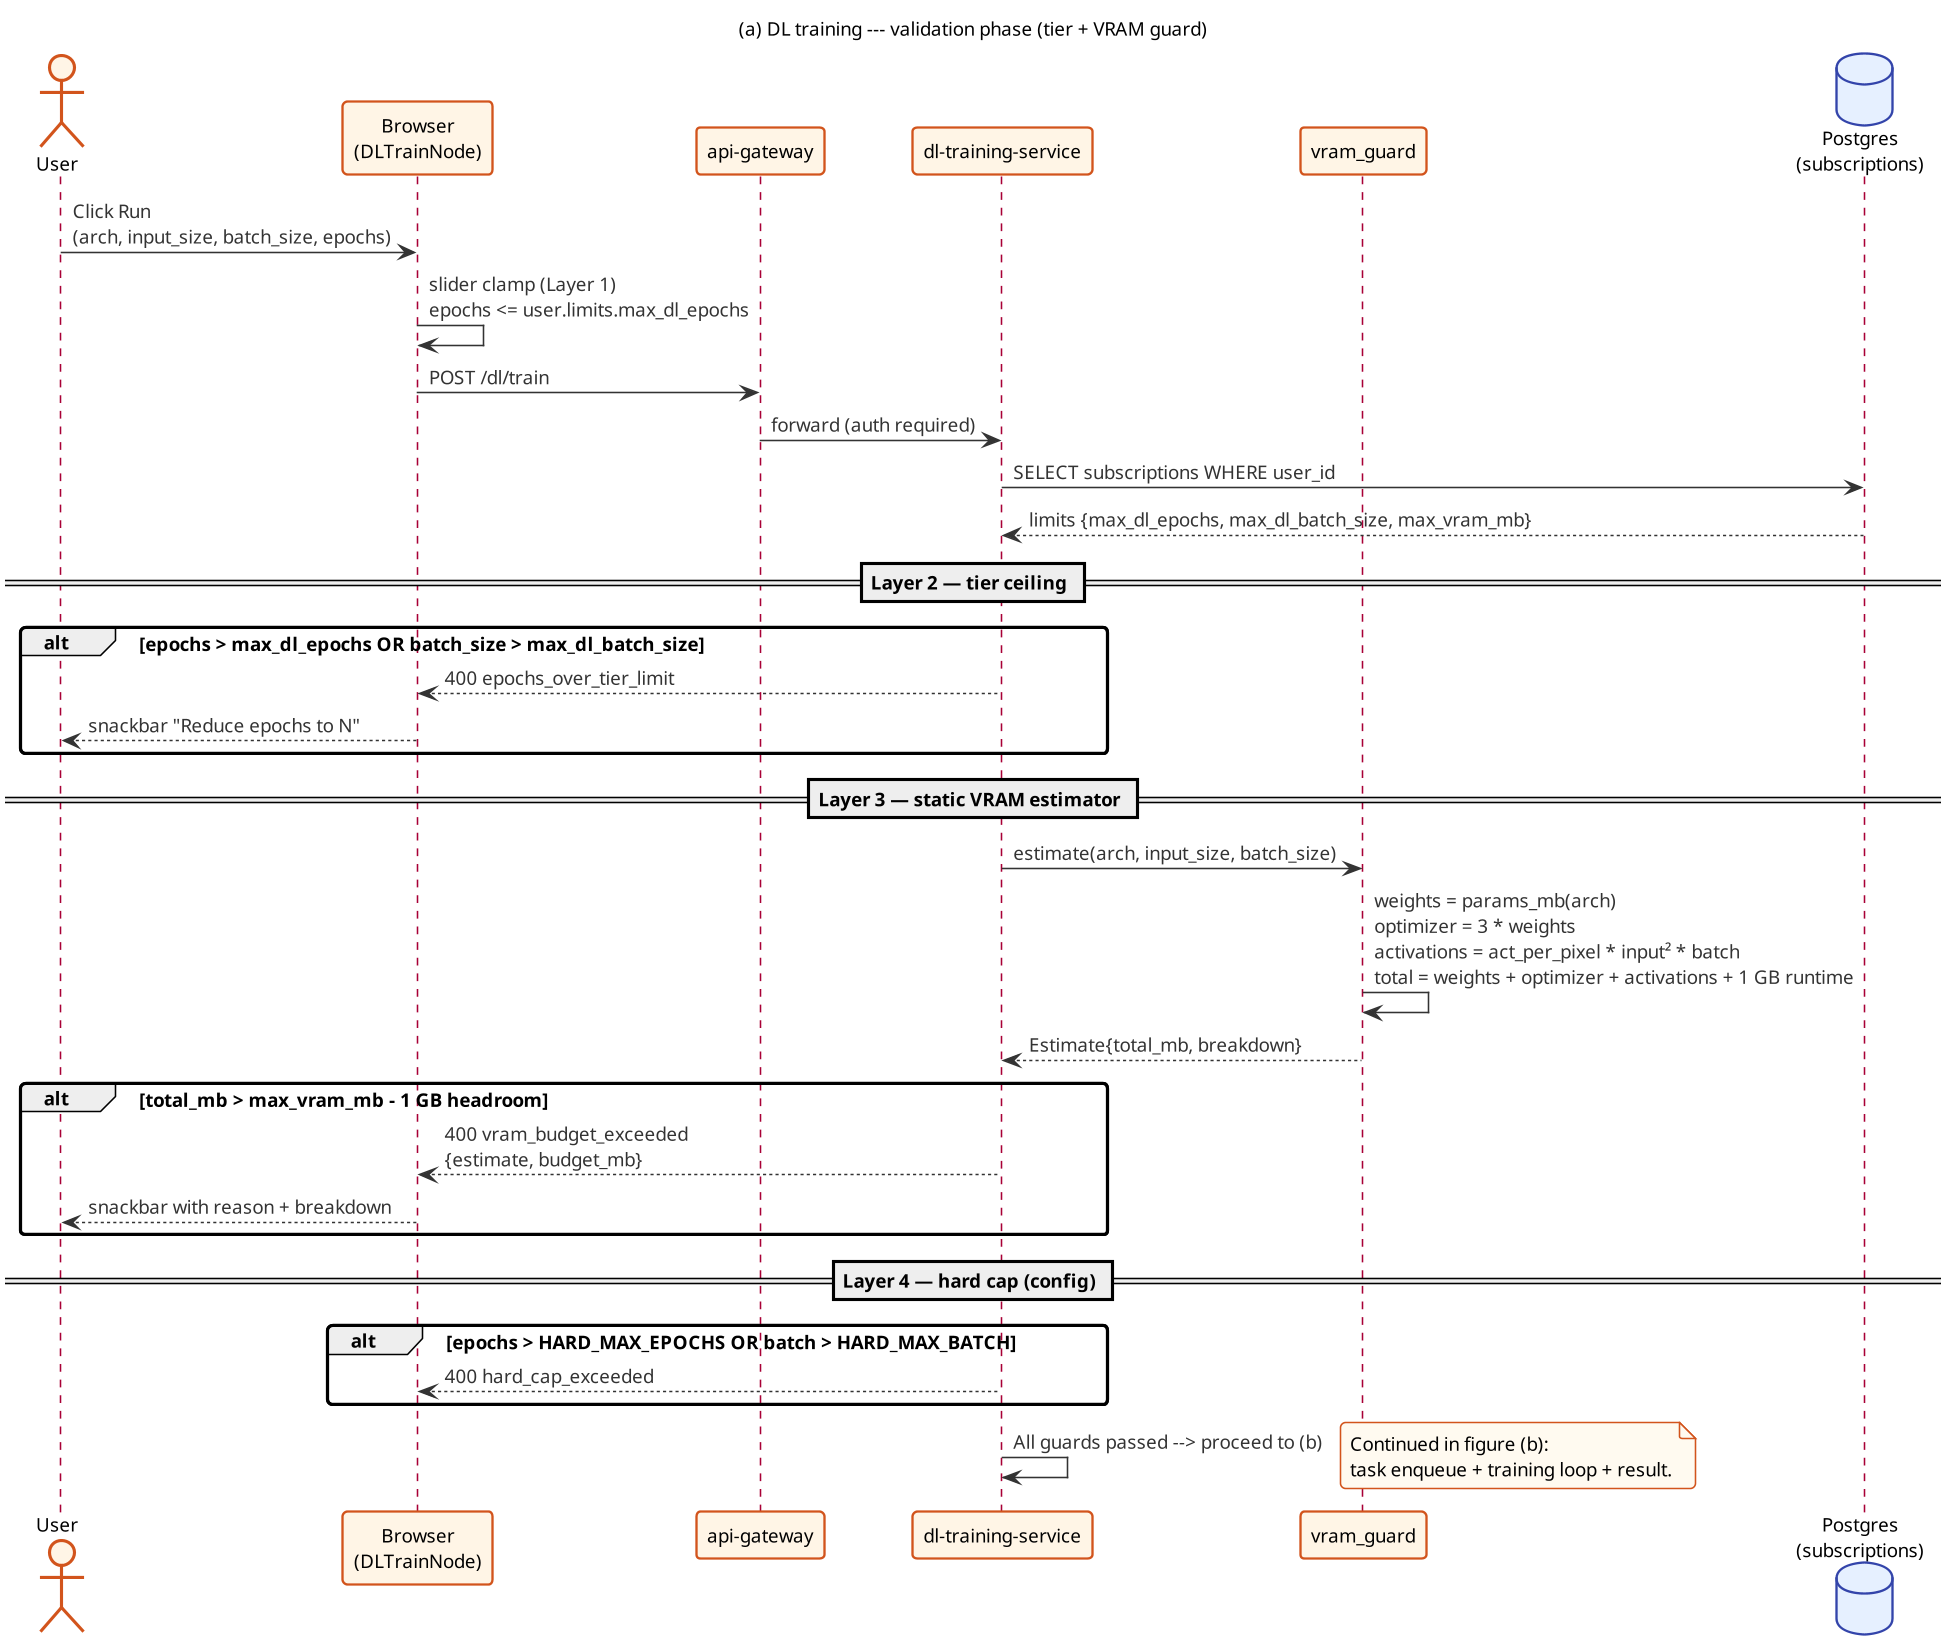
\includegraphics[width=\linewidth]{diagrams/ch7_fig_seq_training_a}
    \caption{Validation phase --- tier ceiling + VRAM guard. Rejection branches return 400 before any GPU work happens.}
    \label{fig:ch7_fig_seq_training_a}
  \end{subfigure}
  \vspace{6pt}
  \begin{subfigure}{0.95\textwidth}
    \centering
    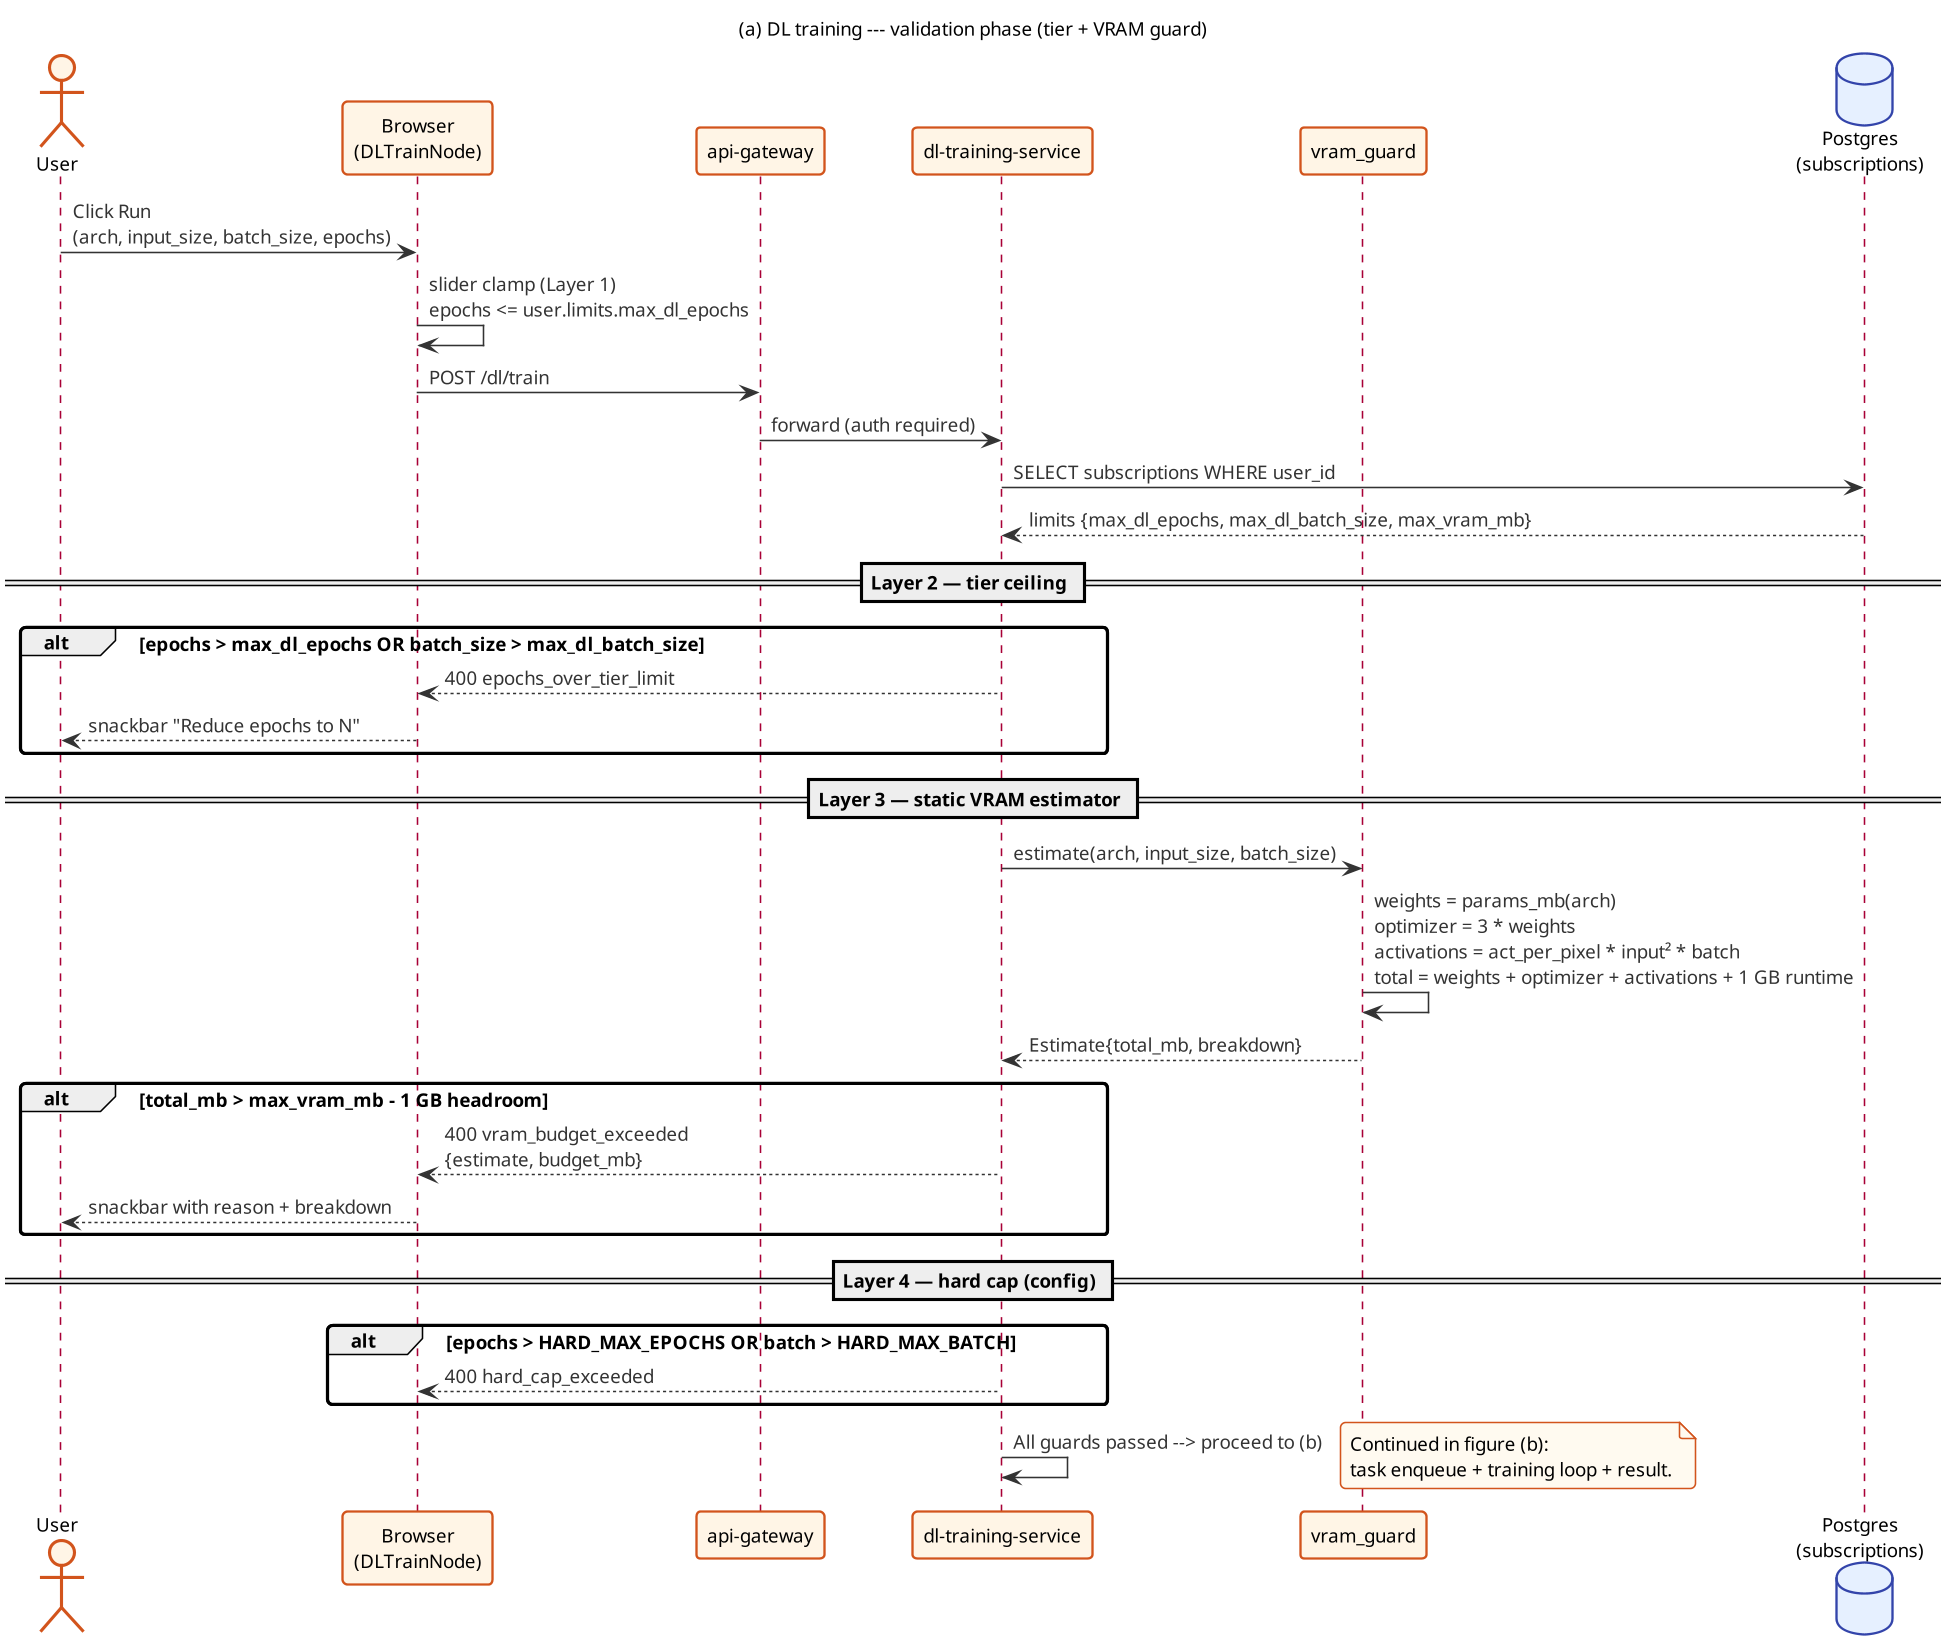
\includegraphics[width=\linewidth]{diagrams/ch7_fig_seq_training_a}
    \caption{Training phase --- only reached when validation succeeds; epochs stream over SocketIO.}
    \label{fig:ch7_fig_seq_training_b}
  \end{subfigure}
  \caption{Sequence diagram --- DL training flow, split into (a) validation and (b) training phases.}
  \label{fig:ch7_fig_seq_training}
\end{figure}

\subsection{Scope decisions}

What stayed in:

\begin{itemize}
    \item Three architectures: LeNet (smoke-test scale), a custom
        ResNet-9 (\textit{tiny\_resnet}), and torchvision's
        MobileNet-V3-Small with optional ImageNet transfer
        learning.
    \item Image-dataset upload: a zip of \texttt{<class>/<file>}
        folders, extracted into the canonical \texttt{ImageFolder}
        layout that PyTorch's data loaders expect.
    \item Live training visualisation reused from the tabular path
        (the \texttt{training\_epoch} socket event fans out into
        train/val loss and val-accuracy series).
    \item Single-image inference (the ``Try it'' panel) inline
        immediately after training completes.
\end{itemize}

What stayed out, deliberately:

\begin{itemize}
    \item Freeform layer-builder DAG --- too easy for the user to
        configure something that does not fit.
    \item LLM fine-tuning --- won't fit inside 6\,GB.
    \item Object detection and segmentation --- different label
        format, different demo, different scope.
    \item ONNX export --- a one-file follow-up if needed, not in
        scope.
    \item Multi-GPU and distributed training.
\end{itemize}

Drawing this line clearly mattered as much as anything we built. A
no-code deep-learning interface that lets the user wire up an
architecture that doesn't fit is, in practice, a debugger the user
did not ask for.

\subsection{Why CNN architectures, and which three}

The image-classification problem on small custom datasets
(hundreds, not millions, of labelled images) favours convolutional
networks over transformer-based vision models. Vision Transformers
need orders of magnitude more data or aggressive pretraining to
match a competent CNN's accuracy, and the demo budget does not
support either. The three architectures in the catalogue were chosen
to span three operating points.

\textbf{LeNet} (roughly $60$\,k parameters) is the smoke-test
architecture. It trains in seconds on Fashion-MNIST-class data and
serves as the smallest credible CNN --- useful for verifying the
training path end-to-end before committing to a longer run.

\textbf{Tiny ResNet} (a custom ResNet-9, roughly $2.7$\,M parameters)
is the workhorse. Two residual blocks with channels
$64 \to 128 \to 256$, skip connections that ease gradient flow, and
batch normalisation throughout. The architecture reaches around
$90\%$ accuracy on CIFAR-10 in five epochs at batch~64, input
$64$\,px --- a defensible accuracy/time trade-off for an on-stage
demo.

\textbf{MobileNet-V3-Small} (roughly $2.5$\,M parameters) is the
transfer-learning option. Loaded from torchvision with ImageNet
weights, the architecture's depthwise-separable convolutions keep
the inference cost low while the pretrained features carry most of
the work on small custom datasets. A fresh 200-image dataset can
reach $80\%$+ accuracy in two minutes; random-init would take
twenty.

\begin{table}[H]
\centering
\caption{CNN architecture catalogue with operating envelope.}
\label{tab:cnn_catalog}
\begin{tabular}{@{}L{0.21\linewidth} L{0.12\linewidth} L{0.16\linewidth} L{0.42\linewidth}@{}}
\toprule
\textbf{Architecture} & \textbf{Params} & \textbf{Demo VRAM} & \textbf{Operating point} \\
\midrule
LeNet & $\sim$60\,k & $<$0.3\,GB & Smoke-test scale. Confirms the training path end-to-end before committing to a longer run. \\
Tiny ResNet-9 & $\sim$2.7\,M & $\sim$1.5\,GB at 64\,px batch 32 & Workhorse. Hits $\sim$90\% on CIFAR-10 in five epochs; the demo default. \\
MobileNet-V3-Small & $\sim$2.5\,M & $\sim$2.0\,GB at 224\,px batch 16 & Transfer learning from ImageNet. Reaches $80\%$+ on a 200-image custom dataset in two minutes. \\
\bottomrule
\end{tabular}
\end{table}

\subsection{Why a separate microservice}

Two reasons.

First, \texttt{torch} plus \texttt{torchvision} add about $2$\,GB of
dependencies that the existing H2O-based
\texttt{ml-training-service} does not need. Co-locating them would
have doubled the size of an image that rebuilds on every CI run.

Second, GPU access is per-container in Docker. The DL service
declares a \texttt{deploy.resources.reservations.devices} block; the
H2O service runs on CPU. Mixing them in one container would either
deny GPU to the DL workload or force the H2O workload onto a GPU it
cannot use.

The service has its own Celery queue (\texttt{dl\_training}) so a
20-epoch CIFAR run cannot starve the fast tabular queue.

\section{Implementation}

\subsection{Preprocessing and augmentation}

Image tensors are resized to the architecture's expected input,
normalised to ImageNet statistics when transfer learning is enabled,
and augmented at train time with random horizontal flips and small
rotations. Augmentation is intentionally conservative: heavier
recipes (CutMix, MixUp) help on large datasets and hurt on small
ones, and small datasets are the common case here.

\subsection{The VRAM guard}

The most subtle piece of Sprint~4 is the static memory estimator:

\begin{lstlisting}[language=Python, caption=Static VRAM estimate (\texttt{dl-training-service/app/services/vram\_guard.py})]
def estimate(arch: str, input_size: int, batch_size: int) -> Estimate:
    weights = params_mb(arch)
    optimizer = 3.0 * weights              # weights + grads + 2 Adam moments
    activations = (
        _ACTIVATION_PER_PIXEL_MB[arch]
        * (input_size * input_size)
        * batch_size
    )
    total = weights + optimizer + activations + _CUDA_RUNTIME_MB
    return Estimate(weights_mb=weights, optimizer_mb=optimizer,
                    activations_mb=activations,
                    runtime_mb=_CUDA_RUNTIME_MB, total_mb=total)
\end{lstlisting}

The route refuses any \texttt{/dl/train} request whose estimate
exceeds the user's tier-resolved budget minus a $1$\,GB headroom for
the CUDA runtime and allocator fragmentation. This is the single
most important demo-safety net in the system: a wrong batch-size
press cannot OOM the GPU on stage.

The constants in \texttt{\_ACTIVATION\_PER\_PIXEL\_MB} are
conservative empirical estimates. The unit-test suite enforces that
every \texttt{(arch, input\_size, batch\_size)} triple in the
documented catalogue fits on a 6\,GB card after headroom, but it
does not pin the absolute numbers --- those drift slightly between
GPU generations and need recalibration on first deploy.

\subsection{Tier-aware ceilings}

Sprint~4 added two per-tier columns to the \texttt{subscriptions}
table: \texttt{max\_dl\_epochs} and \texttt{max\_dl\_batch\_size}.
The defaults: Free at 5 epochs / batch 32, Solo at 20 epochs / batch
64, Company at 50 epochs / batch 64.

The defence-in-depth chain runs:

\begin{enumerate}
    \item The frontend's \texttt{DLTrainNode} reads the user's
        \texttt{limits} from \texttt{/users/me} and clamps the
        slider \texttt{max} accordingly --- a free-tier user
        literally cannot select 20 epochs from the UI.
    \item The route enforces the tier ceiling regardless: a custom
        client posting 50 epochs to \texttt{/dl/train} on a
        free-tier token receives \texttt{400 epochs\_over\_tier\_limit}.
    \item The \texttt{vram\_guard} then checks the static memory
        estimate against the tier's VRAM budget.
    \item The service-wide \texttt{HARD\_MAX\_EPOCHS} and
        \texttt{HARD\_MAX\_BATCH\_SIZE} caps in \texttt{config.py}
        sit as an absolute ceiling that no tier override can lift.
\end{enumerate}

Four layers may sound paranoid, but each one catches a different
class of mistake --- accidental, malicious, oversized, pathological
--- and none of them is expensive.

\begin{figure}[H]
  \centering
  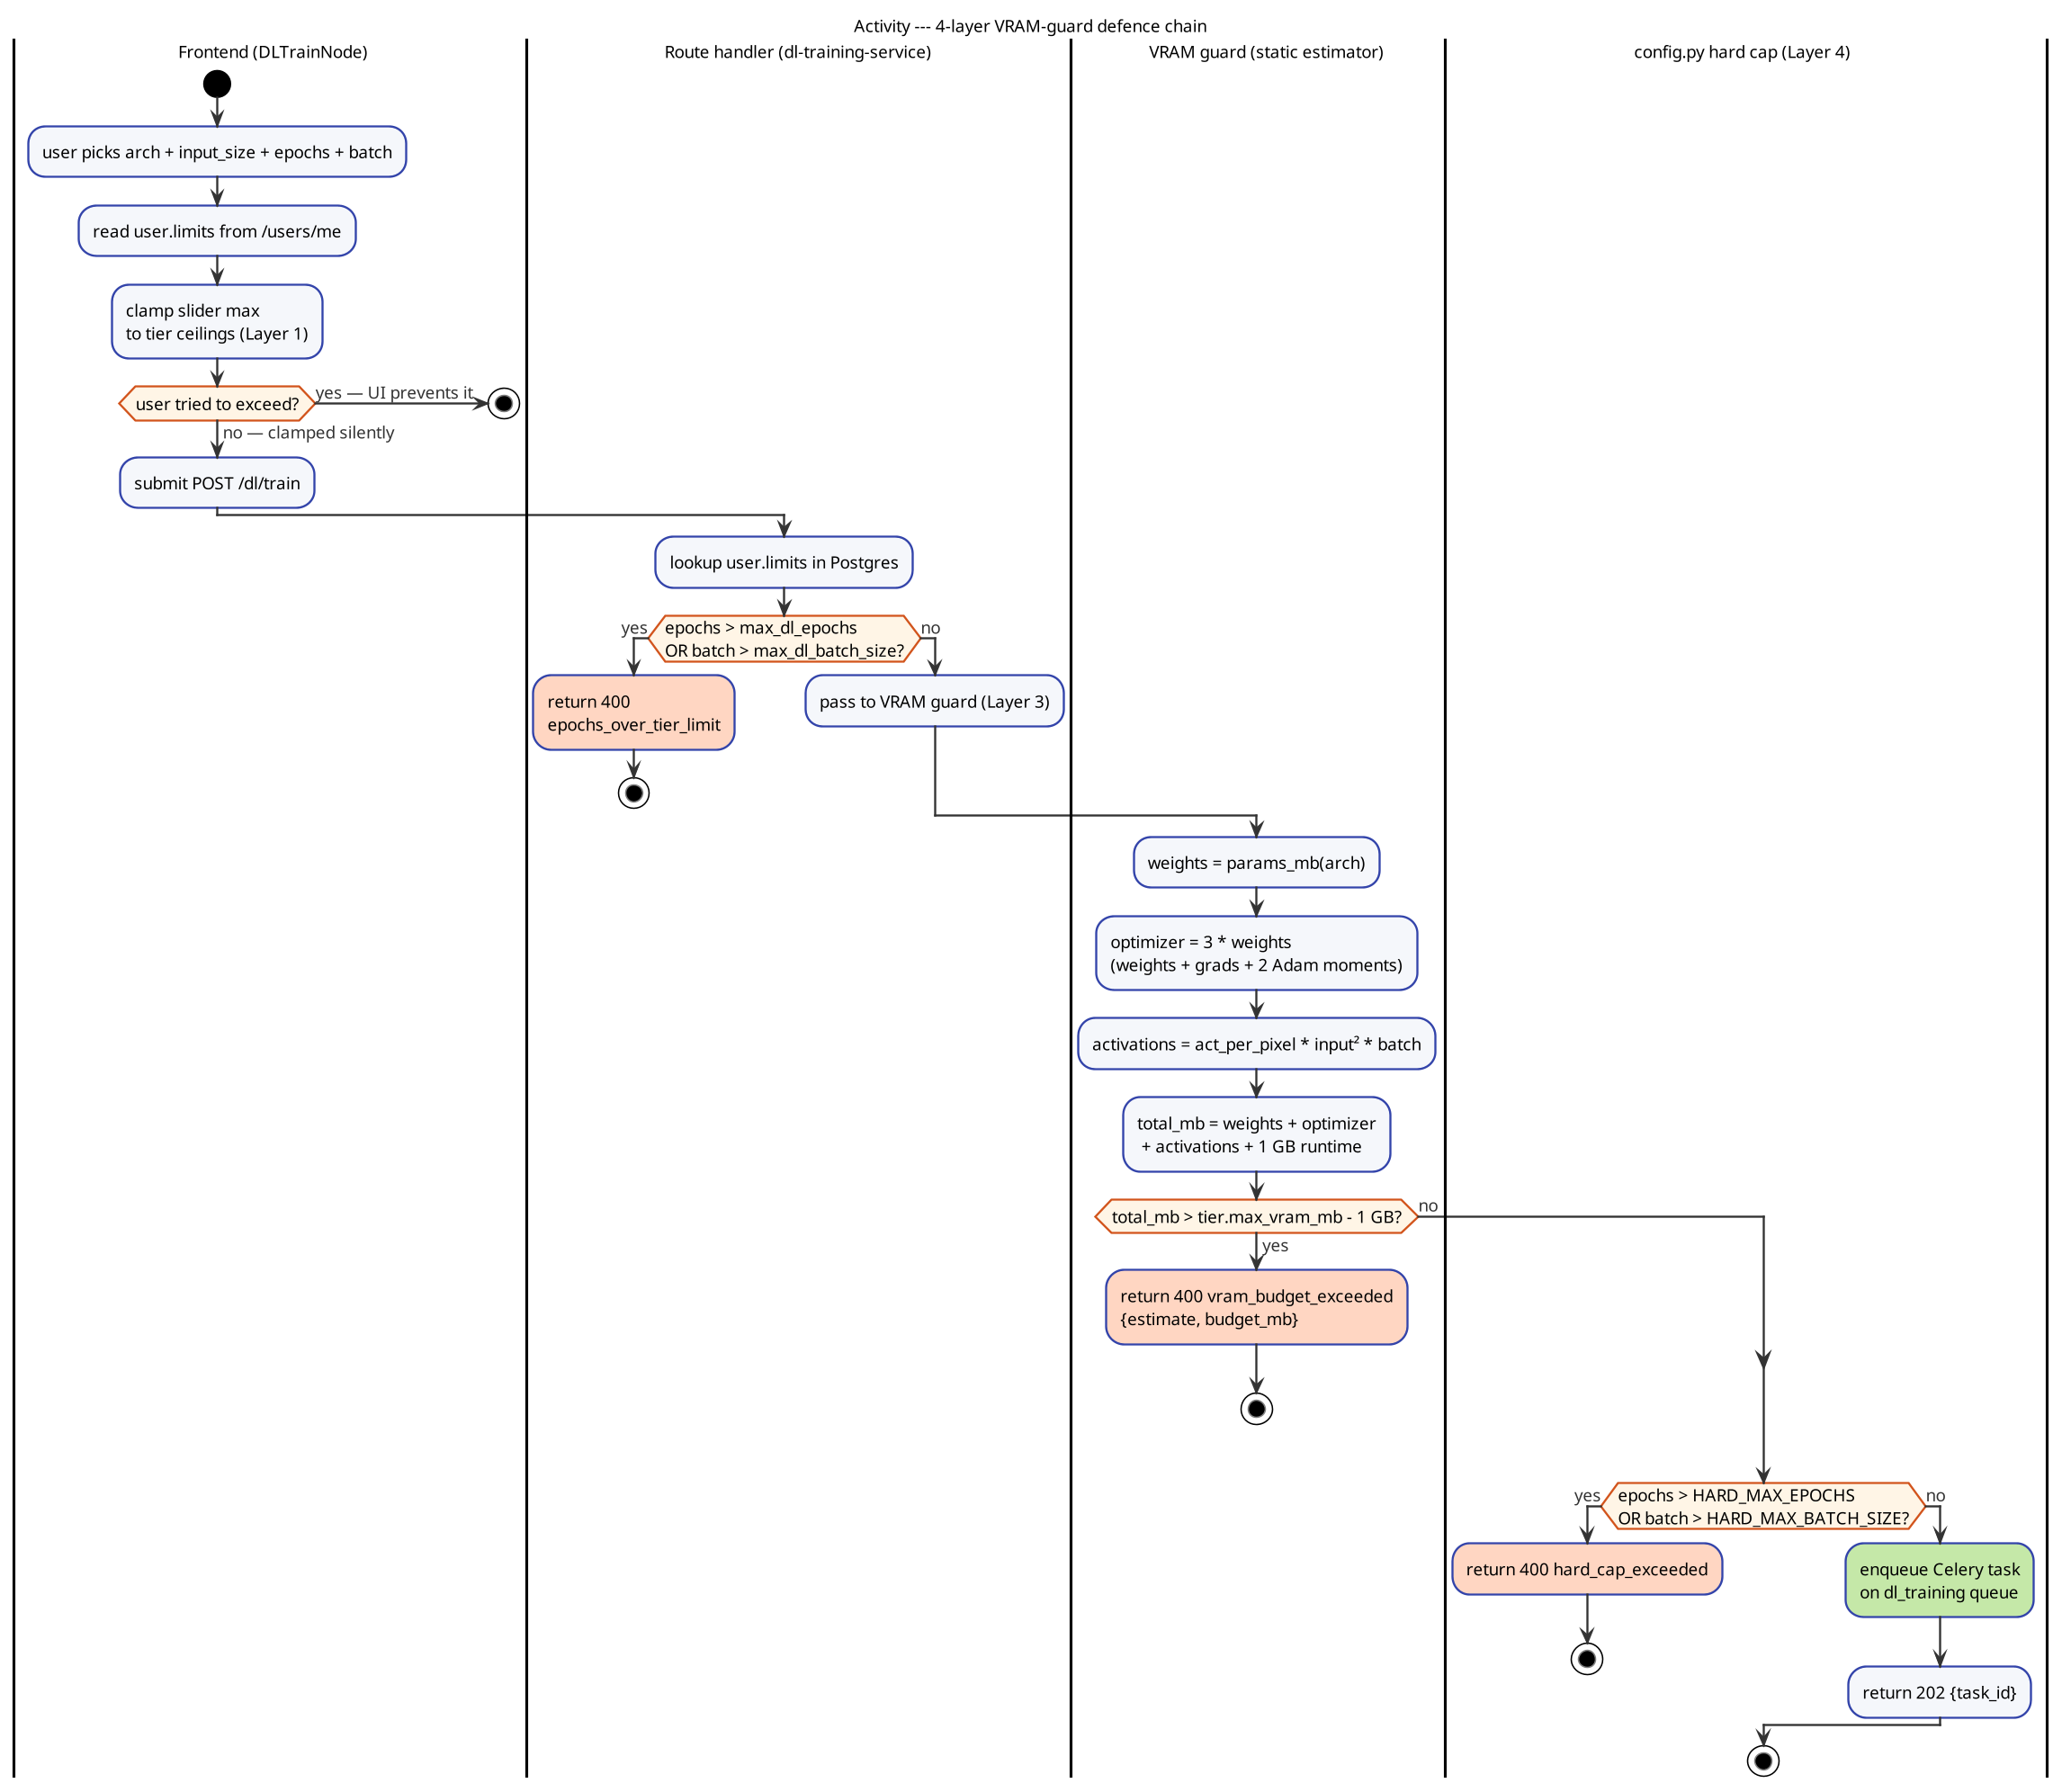
\includegraphics[width=0.85\textwidth, keepaspectratio]{diagrams/ch7_fig_activity_vram_guard}
  \caption{Activity diagram --- the four-layer VRAM-guard defence chain.}
  \label{fig:ch7_fig_activity_vram_guard}
\end{figure}

\subsection{Frontend integration}

% [FIGURE NEEDED: Pipeline editor screenshot in deep-learning mode --- Image Dataset, CNN Arch, DL Train nodes wired together]
% \begin{figure}[H]
%   \centering
%   \includegraphics[width=0.95\textwidth]{figures/placeholder_ch7_fig4}
%   \caption{Pipeline editor in deep-learning mode.}
%   \label{fig:ch7_fig4}
% \end{figure}

The canvas gained a third toggle button (``Deep Learning''), three
new node components (\texttt{ImageDatasetNode},
\texttt{CNNArchNode}, \texttt{DLTrainNode}), and a fourth preset
(\texttt{dlStarter}). The three-family lock logic was extended to
lock all three families against each other once any node of a given
family lands on the canvas.

The \texttt{ImageDatasetNode} body shows class chips, total-image
count, and a deterministically seeded thumbnail strip (three images
per class, pulled from \texttt{/datasets/<id>/image-preview} as
base64-encoded JPEGs). The \texttt{CNNArchNode} surfaces a
\texttt{pretrained} toggle that disables itself when the chosen
architecture has no canonical ImageNet checkpoint --- the user sees
\textit{why} the option is unavailable rather than having a control
silently disappear, which is the small UX detail that decides
whether people trust the interface.

% [FIGURE NEEDED: Close-up of the ImageDatasetNode --- class chips, image count, thumbnail strip]
% \begin{figure}[H]
%   \centering
%   \includegraphics[width=0.75\textwidth]{figures/placeholder_ch7_fig5}
%   \caption{ImageDatasetNode --- class chips, image count, thumbnail strip.}
%   \label{fig:ch7_fig5}
% \end{figure}

\subsection{Live progress and inference}

The training Celery task emits a \texttt{training\_epoch} socket
event per epoch with \texttt{\{epoch, train\_loss, val\_loss,
val\_acc\}}. The \texttt{LiveTrainingChart} component fans that
single event into three Plotly series sharing the same epoch-indexed
X-axis.

When training completes, a \texttt{DLPredictPanel} component renders
inline immediately under the success alert. The user drops an image,
the panel POSTs it to \texttt{/dl/predict/<version\_id>}, and the
top-five softmax probabilities render as ranked horizontal bars.

% [FIGURE NEEDED: DLPredictPanel screenshot --- dropped image preview, top-five softmax probabilities as ranked bars]
% \begin{figure}[H]
%   \centering
%   \includegraphics[width=0.85\textwidth]{figures/placeholder_ch7_fig6}
%   \caption{Inline DL prediction panel --- top-five softmax probabilities.}
%   \label{fig:ch7_fig6}
% \end{figure}

\subsection{Demo path end-to-end}

For the live demo, the path is:

\begin{enumerate}
    \item \texttt{python scripts/seed\_demo\_image\_dataset.py
        /tmp/demo.zip} --- generates a 30-image, 3-class synthetic
        dataset (red circles, green squares, blue triangles).
    \item Upload the zip from the Data page.
    \item Drop the \texttt{dlStarter} preset onto a fresh pipeline.
    \item Click Run. Roughly 30 seconds later, the predict panel
        renders.
    \item Drop an image --- one of the synthetic ones, or a real
        one from a phone --- and inference returns in roughly
        $5$\,ms on CPU.
\end{enumerate}

The reference DL validation run uses tiny\_resnet at $64$\,px,
batch~32, five epochs against the synthetic dataset. Terminal
validation accuracy lands at $100\%$ in roughly $30$ seconds on a
1660 Super --- a number that is honest about the dataset's
simplicity (three visually distinct classes) but proves the full
pipeline.

A separate \texttt{scripts/dl\_smoke.sh} script exercises the entire
chain non-interactively: gateway reachability, GPU visibility, the
oversize-refusal path, the demo run, and the polling loop. The
script has caught regressions in seemingly unrelated services more
than once.

\section{Unit Tests}

The \texttt{dl-training-service} ships 22 unit tests:

\begin{itemize}
    \item Architecture forward-pass shapes --- one test per
        architecture on a known input tensor.
    \item VRAM-guard envelope --- parametrised over every
        documented \texttt{(arch, input\_size, batch\_size)}
        triple, asserts the estimate sits under the
        6\,GB-minus-1\,GB budget.
    \item Oversize refusal --- a request with an obviously oversized
        batch is rejected by the route before training starts.
    \item End-to-end \texttt{build $\to$ save $\to$ predict} on
        a tiny LeNet against a 12-image fixture dataset, against
        a real torch instance (CPU on CI).
    \item Tier-ceiling enforcement --- a free-tier token posting
        20 epochs is rejected with the documented error code.
\end{itemize}

\section*{Conclusion}

Sprint~4 was the riskiest sprint of the project. Bolting an entirely
new workload onto a platform that had calmed down into three sprints
of mostly-tabular and RAG work could have destabilised the whole
thing. It did not, mostly because the conventions established in
earlier sprints --- the shared-volume pattern, the Celery-per-service
split, the gateway header injection --- absorbed the new service
without bending.

% ═════════════════════════════════════════════════════════════════════════════
\chapter{Sprint 5: Multi-tenancy, Project ACL, and Real-Time Collaboration}
% ═════════════════════════════════════════════════════════════════════════════

\section*{Introduction}

Up to this point the platform had been a single-user experience.
The company-tier story needed something else: multiple people on the
same pipeline at the same time, with sensible access controls and
enough real-time feedback that they would not accidentally undo each
other's work.

\section{Sprint Backlog}

\begin{table}[H]
\centering
\caption{Sprint~5 backlog --- multi-tenancy and collaboration.}
\label{tab:sprint5_backlog}
\begin{tabular}{@{}p{0.05\linewidth} L{0.55\linewidth} p{0.1\linewidth} p{0.18\linewidth}@{}}
\toprule
\textbf{ID} & \textbf{User Story / Task} & \textbf{Priority} & \textbf{Estimation (d)} \\
\midrule
US-37 & Per-pipeline access control with five distinct roles. & High & 1.5 \\
US-38 & Server-side and client-side role enforcement. & High & 1 \\
US-39 & Real-time canvas presence (cursors and node highlights). & High & 2 \\
US-40 & Threaded chat per pipeline. & Medium & 1.5 \\
US-41 & One-click Google Meet links via Google OAuth. & Medium & 1 \\
US-42 & Per-pipeline notification fan-out. & Medium & 0.5 \\
\bottomrule
\end{tabular}
\end{table}

\section{Concepts fondamentaux}

\textbf{SocketIO rooms.} A room is a server-side label that groups
client connections; emitting to a room fans the message out to every
connection joined to that label. The collaboration layer joins each
client to the room \texttt{pipeline\_<id>} the moment the pipeline
opens, and unjoins on unmount.

\textbf{Throttling for real-time presence.} Cursor moves can fire at
60\,Hz; broadcasting every event saturates the message bus and the
clients without adding signal. The frontend throttles to one event
per 50\,ms, which is below the human perception threshold for
cursor lag and an order of magnitude lighter on the network.

\textbf{Authoritative role resolution at the gateway.} The five
roles (Owner, Project Manager, Data Scientist, Analyst, Viewer) are
resolved at the gateway and stamped onto \texttt{X-Project-Role}
just like \texttt{X-User-Id}. Downstream services trust the header
without re-checking, which keeps the zero-trust boundary
single-layered.

\section{Design}

\begin{figure}[H]
  \centering
  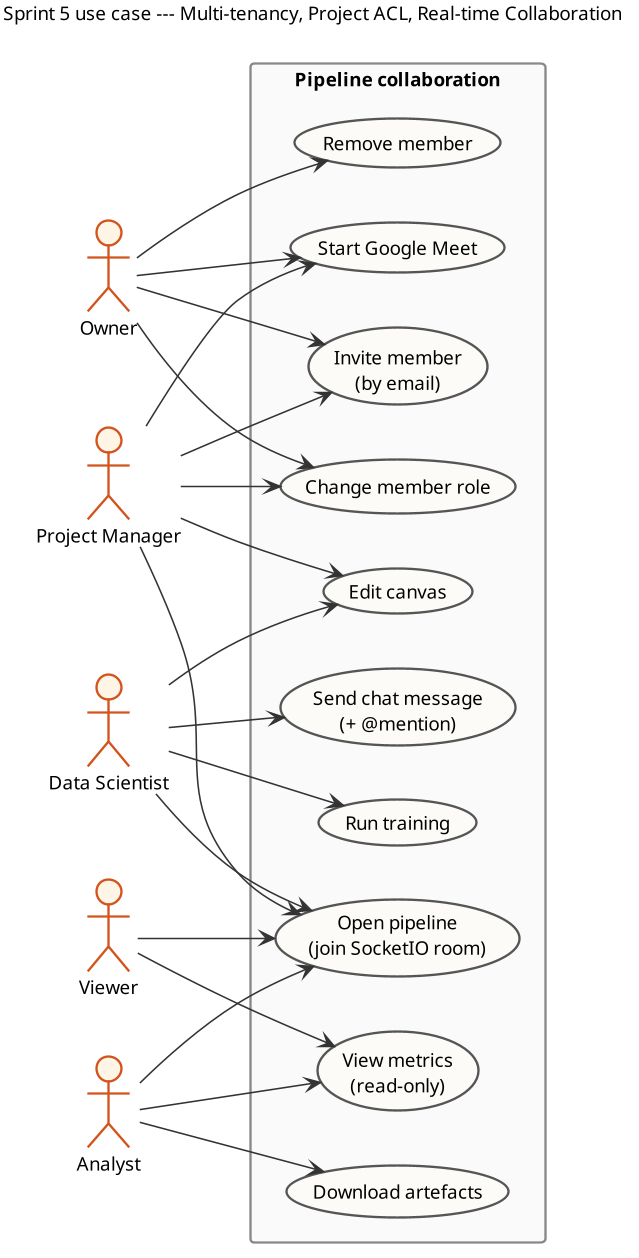
\includegraphics[height=0.9\textheight, keepaspectratio]{diagrams/ch8_fig1}
  \caption{Use case diagram --- collaboration roles and actions.}
  \label{fig:ch8_fig1}
\end{figure}

\begin{figure}[H]
  \centering
  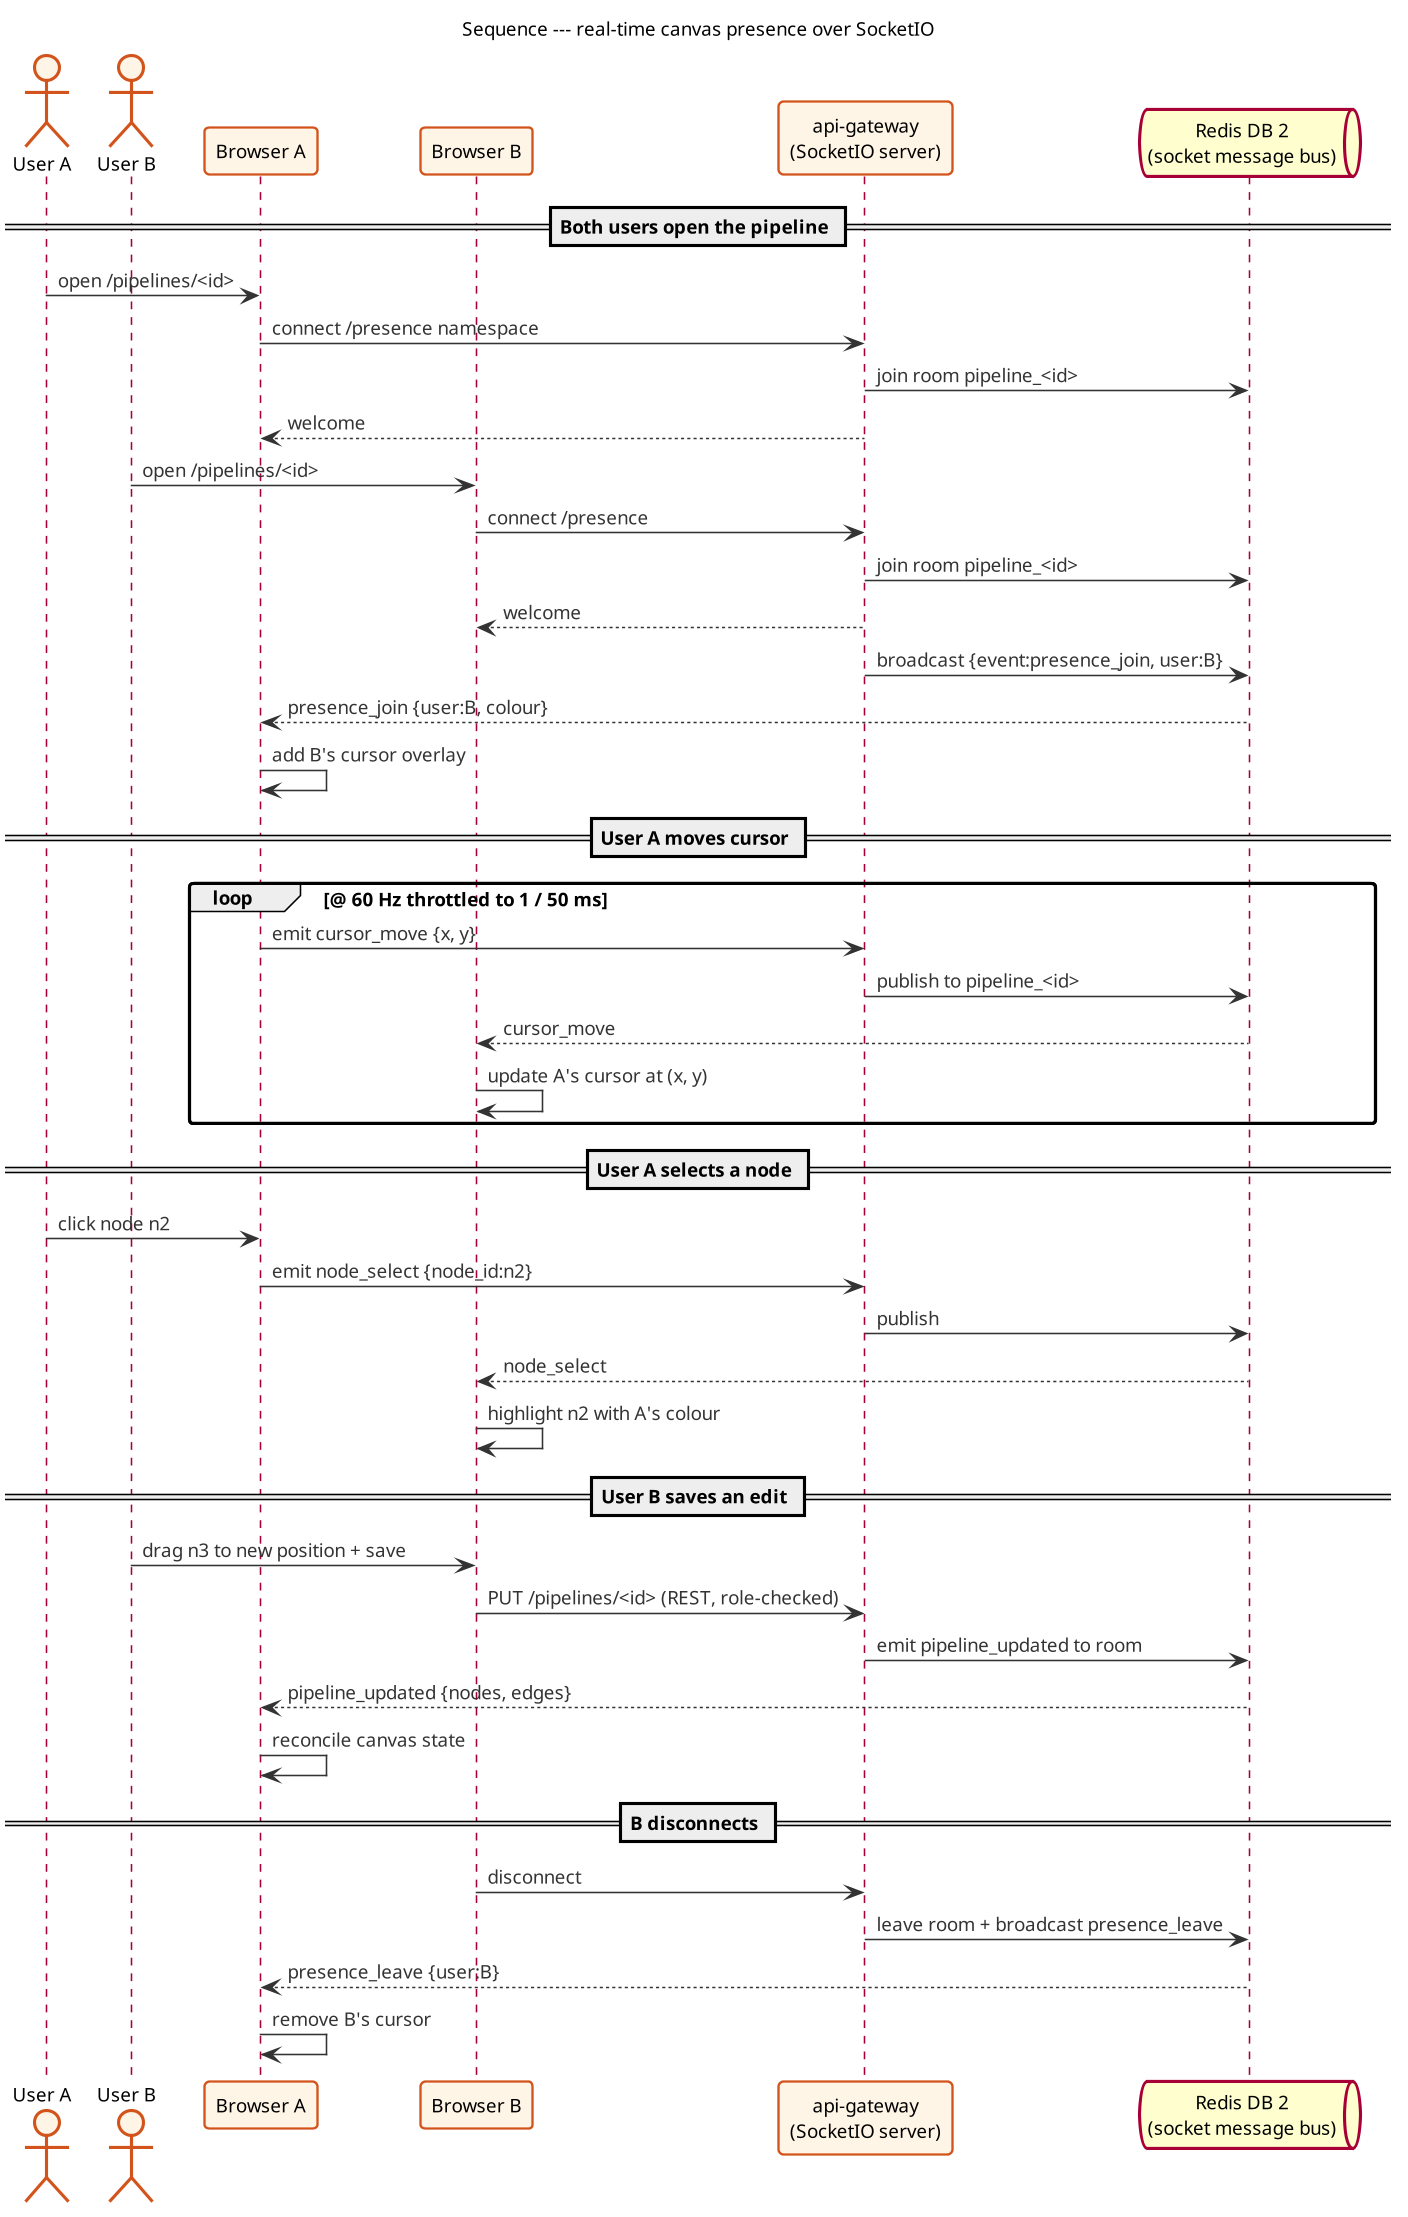
\includegraphics[width=0.85\textwidth, keepaspectratio]{diagrams/ch8_fig2}
  \caption{Sequence diagram --- cursor and node-selection events over SocketIO.}
  \label{fig:ch8_fig2}
\end{figure}

\begin{figure}[H]
  \centering
  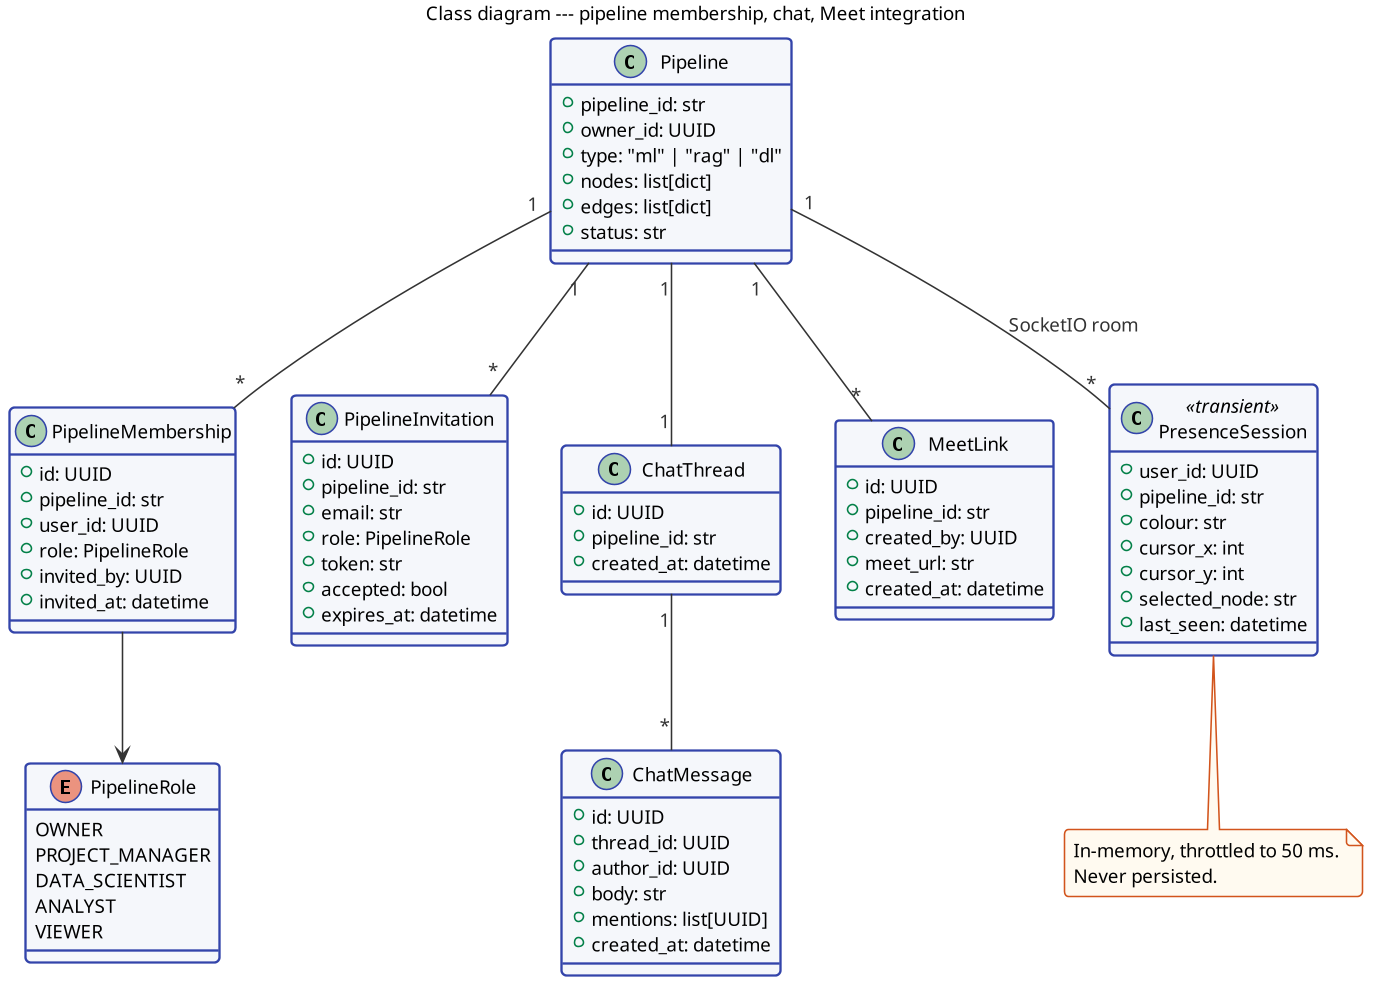
\includegraphics[width=0.85\textwidth, keepaspectratio]{diagrams/ch8_fig3}
  \caption{Class diagram --- pipeline membership, chat threads, Meet integration.}
  \label{fig:ch8_fig3}
\end{figure}

\begin{figure}[H]
  \centering
  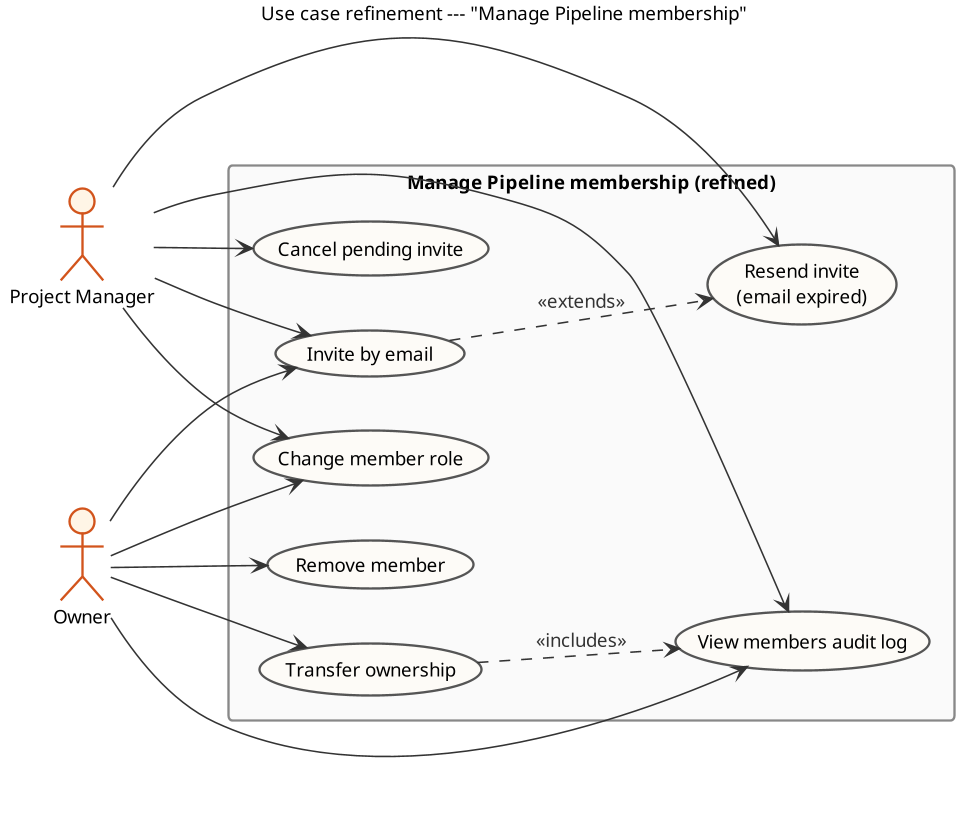
\includegraphics[width=0.85\textwidth, keepaspectratio]{diagrams/ch8_fig_uc_refine_pipeline}
  \caption{Use-case refinement --- ``Manage Pipeline membership'' broken into sub-cases.}
  \label{fig:ch8_fig_uc_refine_pipeline}
\end{figure}

\subsection{The role hierarchy}

\begin{itemize}
    \item \textbf{Owner} --- the user who created the pipeline.
        Cannot be removed.
    \item \textbf{Project Manager} --- can invite, can edit, cannot
        remove the owner.
    \item \textbf{Data Scientist} --- can edit nodes, can run
        training, cannot manage members.
    \item \textbf{Analyst} --- can view metrics and download
        artefacts, cannot run training.
    \item \textbf{Viewer} --- read-only.
\end{itemize}

The role is enforced both server-side and client-side. The gateway
resolves the user's role for the project on every
\texttt{/pipelines/*} request and stamps \texttt{X-Project-Role};
the frontend disables UI affordances based on the same role.
Server-side enforcement is authoritative; the client-side disable is
UX, not security. Mixing those up is one of the easier mistakes in
this area.

% [FIGURE NEEDED: Manage Access dialog screenshot --- invite by email, change role, remove]
% \begin{figure}[H]
%   \centering
%   \includegraphics[width=0.75\textwidth]{figures/placeholder_ch8_fig4}
%   \caption{Manage Access dialog --- invite, role change, remove.}
%   \label{fig:ch8_fig4}
% \end{figure}

\section{Implementation}

\subsection{Real-time presence}

When a user opens a pipeline, the gateway joins them to the
\texttt{pipeline\_<id>} SocketIO room. Cursor positions and node
selections are emitted as throttled (50\,ms) events. The frontend
maintains a per-user coloured cursor overlay on the canvas. Watching
another user's cursor move across your screen is a small touch that
makes the platform feel inhabited in a way that chat alone never
quite does.

% [FIGURE NEEDED: Side-by-side screenshot --- two browser windows on the same pipeline, each showing the other's cursor and node highlight]
% \begin{figure}[H]
%   \centering
%   \includegraphics[width=0.95\textwidth]{figures/placeholder_ch8_fig5}
%   \caption{Real-time presence --- two users editing the same pipeline.}
%   \label{fig:ch8_fig5}
% \end{figure}

\subsection{Pipeline chat and Google Meet}

Each pipeline gets its own threaded chat, persisted to Postgres.
An ``@'' mention fires a notification (which the Sprint~6 bell
surfaces). The Google Meet integration relies on Google's OAuth flow
--- not for data-sharing reasons, but because a Meet link generated
server-side without OAuth is not tied to the inviting user's
calendar, which makes the link useless for the actual workflow.

\subsection{Why the gateway resolves the role}

The role-resolution lookup happens inside the gateway rather than in
each downstream service. Two reasons.

First, the gateway already maintains the request-scoped user
identity. Adding role resolution here keeps the zero-trust pattern
intact --- downstream services trust the stamped
\texttt{X-Project-Role} the same way they trust
\texttt{X-User-Id}.

Second, it centralises the cache. A short-lived Redis-backed cache
on \texttt{(user\_id, pipeline\_id) $\to$ role} cuts the
auth-service lookup count to a small fraction of the request count,
without spreading caching logic across four services.

\section{Unit Tests}

\begin{itemize}
    \item Role-matrix table-test: for each (role, action) pair, the
        expected permit/deny outcome.
    \item Role demotion mid-session: a Project Manager has their
        role downgraded to Viewer while connected; the next
        canvas-edit event is rejected.
    \item Owner immutability: an attempt to remove the owner
        returns the documented error code.
    \item SocketIO presence: two test clients join the same
        pipeline room and assert that each sees the other's
        cursor events.
\end{itemize}

\section*{Conclusion}

The collaboration layer turned the platform from a personal tool
into something a team could share. The interesting part of this
sprint was how little of the existing architecture had to change to
support it --- the gateway already injected user identity, the
SocketIO bus was already in place for live training, and the role
check fit naturally into the existing header convention.

% ═════════════════════════════════════════════════════════════════════════════
\chapter{Sprint 6: Dashboard, i18n, Accessibility, and Admin Console}
% ═════════════════════════════════════════════════════════════════════════════

\section*{Introduction}

Every project has the sprint where the punch list of small things
finally gets crossed off. This was that sprint. The dashboard, the
billing UI, internationalisation, the high-contrast theme, the
notification bell, the admin operations dashboard, user
impersonation, and undo/redo on the canvas --- each modest on its
own, but together they moved the platform from ``demonstrably
works'' to ``demonstrably operable''.

\section{Sprint Backlog}

\begin{table}[H]
\centering
\caption{Sprint~6 backlog --- operability and polish.}
\label{tab:sprint6_backlog}
\begin{tabular}{@{}p{0.05\linewidth} L{0.55\linewidth} p{0.1\linewidth} p{0.18\linewidth}@{}}
\toprule
\textbf{ID} & \textbf{User Story / Task} & \textbf{Priority} & \textbf{Estimation (d)} \\
\midrule
US-43 & User-facing dashboard (datasets, pipelines, model versions). & High & 1.5 \\
US-44 & Billing UI (free / solo / company tier; Stripe checkout). & High & 2 \\
US-45 & Internationalisation (English + French, generated bindings). & High & 1 \\
US-46 & High-contrast theme + WCAG~AA audit. & Medium & 1 \\
US-47 & Persistent notification bell. & Medium & 1 \\
US-48 & Admin operations dashboard (5 panels). & High & 2 \\
US-49 & User impersonation with hard five-minute TTL. & High & 1 \\
US-50 & Undo / redo on the canvas with drag-coalescing. & Medium & 1 \\
\bottomrule
\end{tabular}
\end{table}

\section{Design}

\begin{figure}[H]
  \centering
  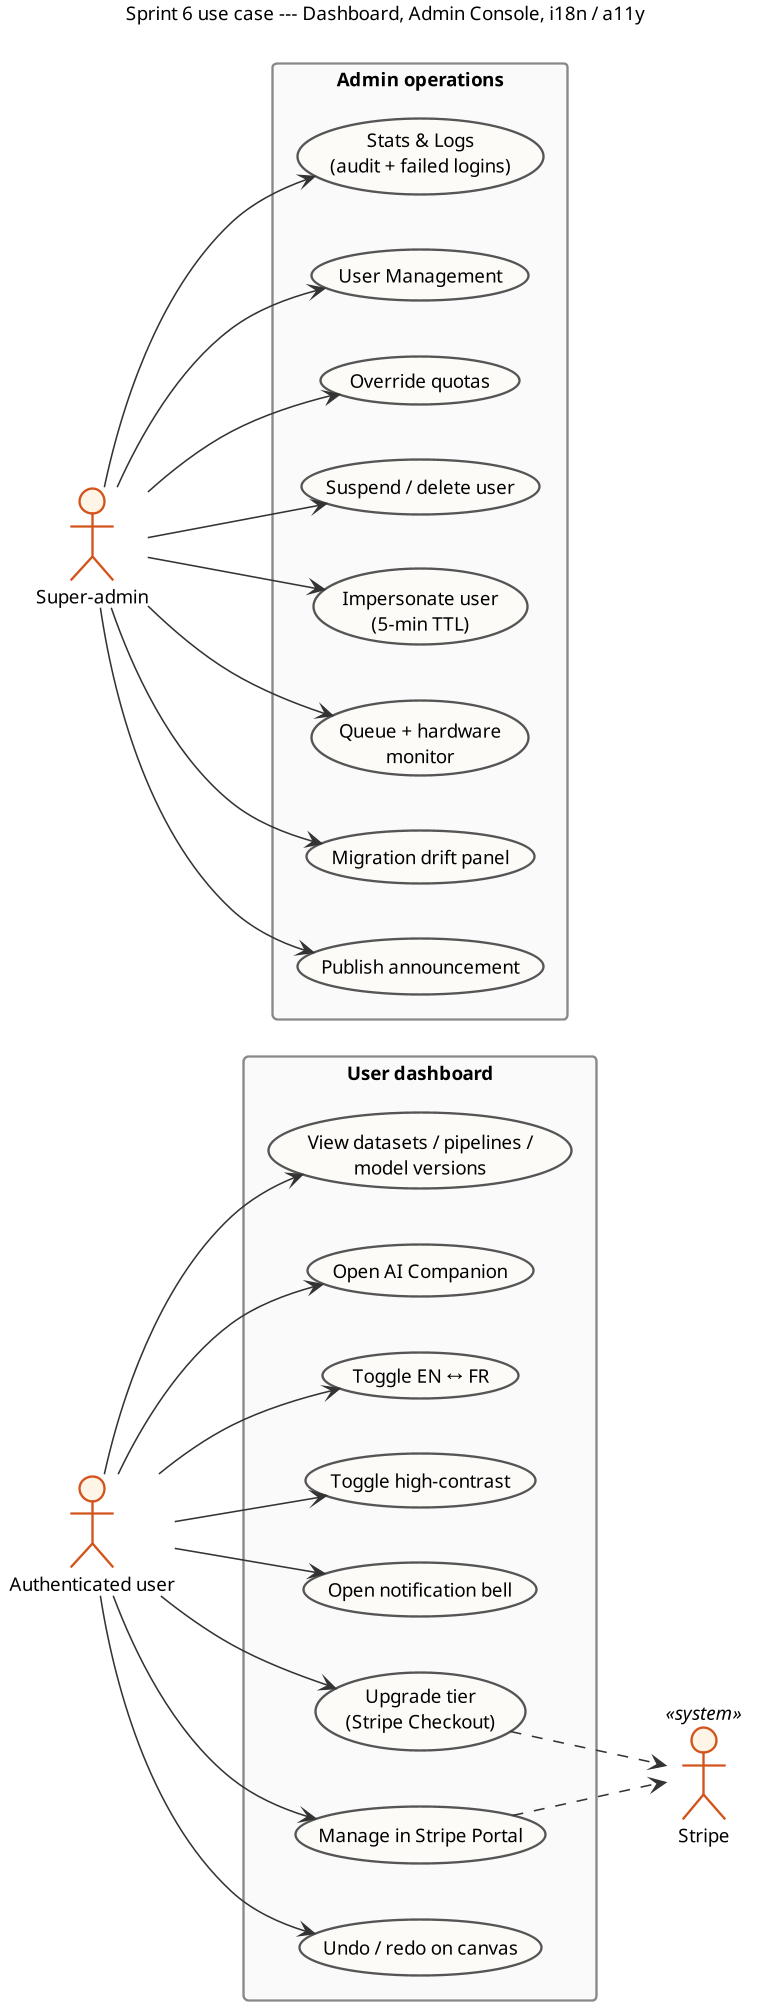
\includegraphics[height=0.9\textheight, keepaspectratio]{diagrams/ch9_fig1}
  \caption{Use case diagram --- dashboard plus admin operations.}
  \label{fig:ch9_fig1}
\end{figure}

\begin{figure}[H]
  \centering
  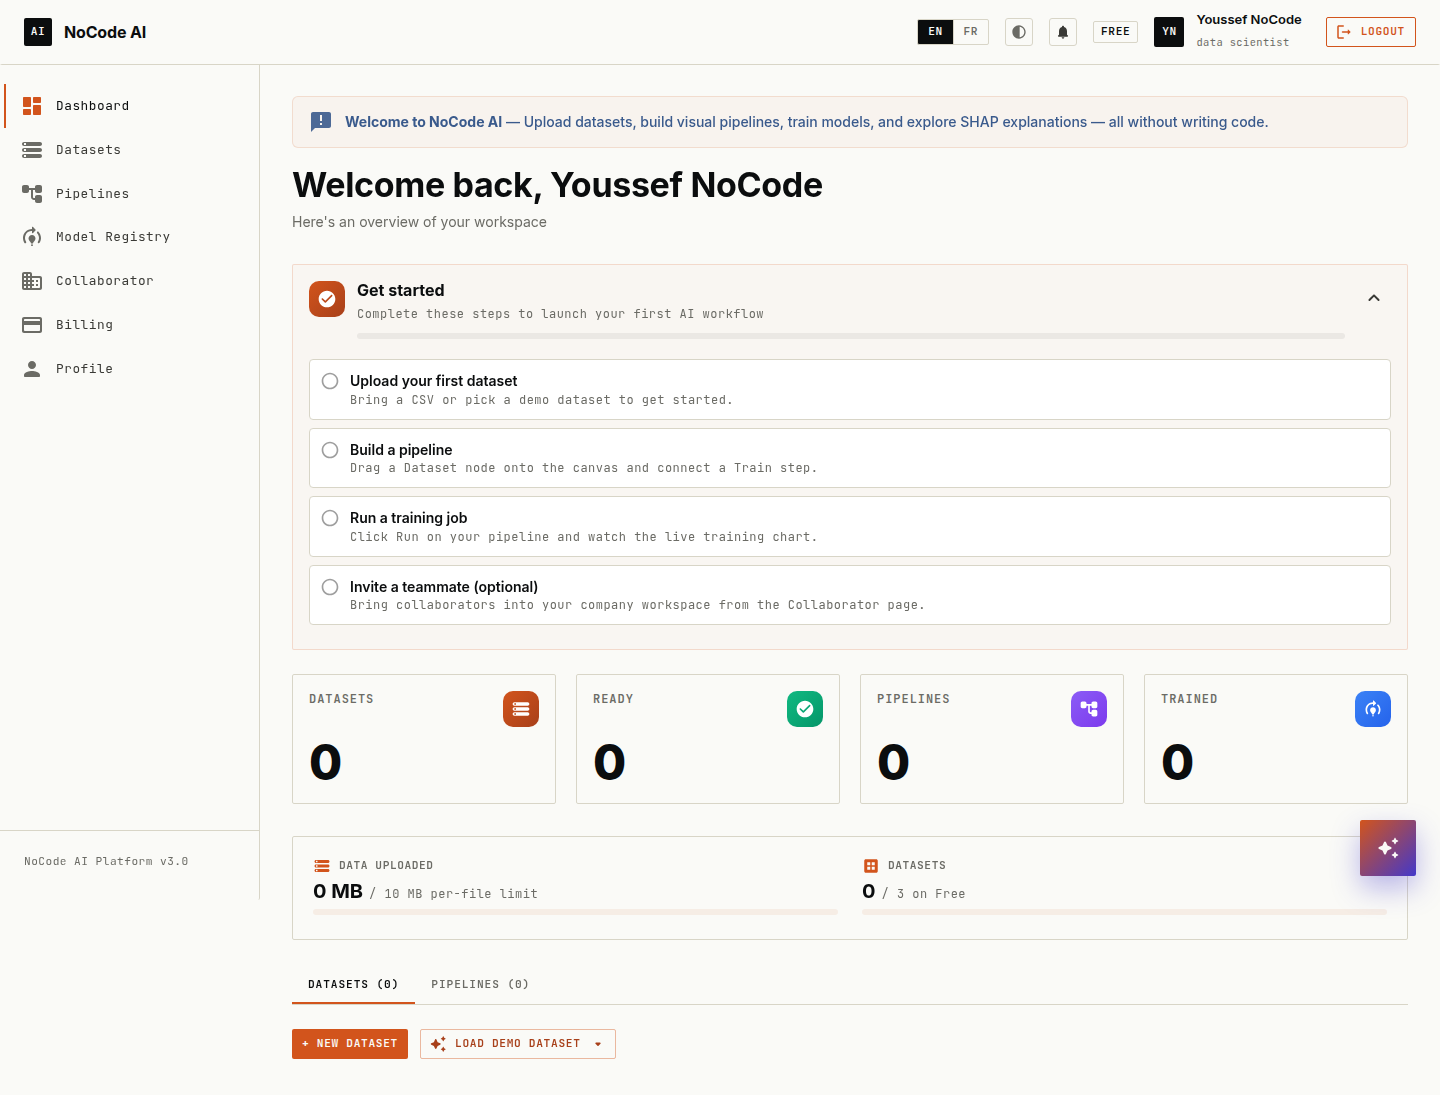
\includegraphics[width=0.85\textwidth, keepaspectratio]{diagrams/ch9_fig2}
  \caption{Wireframe --- user dashboard with datasets, pipelines, versions.}
  \label{fig:ch9_fig2}
\end{figure}

\begin{figure}[H]
  \centering
  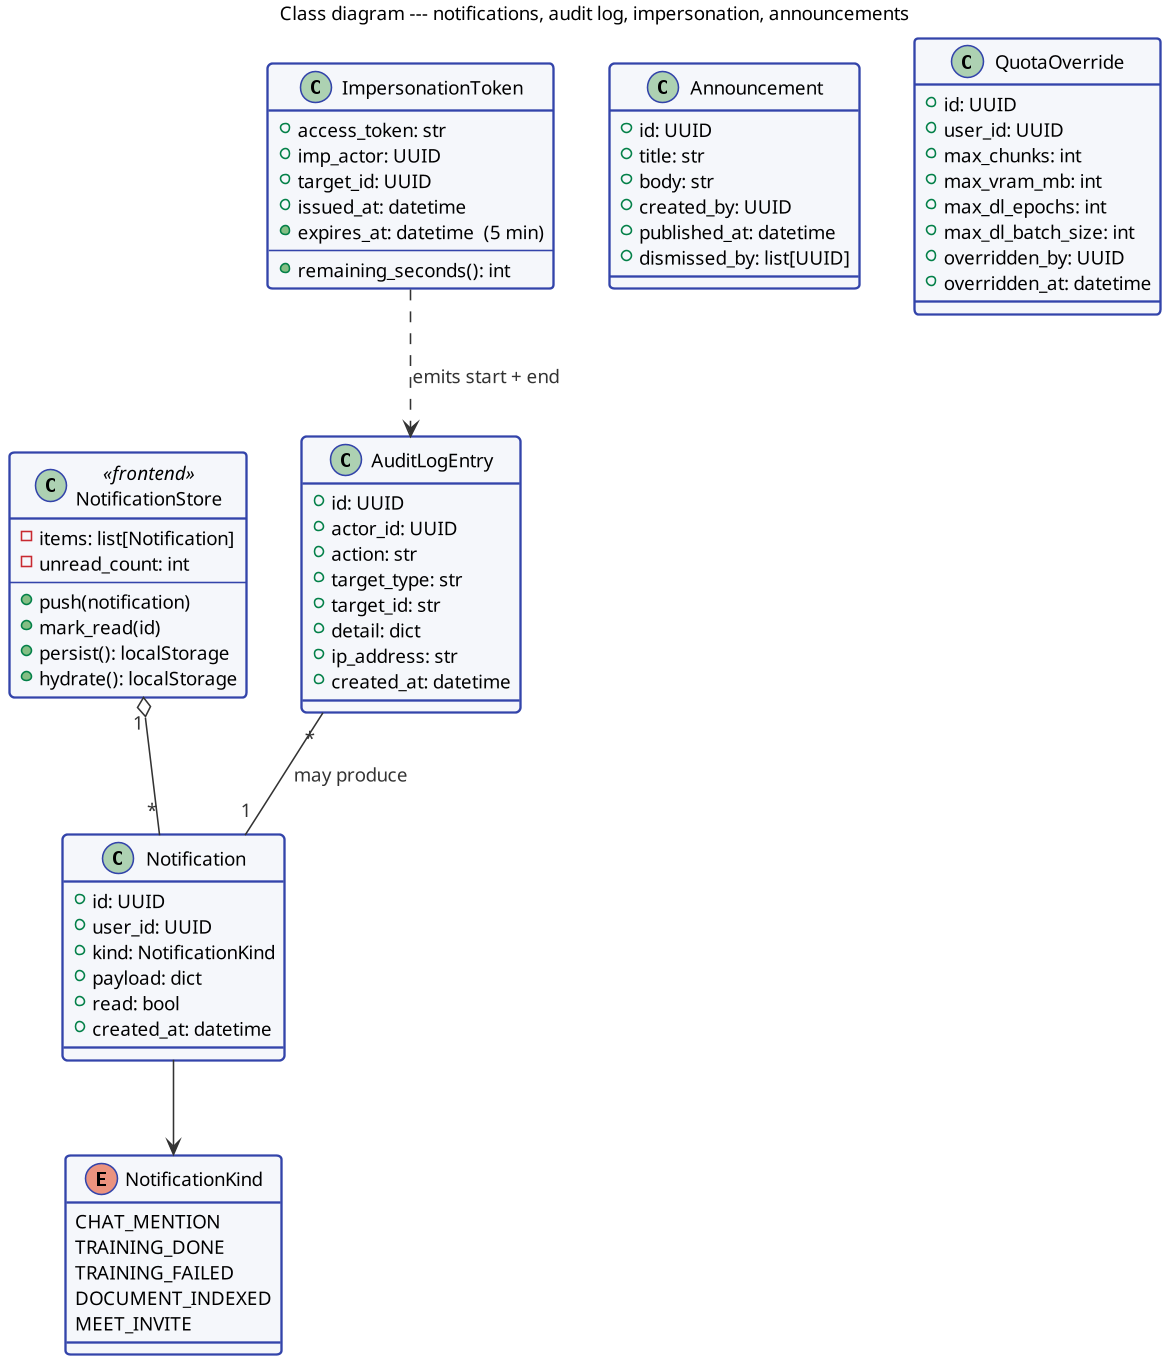
\includegraphics[width=0.85\textwidth, keepaspectratio]{diagrams/ch9_fig3}
  \caption{Class diagram --- notifications, audit log, impersonation token.}
  \label{fig:ch9_fig3}
\end{figure}

\begin{figure}[H]
  \centering
  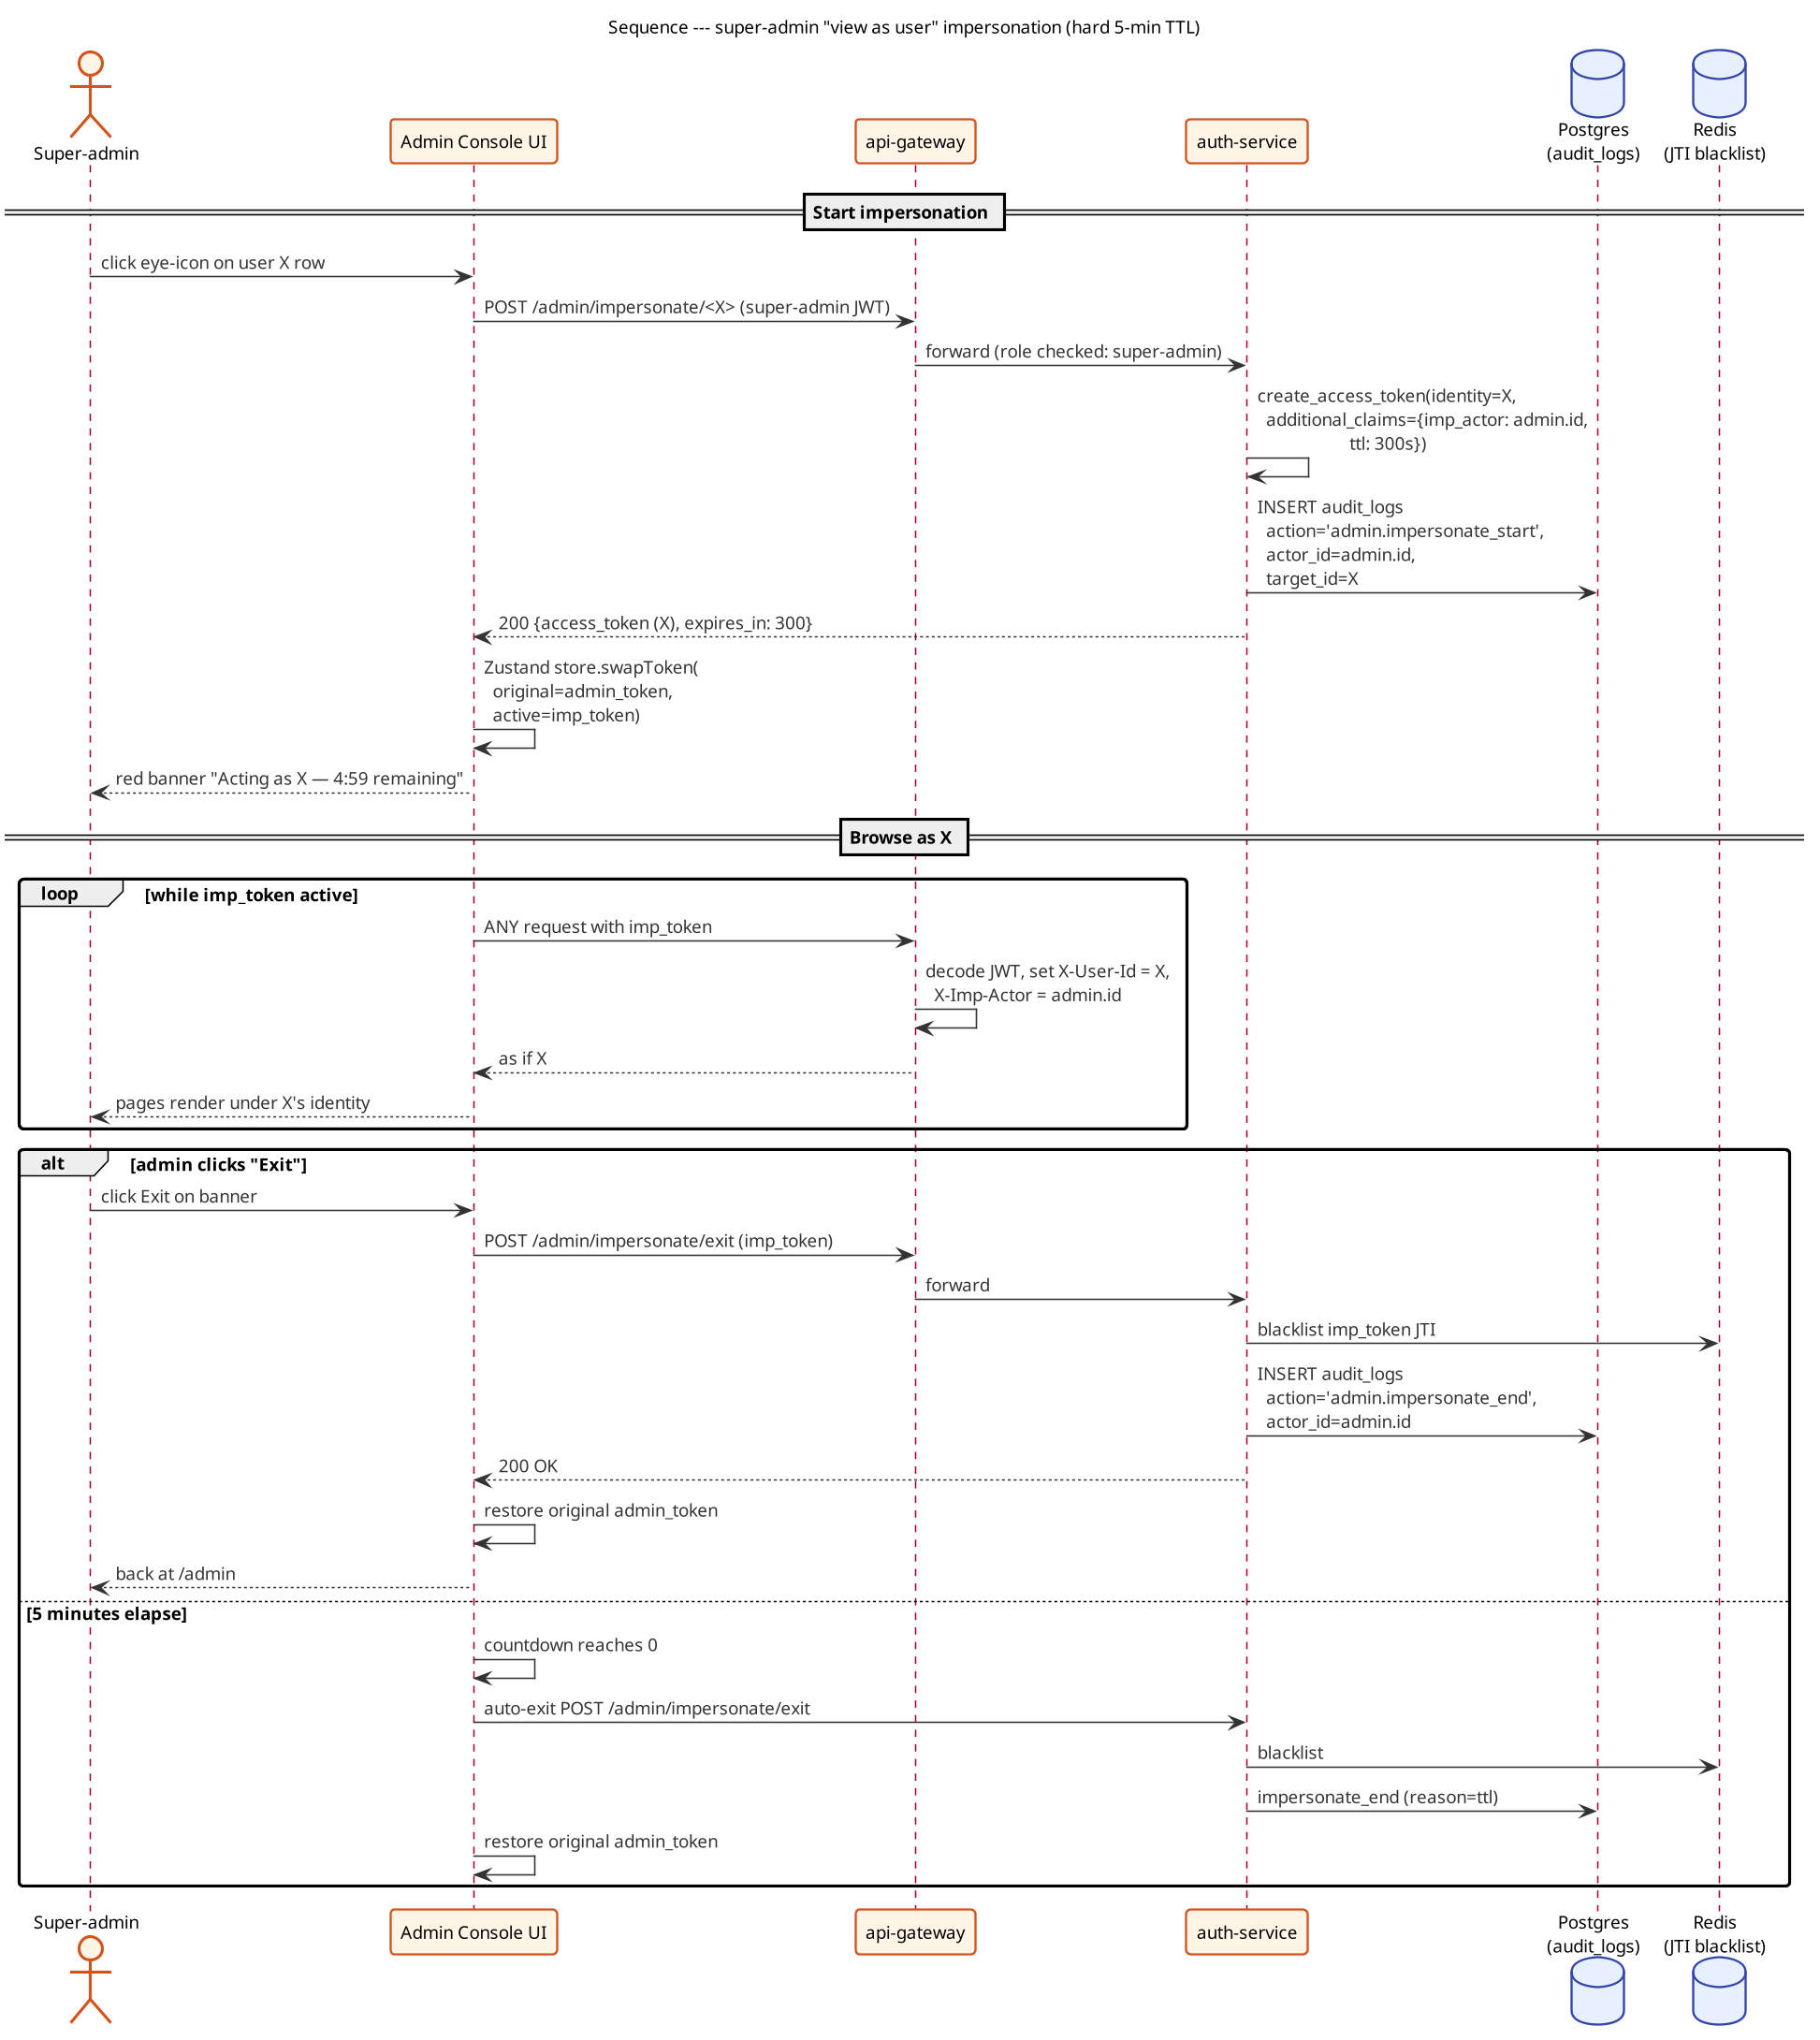
\includegraphics[width=0.85\textwidth, keepaspectratio]{diagrams/ch9_fig_seq_impersonate}
  \caption{Sequence diagram --- super-admin ``view as user'' impersonation with 5-minute TTL.}
  \label{fig:ch9_fig_seq_impersonate}
\end{figure}

\section{Implementation}

\subsection{The user dashboard and billing UI}

\begin{figure}[H]
  \centering
  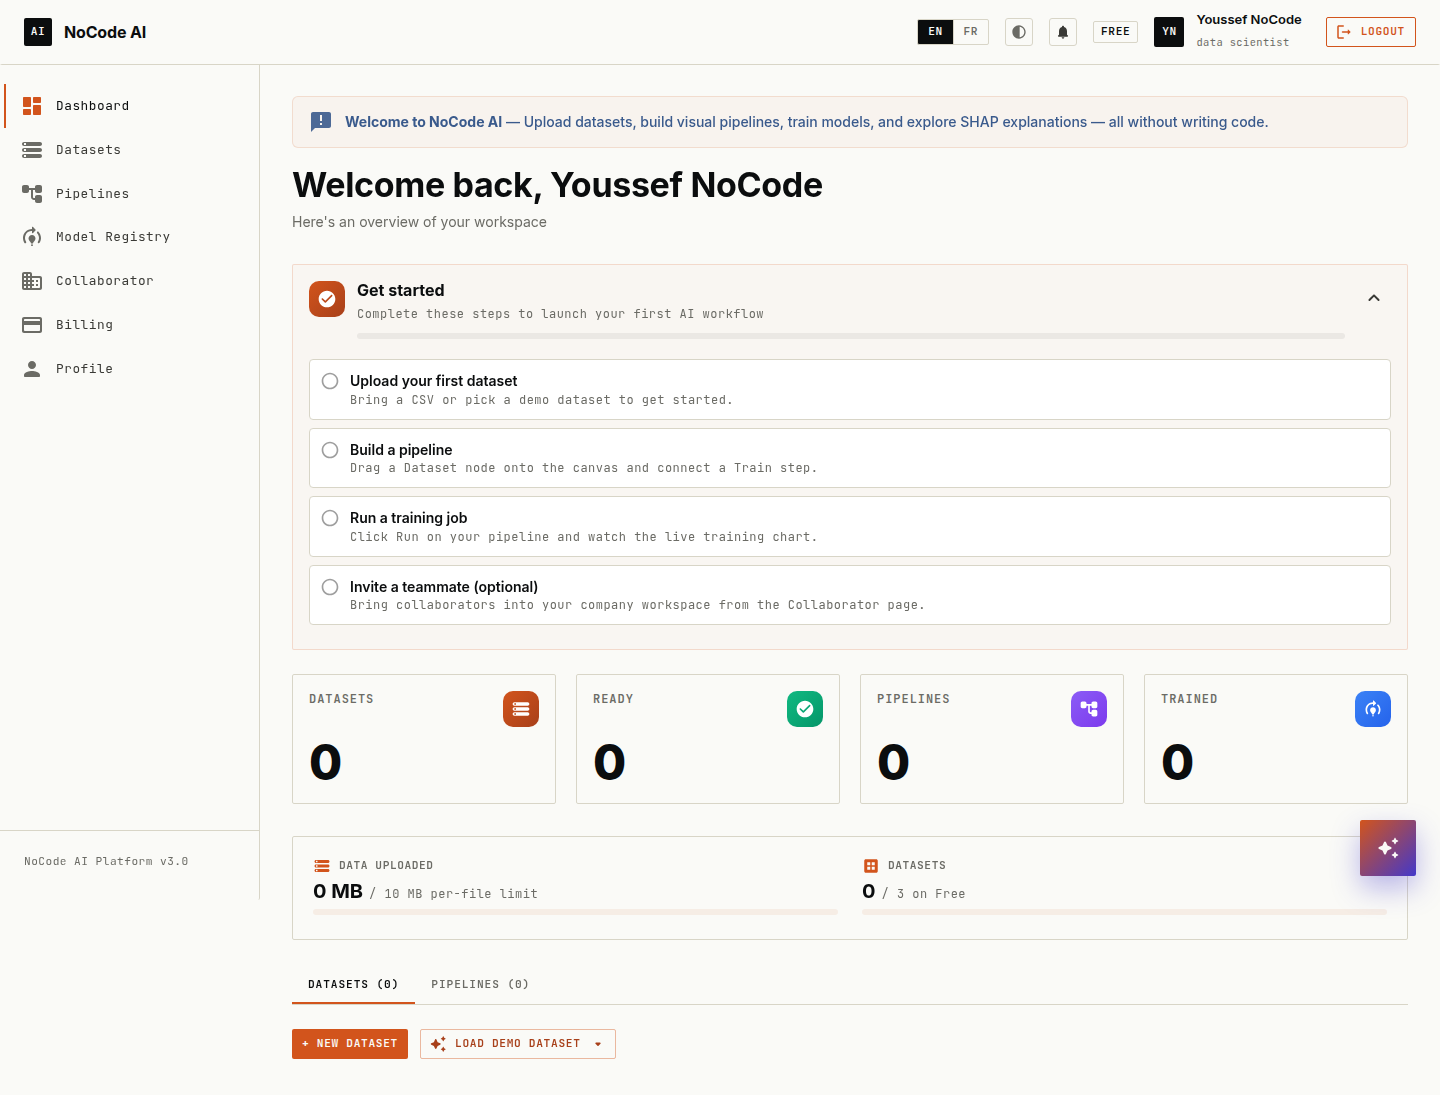
\includegraphics[width=0.85\textwidth, keepaspectratio]{diagrams/ch9_fig4}
  \caption{User dashboard --- datasets, pipelines, model versions, quota.}
  \label{fig:ch9_fig4}
\end{figure}

\begin{figure}[H]
  \centering
  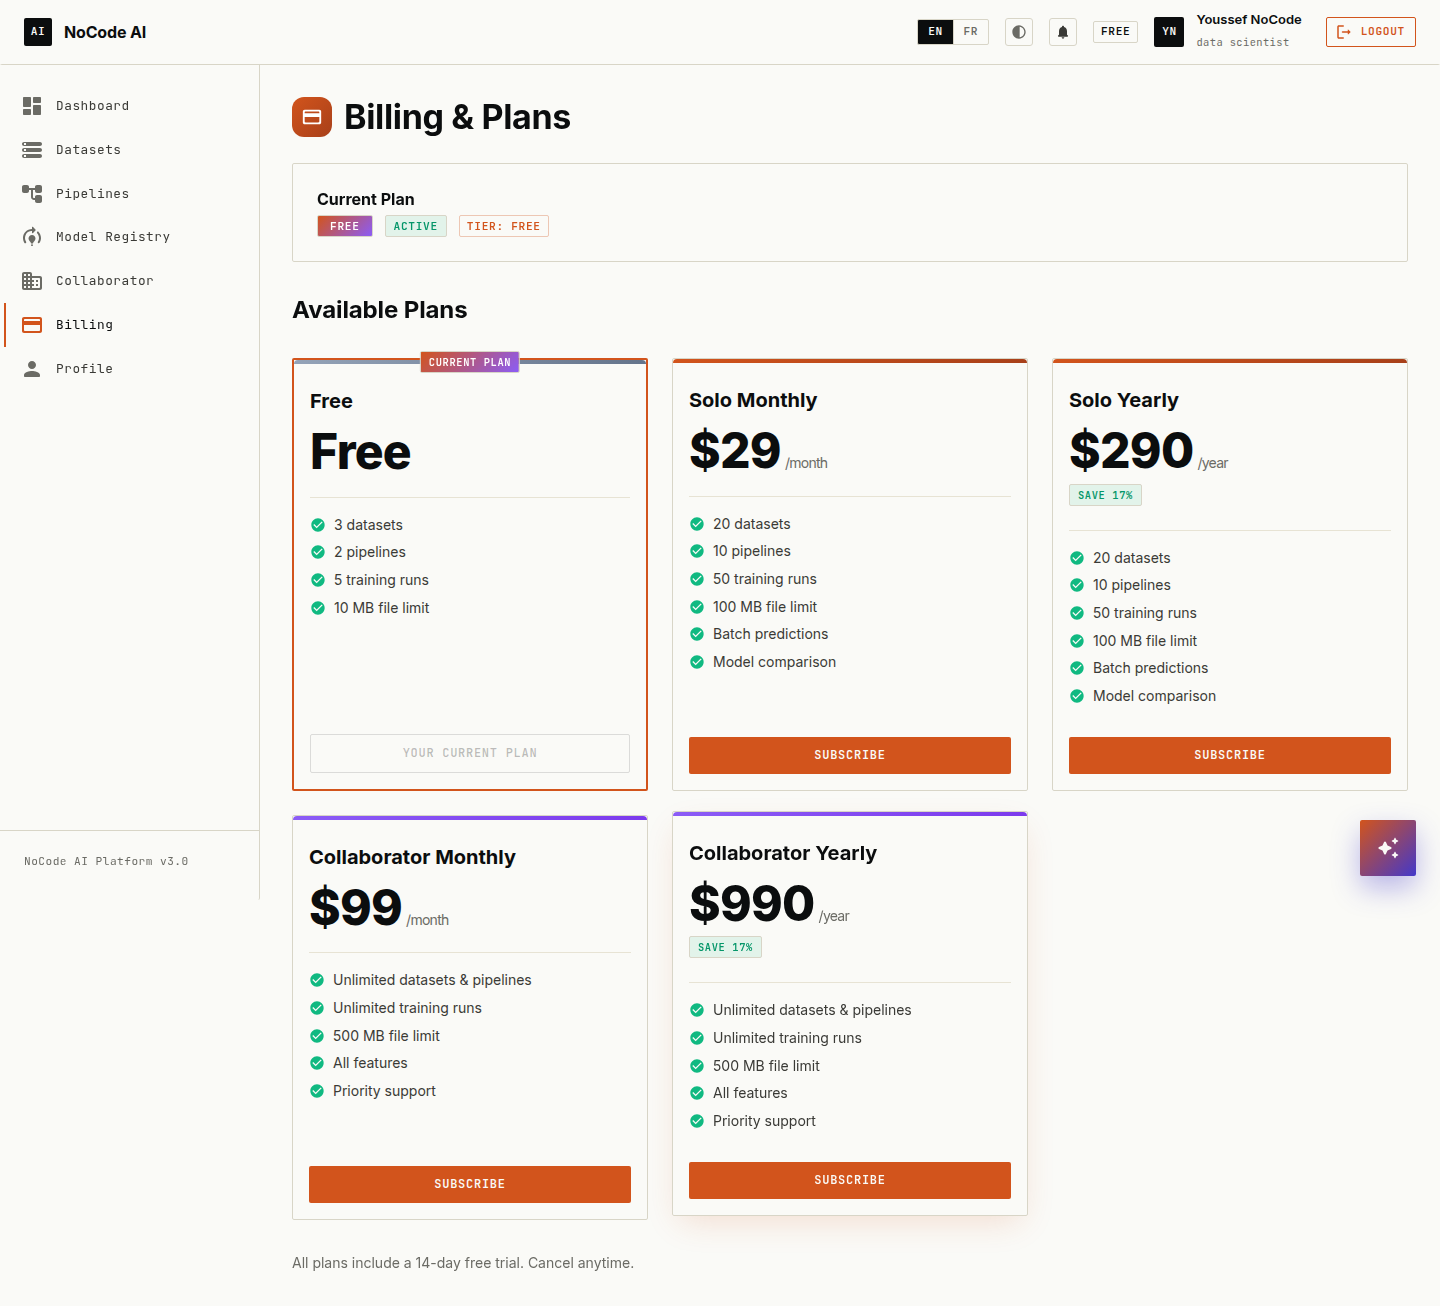
\includegraphics[width=0.85\textwidth, keepaspectratio]{diagrams/ch9_fig5}
  \caption{Billing page --- tier selection, Stripe checkout.}
  \label{fig:ch9_fig5}
\end{figure}

The dashboard is a single page with three tabs (Datasets, Pipelines,
Models), each backed by a paginated table with server-side sorting.
The right rail shows the user's quota (datasets, model versions, RAG
documents) for the current tier plus a ``Manage Plan'' link to the
billing UI. Billing itself goes through Stripe Checkout for
purchases and the Stripe Customer Portal for upgrades and
cancellations --- the platform never handles a card number directly.

\subsection{Internationalisation}

Every user-facing string moved to \texttt{i18next}, with English and
French resource bundles. TypeScript bindings are generated from the
English bundle, so a missing French key fails the type-check rather
than rendering as a raw key string in production. That small piece
of automation paid for itself the first time someone forgot to
translate a label.

\begin{figure}[H]
  \centering
  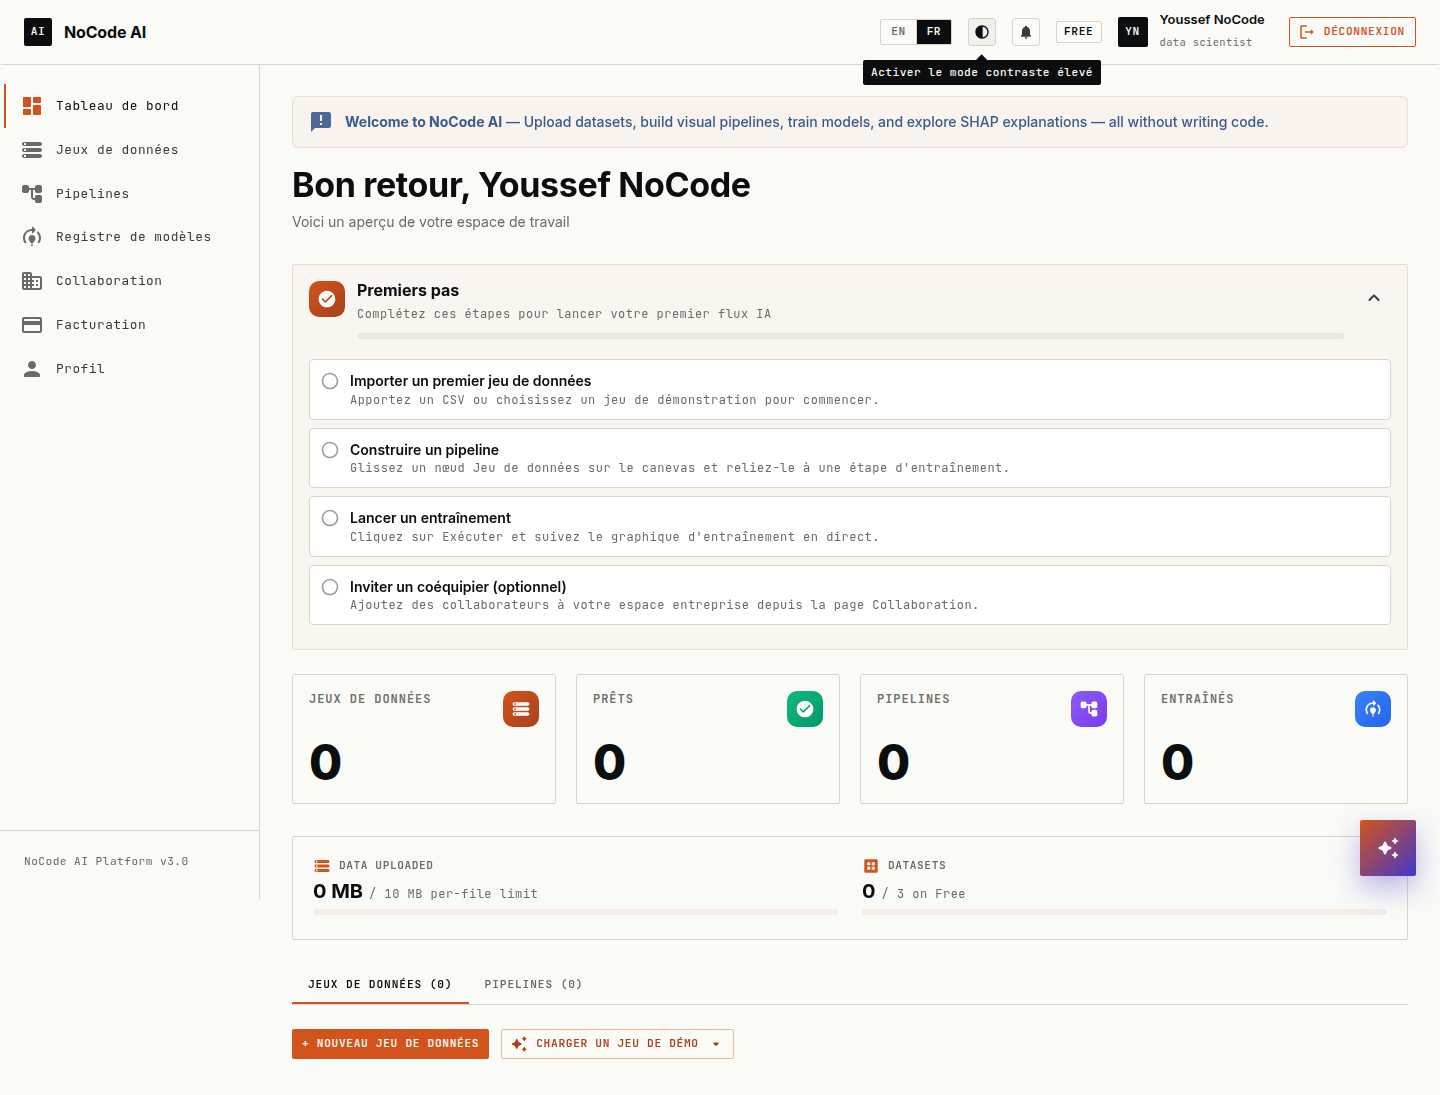
\includegraphics[width=0.85\textwidth, keepaspectratio]{diagrams/ch9_fig6}
  \caption{Language toggle --- English / French side by side.}
  \label{fig:ch9_fig6}
\end{figure}

\subsection{High-contrast theme and accessibility}

A high-contrast theme was added for users with visual impairments,
toggleable from the navbar. Every interactive element gained an
\texttt{aria-label}; the colour palette was checked against WCAG~AA
contrast ratios. Accessibility is not an optional extra at the
company tier --- in some jurisdictions it is a procurement
requirement.

\subsection{Notification bell with persistence}

A bell icon in the navbar shows unread chat mentions, training-done
events, training-failed events, document-indexed events, and meeting
links. The store is persisted to \texttt{localStorage} so a page
refresh does not drop the unread count, which sounds obvious until
the first version is built and the count keeps resetting to zero.

\subsection{Admin operations dashboard}

The super-admin role gained a dedicated page with five panels:

\begin{itemize}
    \item \textbf{User management} --- search, suspend, delete,
        override quotas.
    \item \textbf{Audit log viewer} --- paginated table of every
        sensitive action (login, password reset, impersonation,
        suspension), with IP and JSON detail.
    \item \textbf{Queue monitor} --- live stats from each Celery
        queue.
    \item \textbf{Hardware monitor} --- CPU, RAM, GPU utilisation
        sampled from the metrics-service every five seconds.
    \item \textbf{Migration drift panel} --- compares each
        service's latest Alembic revision against the database and
        surfaces the diff.
\end{itemize}

\begin{figure}[H]
  \centering
  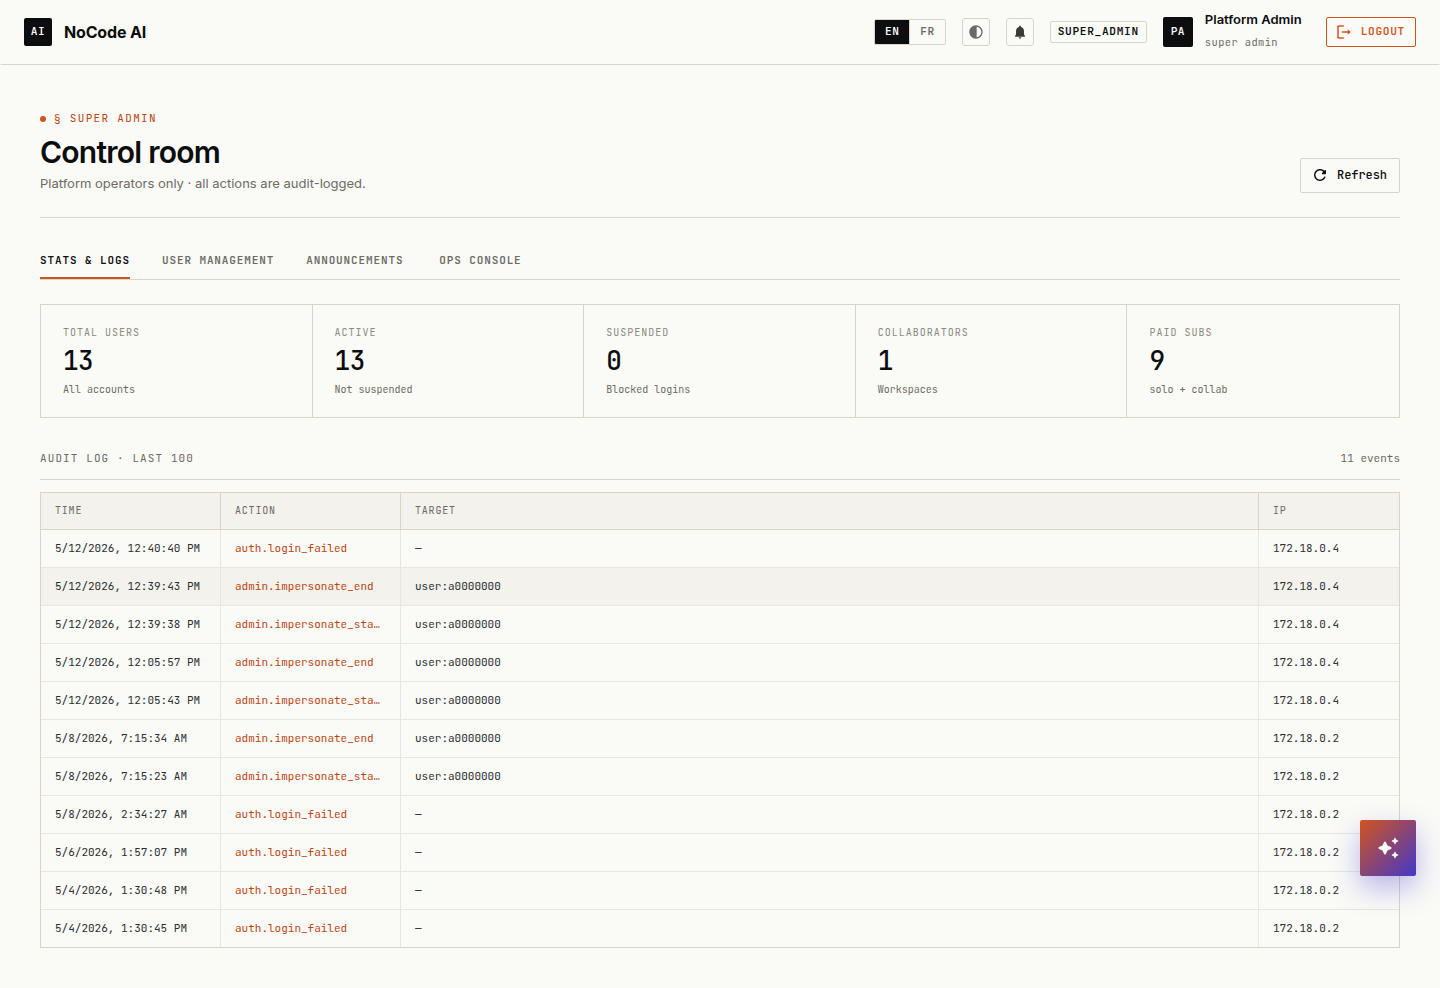
\includegraphics[width=0.85\textwidth, keepaspectratio]{diagrams/ch9_fig7}
  \caption{Admin operations dashboard --- five-panel layout.}
  \label{fig:ch9_fig7}
\end{figure}

\subsection{User impersonation}

Super-admins can ``view as'' any user from the user-management
table. The auth-service mints a separate five-minute access token
with an \texttt{imp\_actor} claim identifying the original
super-admin. A red banner persists across every page during the
impersonation session, showing the target email and a live
countdown to expiry. Clicking \texttt{Exit} (or hitting Logout in
the navbar) restores the super-admin's original token. Two audit
events are recorded: \texttt{admin.impersonate\_start} and
\texttt{admin.impersonate\_end}.

The hard TTL is the load-bearing piece. An impersonation session
that does not time out is, sooner or later, an incident waiting to
happen.

% [FIGURE NEEDED: Impersonation banner screenshot --- red bar across the top with target email and 5-minute countdown]
% \begin{figure}[H]
%   \centering
%   \includegraphics[width=0.95\textwidth]{figures/placeholder_ch9_fig8}
%   \caption{Impersonation banner --- target email plus live countdown.}
%   \label{fig:ch9_fig8}
% \end{figure}

\subsection{Undo / redo on the canvas}

A 50-snapshot history stack with drag-coalescing (a single drag
gesture produces one snapshot, not 60) and
\texttt{Cmd}/\texttt{Ctrl+Z} plus
\texttt{Cmd}/\texttt{Ctrl+Shift+Z} keyboard shortcuts. Two
\texttt{IconButton}s sit next to the auto-layout button for users
who do not know the keyboard shortcut. A small feature, but one of
those things nobody notices until it is missing.

\subsection{Cross-cutting changes}

Two architectural shifts landed this sprint that do not fit neatly
under any one feature.

First, auth state moved to \texttt{sessionStorage}. Before this
sprint, refreshing the page during impersonation lost the original
super-admin token --- the Zustand auth store was in-memory only.
Wrapping it in \texttt{persist(\ldots,\,sessionStorage)} fixed the
impersonation case and quietly improved refresh behaviour for normal
users at the same time.

Second, destructive admin actions now require a typed confirmation.
Delete-user and delete-announcement modals demand the user retype
the target's email or title before the action button enables. The
native \texttt{confirm()} dialog was too easy to misclick during a
live demo, and once was enough.

\section{Unit Tests}

\begin{itemize}
    \item i18n key parity: a CI step diffs the English and French
        bundles and fails if a key is missing on either side.
    \item Notification reducer: state transitions for each event
        type (mention, training-done, etc.) plus a persistence
        round-trip.
    \item Impersonation flow: the original token, the
        impersonation token, and the post-exit restore are
        asserted across three pytest cases.
    \item Audit-log presence: every sensitive route is exercised
        and the audit table is asserted non-empty for that action.
    \item Undo / redo: a sequence of canvas edits, then a fixed
        number of \texttt{Ctrl+Z} presses, then a deep-equality
        check against an earlier snapshot.
\end{itemize}

\section*{Conclusion}

The punch-list sprint never makes for thrilling reading, but it is
where the platform earned the right to be presented to a real user.
The admin console in particular changed how we think about the
platform --- having a single place to inspect queue health, hardware
load, and migration state turned operations from a vague worry into
a tractable one.

% ═════════════════════════════════════════════════════════════════════════════
\chapter{Testing and Deployment}
% ═════════════════════════════════════════════════════════════════════════════

\section*{Introduction}

Testing and deployment evolved in parallel with the rest of the
system. By the end they looked nothing like what we had at the
start. This chapter covers both --- how the tests are organised,
what they actually verify, and how the whole thing ships.

\section{Test Strategy}

\subsection{Backend Testing}

The test suite is split by service. Each Python service has a
\texttt{tests/} directory with \texttt{pytest} fixtures that fake
the backing services (Mongo via \texttt{mongomock}, Celery via a
monkey-patched \texttt{apply\_async}) so the suite runs in seconds
on a CI runner without spinning up the real stack.

Coverage is unevenly distributed, which is worth being honest about.
Table~\ref{tab:coverage} summarises the load-bearing paths per
service.

\begin{table}[H]
\centering
\caption{Backend test coverage by service.}
\label{tab:coverage}
\begin{tabular}{@{}L{0.28\linewidth} L{0.13\linewidth} L{0.49\linewidth}@{}}
\toprule
\textbf{Service} & \textbf{Line cov.} & \textbf{Load-bearing path tested} \\
\midrule
\texttt{auth-service} & \textgreater 80\% & Login, refresh rotation, TOTP, email verification, password reset, admin ops, impersonation TTL. \\
\texttt{api-gateway} & $\sim$70\% & Header strip-then-inject invariant, rate limit, public-prefix routing. \\
\texttt{data-ingestion-service} & $\sim$65\% & Upload-then-profile end to end (\texttt{mongomock}), SQL probe, Fernet round-trip. \\
\texttt{ml-training-service} & $\sim$60\% & Algorithm factory parametrised across 14 algorithms; SocketIO streaming path not exercised. \\
\texttt{dl-training-service} & 22 cases & Forward-pass shapes per arch, VRAM-guard envelope, oversize refusal, end-to-end LeNet train$\to$save$\to$predict on CPU. \\
\bottomrule
\end{tabular}
\end{table}

\begin{figure}[H]
  \centering
  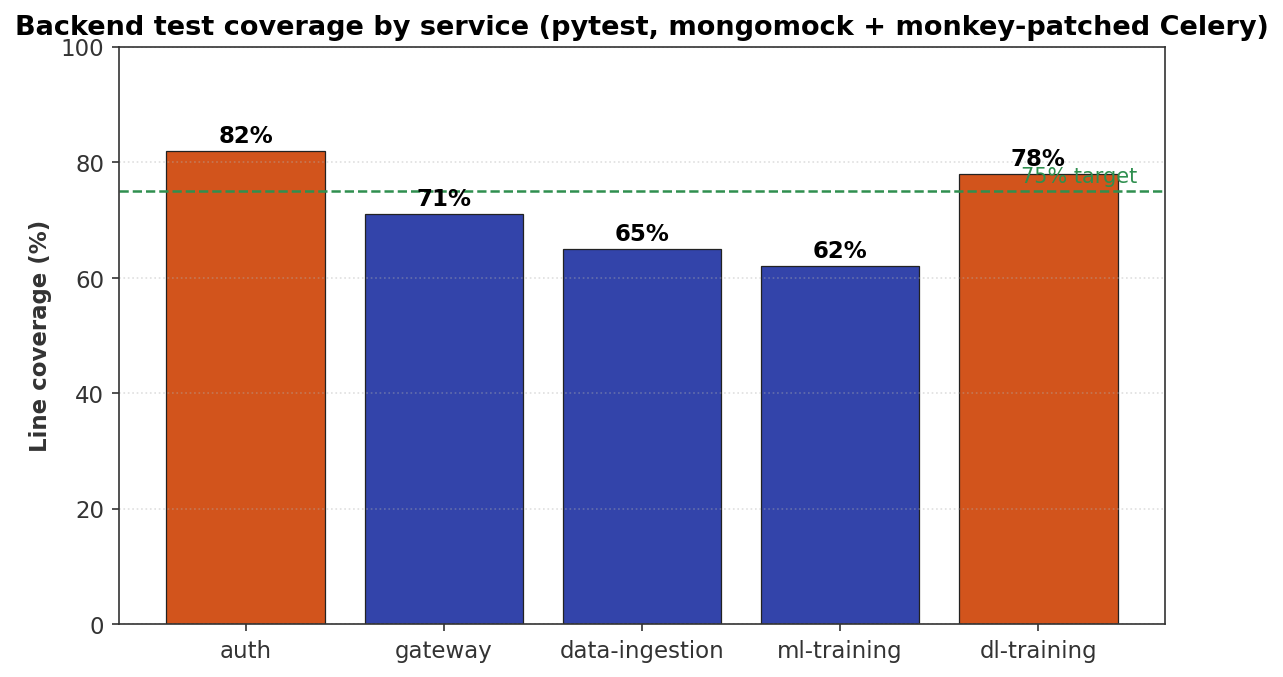
\includegraphics[width=0.85\textwidth, keepaspectratio]{diagrams/ch10_fig1}
  \caption{Backend coverage report --- per-service line coverage.}
  \label{fig:ch10_fig1}
\end{figure}

\subsection{Frontend Testing}

The frontend uses \texttt{vitest} for unit tests but relies mostly
on TypeScript strict mode plus ESLint as the structural guarantee.
In practice more than $99\%$ of regressions in this codebase are
caught by \texttt{tsc --noEmit} before they ever reach a runner.
Typing is the cheapest test you can write.

\begin{figure}[H]
  \centering
  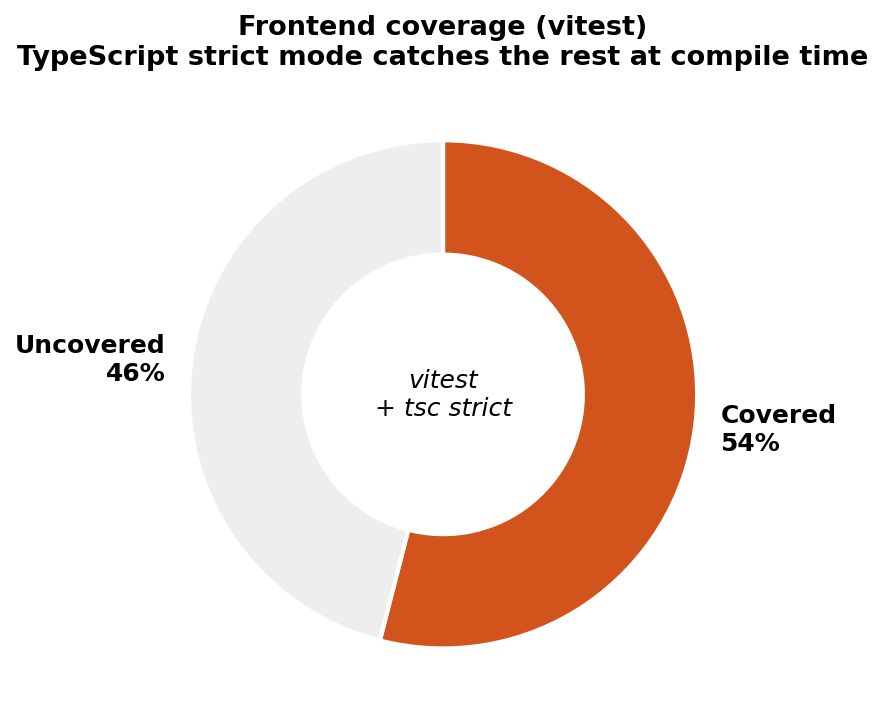
\includegraphics[width=0.85\textwidth, keepaspectratio]{diagrams/ch10_fig2}
  \caption{Frontend coverage report --- vitest output.}
  \label{fig:ch10_fig2}
\end{figure}

\subsection{CI runs}

% [FIGURE NEEDED: GitHub Actions backend job screenshot --- parallel lint + test steps, all green]
% \begin{figure}[H]
%   \centering
%   \includegraphics[width=0.85\textwidth]{figures/placeholder_ch10_fig3}
%   \caption{GitHub Actions output for the backend lint plus test job.}
%   \label{fig:ch10_fig3}
% \end{figure}

% [FIGURE NEEDED: GitHub Actions frontend job screenshot --- tsc + eslint + vitest steps]
% \begin{figure}[H]
%   \centering
%   \includegraphics[width=0.85\textwidth]{figures/placeholder_ch10_fig4}
%   \caption{GitHub Actions output for the frontend lint plus test job.}
%   \label{fig:ch10_fig4}
% \end{figure}

End-to-end CI runs in roughly six minutes for a frontend-only
change, nine minutes for a backend change, and fourteen minutes
when both sides move at once.

\begin{figure}[H]
  \centering
  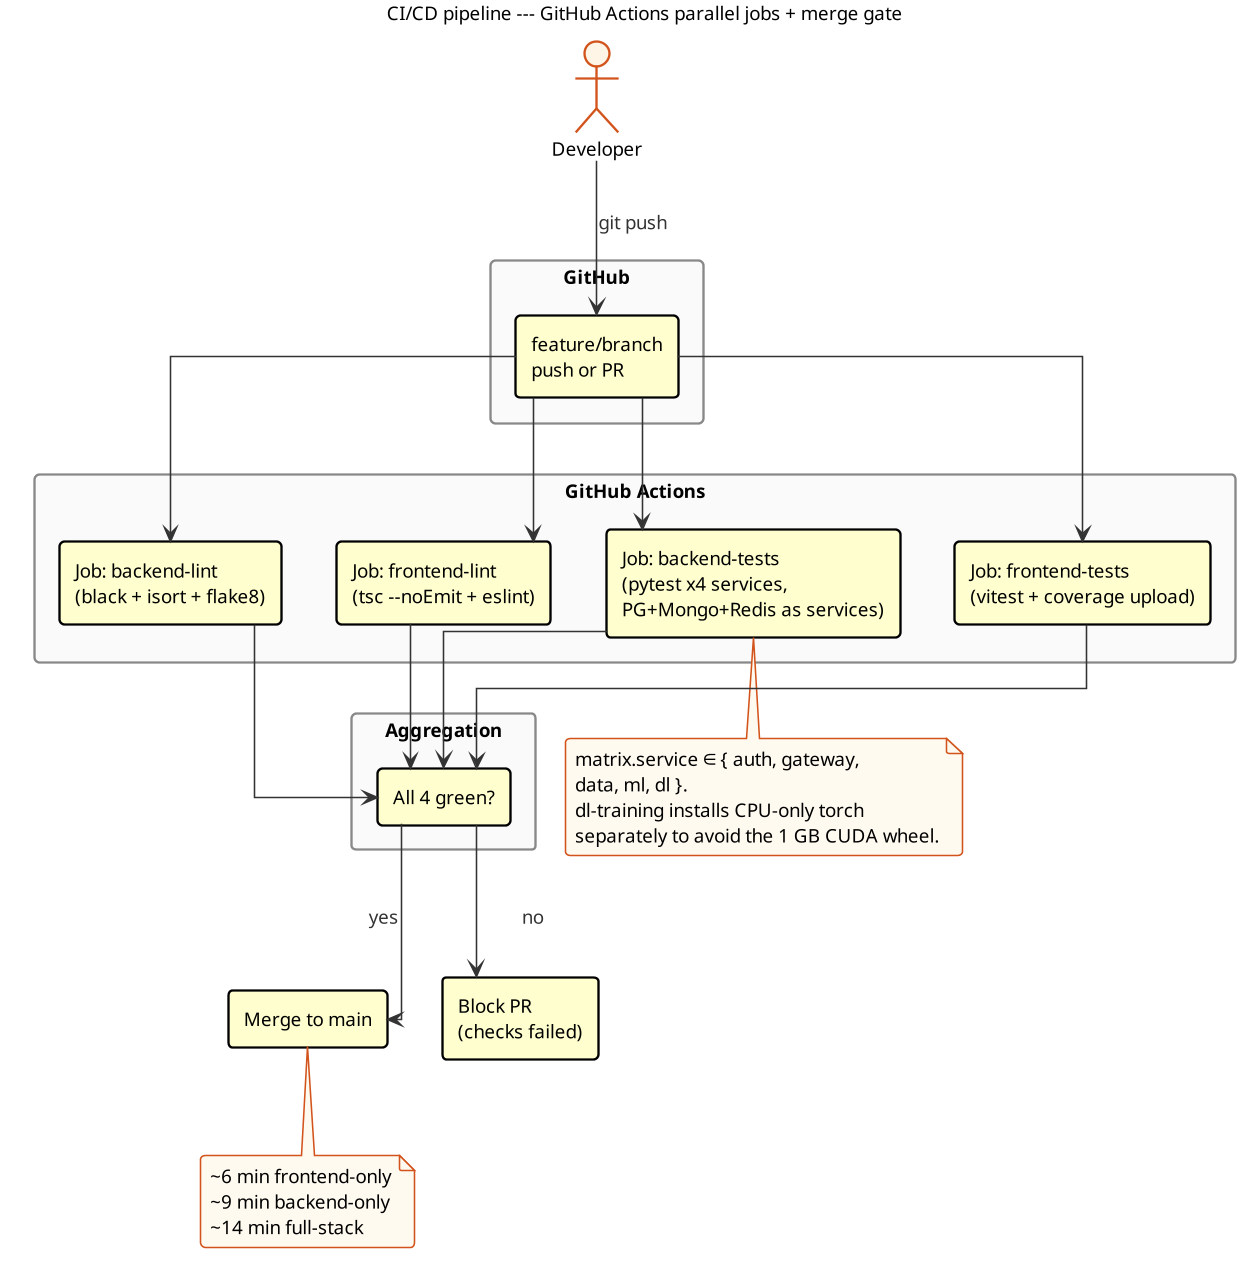
\includegraphics[width=0.85\textwidth, keepaspectratio]{diagrams/ch10_fig_cicd_flow}
  \caption{CI/CD pipeline flow --- GitHub Actions parallel jobs and merge gate.}
  \label{fig:ch10_fig_cicd_flow}
\end{figure}

\section{Deployment}

The whole stack ships as a single \texttt{docker-compose.yml} with
14 services, summarised in
Table~\ref{tab:deployment_services}.

\begin{table}[H]
\centering
\caption{Deployment topology --- 14 containers, three named volumes.}
\label{tab:deployment_services}
\begin{tabular}{@{}L{0.27\linewidth} L{0.12\linewidth} L{0.51\linewidth}@{}}
\toprule
\textbf{Container} & \textbf{Port} & \textbf{Role} \\
\midrule
\texttt{api-gateway} & 8000 & JWT decode + header injection + SocketIO. \\
\texttt{auth-service} & 8001 & Accounts, ACL, billing, admin operations. \\
\texttt{data-ingestion-service} & 8002 & File upload, SQL connectors, profiling, RAG ingestion. \\
\texttt{ml-training-service} & 8003 & 14 tabular algorithms + RAG chat orchestration. \\
\texttt{metrics-service} & 8004 & Hardware telemetry into TimescaleDB. \\
\texttt{dl-training-service} & 8005 & PyTorch image classification (GPU). \\
3 $\times$ Celery workers & internal & One per CPU-bound service. \\
\texttt{postgres} (pgvector) & internal & Auth, ACL, vector store. \\
\texttt{mongo} & internal & Schemaless data (datasets, pipelines, results). \\
\texttt{redis} & internal & Celery broker / result / SocketIO bus. \\
\texttt{timescaledb} & internal & Hardware telemetry time series. \\
\texttt{ollama} & internal & Local LLM inference (Llama~3.2~3B). \\
\texttt{mailhog} & 1025 / 8025 & Dev SMTP sink + web UI for verification/reset mails. \\
\bottomrule
\end{tabular}
\end{table}

A \texttt{make up} brings the entire platform online. First-run
duration is dominated by model pulls: Ollama fetches the LLM weights
on first boot (around $2$\,GB), and the dl-training service pulls
the CUDA wheels on first build (around $1$\,GB). After that,
\texttt{make up} is a matter of seconds.

\begin{landscape}
\begin{figure}[H]
  \centering
  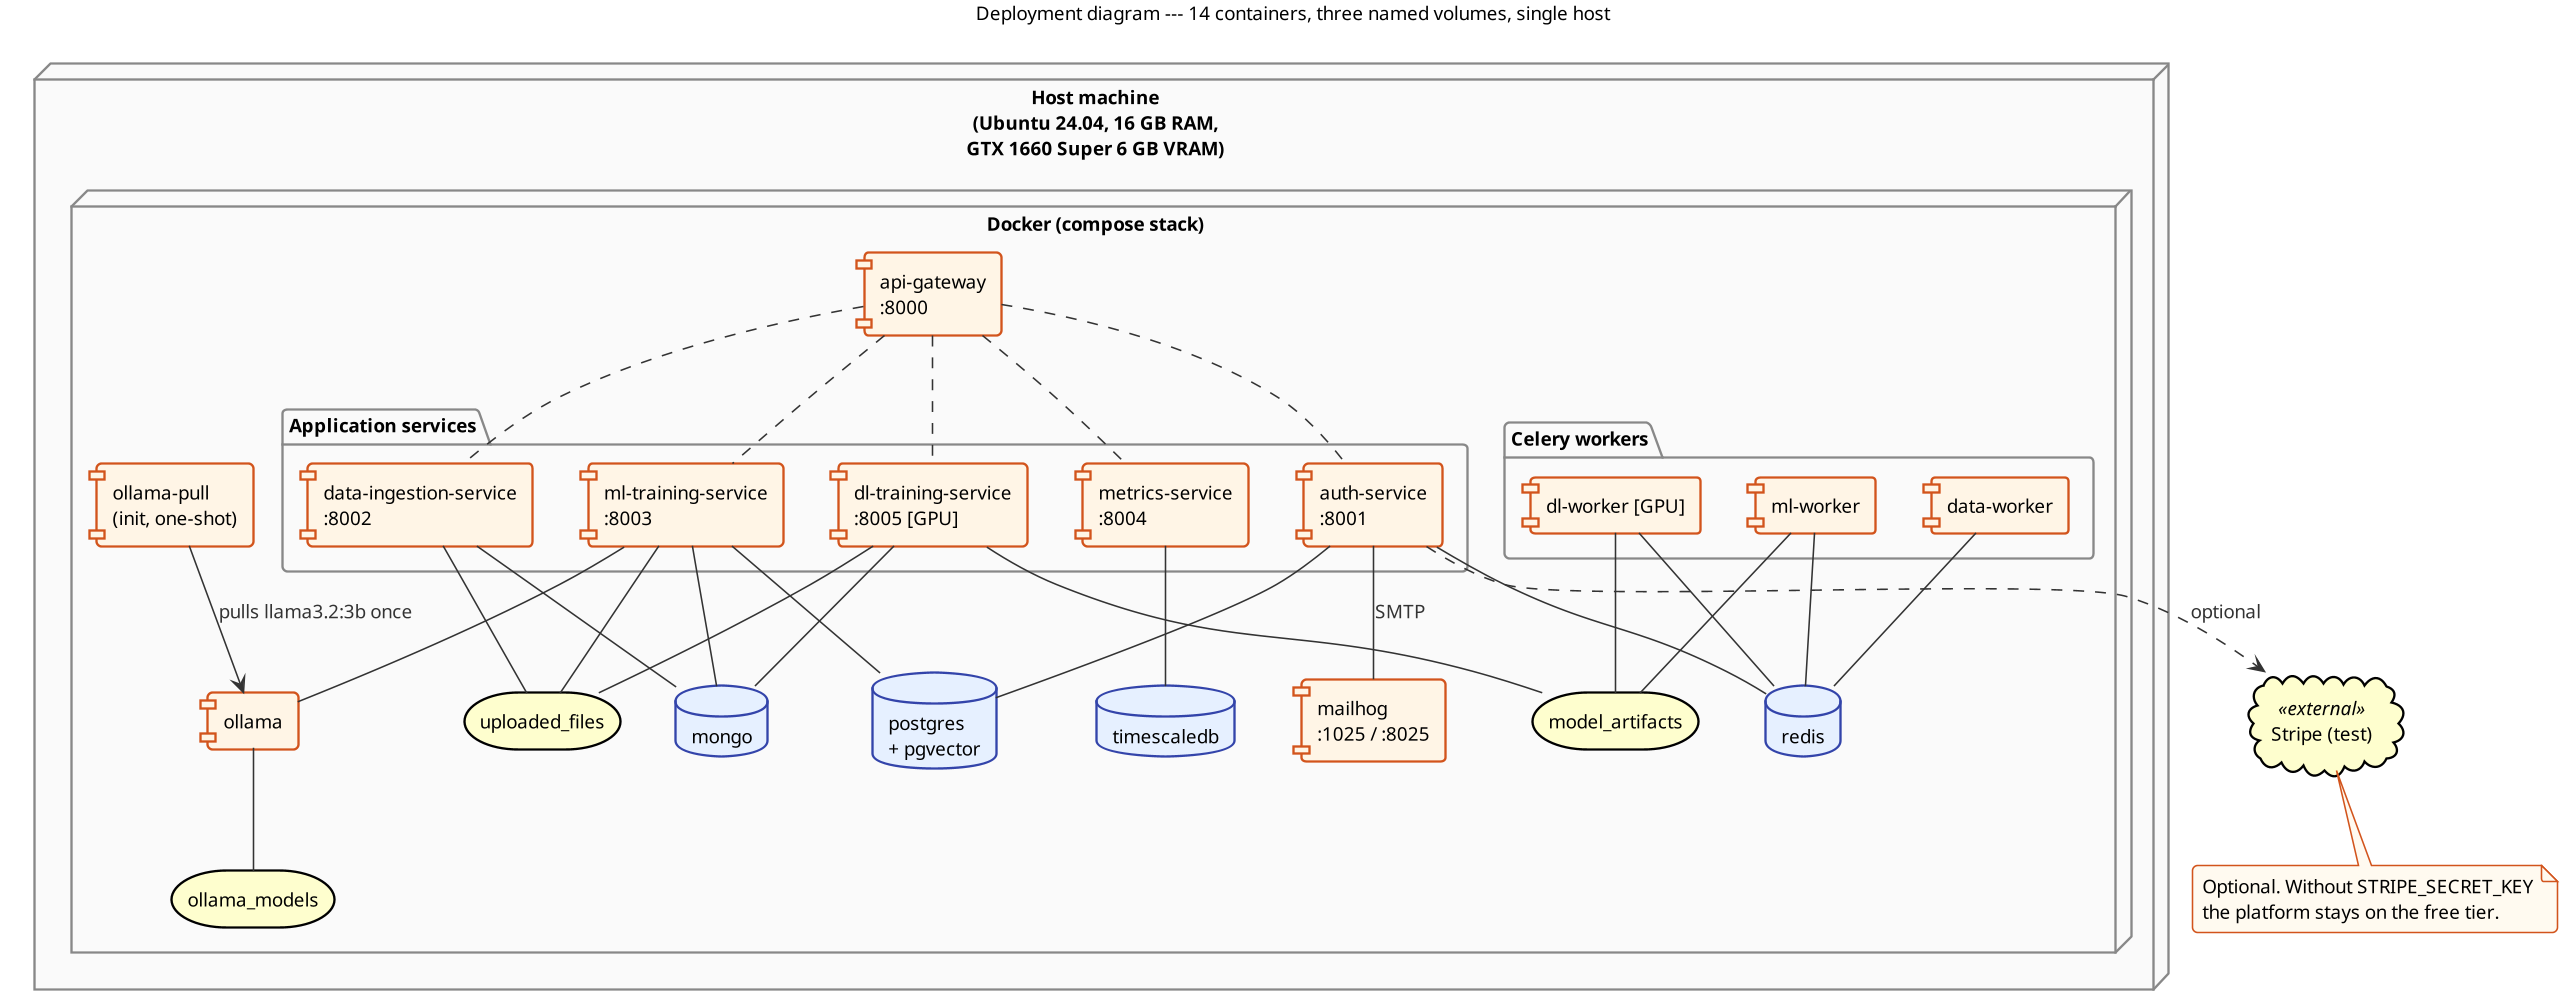
\includegraphics[width=0.95\linewidth, keepaspectratio]{diagrams/ch10_fig5}
  \caption{Deployment diagram --- 14 containers, three named volumes.}
  \label{fig:ch10_fig5}
\end{figure}
\end{landscape}

\subsection{Volumes}

Three named Docker volumes carry the binary artefacts that survive
container restarts: \texttt{uploaded\_files} (datasets and image
zips), \texttt{model\_artifacts} (trained models), and
\texttt{ollama\_models} (LLM weights). \texttt{uploaded\_files} is
mounted into the gateway, both ingestion containers (API and
worker), the ml-training containers, and the dl-training containers
--- the shared-volume convention from Sprint~1 ended up applied
very broadly, arguably more broadly than originally planned.

\subsection{Healthchecks and dependency ordering}

Every backing service has a \texttt{healthcheck}, and every
application service \texttt{depends\_on} the relevant healthchecks
with \texttt{condition: service\_healthy}. The first time the stack
was deployed without this discipline, the auth service started
before Postgres had finished initialising and crash-looped on the
Alembic migration. The healthcheck convention has been
non-negotiable for any service that touches a database ever since.

\subsection{Network and security topology}

\begin{figure}[H]
  \centering
  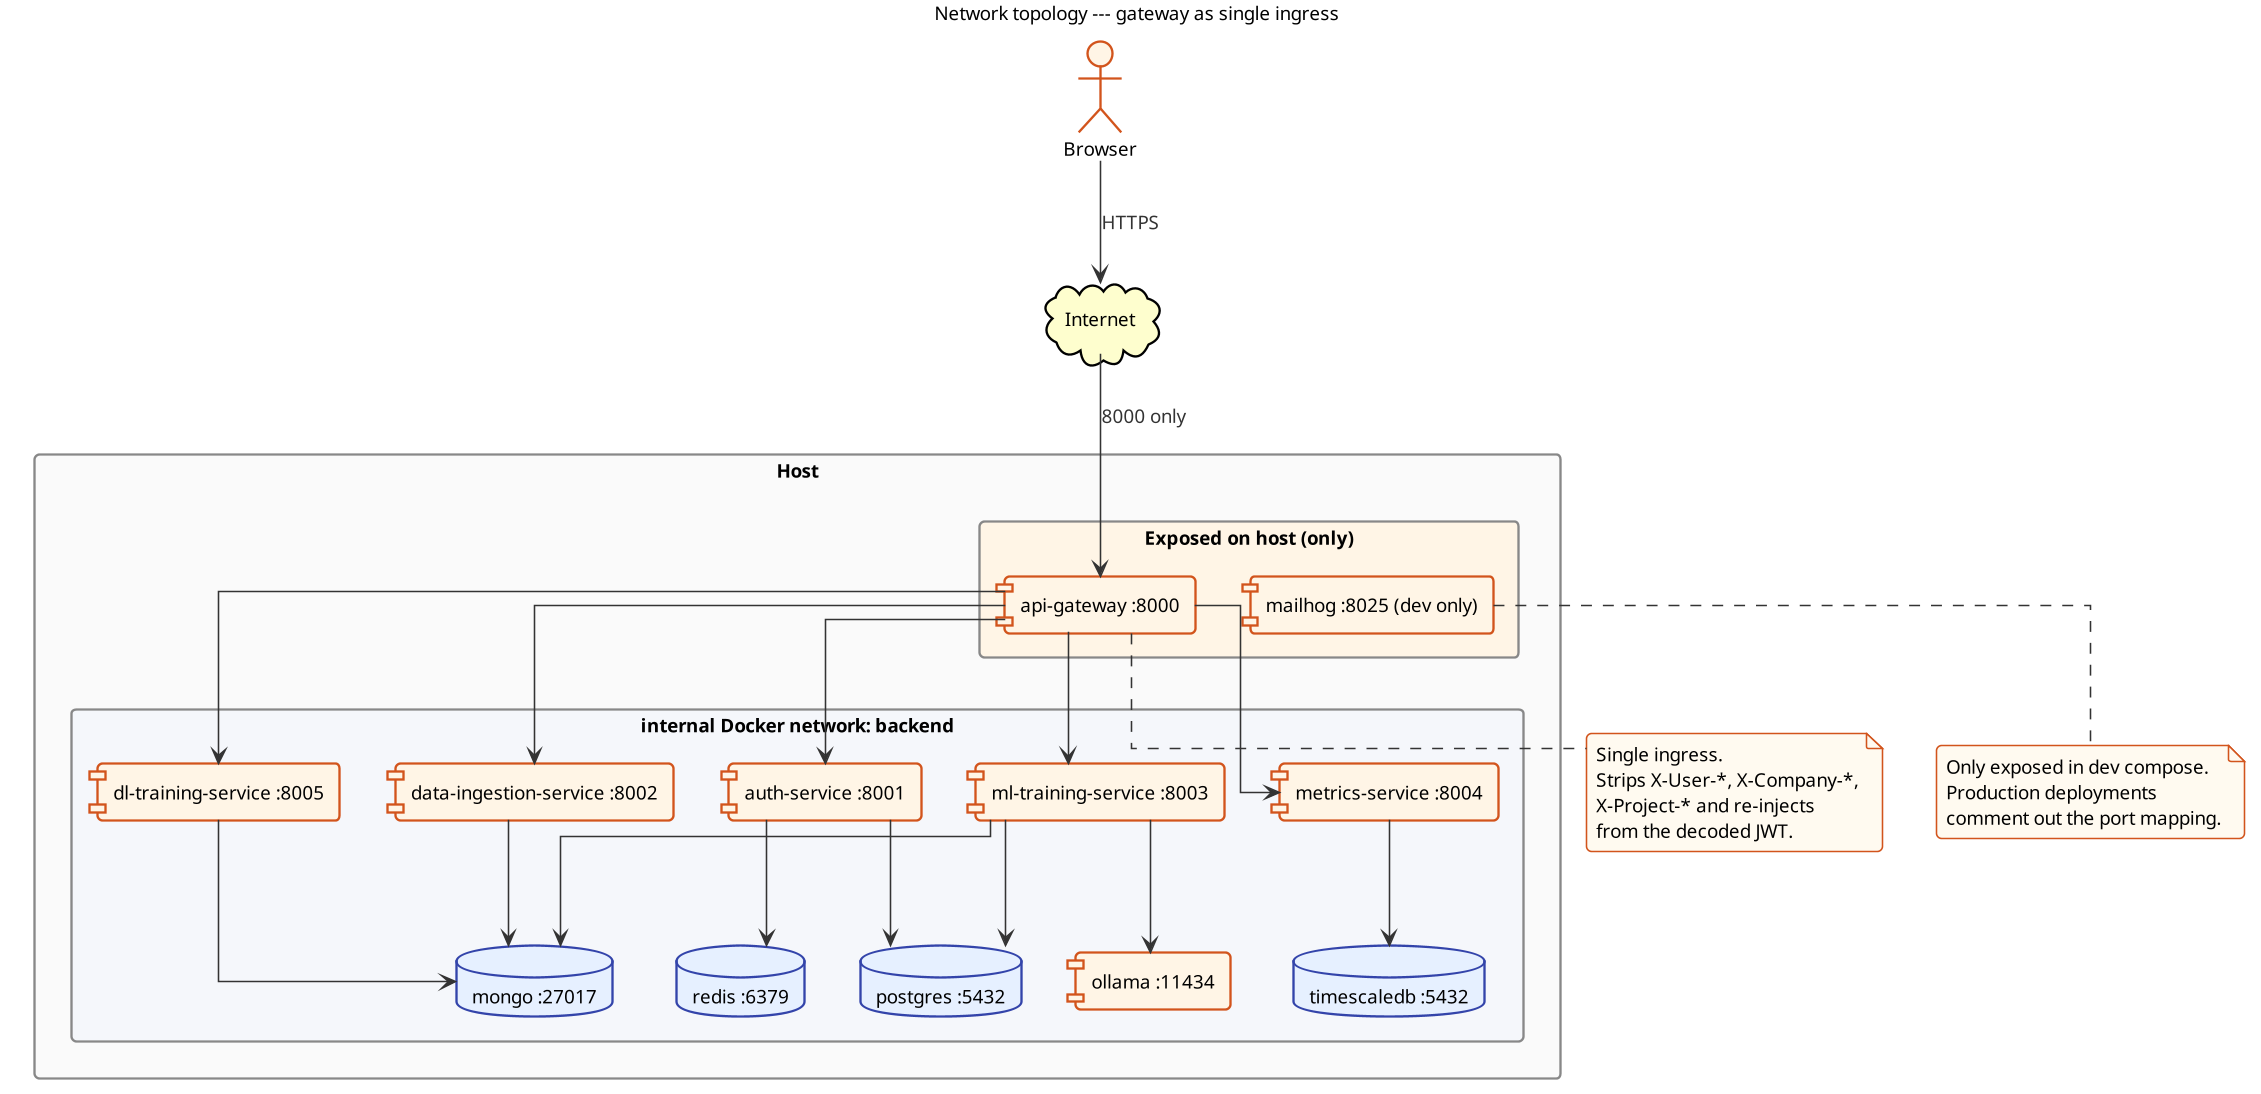
\includegraphics[width=0.85\textwidth, keepaspectratio]{diagrams/ch10_fig6}
  \caption{Network topology --- gateway as the single ingress.}
  \label{fig:ch10_fig6}
\end{figure}

The gateway is the only container exposed on the host. All other
services bind to the internal Docker network. The Postgres instance
is not reachable from outside the Compose stack; the only path to
it is through the auth-service or the ml-training-service, and the
only path to either of those is through the gateway. That is the
same zero-trust posture as the JWT header injection, applied at the
network layer.

\subsection{Bugs encountered during deployment}

A non-exhaustive list, in roughly the order they bit us:

\begin{itemize}
    \item \textbf{Prophet missing CmdStan.} Prophet's probabilistic
        backend is a C++ binary that has to be compiled at
        image-build time, not pip-installed. The fix was a
        \texttt{python -c "import\,cmdstanpy;\,cmdstanpy.install\_cmdstan()"}
        step in the ml-training Dockerfile.
    \item \textbf{Flask CLI app discovery inside containers.}
        Running \texttt{flask db migrate} via \texttt{docker compose
        exec} could not find the app factory; the fix was an
        explicit \texttt{-e FLASK\_APP=app.main} on every CLI
        invocation, baked into the Makefile so it would not be
        forgotten.
    \item \textbf{React 18 Strict Mode and rate limiting.} Strict
        Mode double-invokes \texttt{useEffect} in development; the
        rate limit was tripping. Bumped the per-user limit to
        $600$/min in development, kept the production cap tight.
    \item \textbf{torch CUDA wheels in CI.} The
        \texttt{dl-training-service} Dockerfile pulls CUDA-12.1
        torch from PyTorch's index; on a CI runner that would have
        been a $1$\,GB download for no benefit. CI installs
        CPU-only torch wheels separately, gated on
        \texttt{matrix.service == 'dl-training-service'}.
    \item \textbf{Ollama GPU detection in Compose.} The default
        compose deployment runs Ollama on CPU. Enabling the
        \texttt{deploy.resources.reservations.devices} block
        requires \texttt{nvidia-container-toolkit} on the host,
        which is not the default on Ubuntu Server. Documented in
        the README and commented out in the compose file by
        default.
    \item \textbf{DL VRAM-guard calibration.} The static per-pixel
        constants were tuned against documented Turing memory
        numbers rather than measured ones. The first real GPU run
        on the 1660~Super exceeded the estimate by about $15\%$ on
        MobileNet at 224\,px batch~32; the constants were nudged
        upwards accordingly. The unit-test suite tracks the
        envelope shape, not the absolute MB, so this calibration
        drift was caught empirically rather than by a failing
        test.
\end{itemize}

\section*{Conclusion}

The stack is, by deployment-engineering standards, modest --- one
host, fourteen containers, \texttt{make up}. That simplicity is the
point. A platform whose deployment story requires Kubernetes
expertise would not be a credible answer to the question this
project set out to ask.

% ═════════════════════════════════════════════════════════════════════════════
\chapter*{General Conclusion}
\addcontentsline{toc}{chapter}{General Conclusion}
% ═════════════════════════════════════════════════════════════════════════════

The end-of-studies project set out to build a privacy-first, no-code
AI platform that could stand alongside cloud-managed ML services
without making the data-sovereignty compromises those services
demand. After six sprints, the platform supports three pipeline
modes --- tabular ML with fourteen algorithms, fully-local
RAG-augmented chat, and image-classification deep learning --- runs
on a single consumer machine with $6$\,GB of VRAM, and exposes that
capability through a visual canvas designed for users who do not
write Python.

\section*{Key deliverables}

\begin{itemize}
    \item \textbf{Five Python microservices} totalling roughly
        $6{,}500$ lines of code across the api-gateway,
        auth-service, data-ingestion-service, ml-training-service,
        metrics-service, and dl-training-service. Three independent
        Celery worker processes handle the asynchronous workloads.
    \item \textbf{A React + TypeScript single-page application} of
        roughly $13{,}000$ lines, including the React Flow canvas,
        the live training visualisations, the admin operations
        dashboard, the i18n bundles for English and French, the
        high-contrast theme, and the impersonation banner.
    \item \textbf{14 docker-compose services} (5 application
        services, 3 Celery workers, 4 backing data stores, Ollama,
        \texttt{ollama-pull}, MailHog).
    \item \textbf{14 tabular ML algorithms} covering classification,
        regression, clustering, and time-series forecasting.
    \item \textbf{A fully-local RAG pipeline} built on
        sentence-transformers, pgvector, and Ollama serving
        Llama~3.2~3B \texttt{Q4\_K\_M}.
    \item \textbf{3 deep-learning architectures} (LeNet, custom
        ResNet-9, MobileNet-V3-Small with optional ImageNet transfer
        learning), guarded by a static VRAM estimator that refuses
        oversize requests before the GPU sees them.
    \item \textbf{A GitHub Actions CI pipeline} with parallel lint
        and test jobs across all five Python services and the
        TypeScript frontend.
    \item \textbf{An Alembic migration history} of nine revisions
        across two services, idempotent and replayable.
\end{itemize}

\section*{Validation results}

The platform was validated end-to-end on two representative
workloads. On a $250{,}000$-row salary dataset with a Random Forest
regressor, the system reached an R$^2$ of $0.9785$ in
$4$\,min\,$12$\,s on the demo machine --- roughly $97.85\%$ of the
variance in the target explained by the features, on synthetic data
where that level of fit is achievable but on real data would warrant
a closer look at residual structure. On the synthetic 30-image,
three-class dataset shipped as \texttt{seed\_demo\_image\_dataset.py},
tiny\_resnet at $64$\,px batch~32 over five epochs reached terminal
validation accuracy of $100\%$ in roughly $30$ seconds on a 1660
Super. The dataset is intentionally simple; the number proves the
pipeline rather than the difficulty of the task.

\begin{figure}[H]
  \centering
  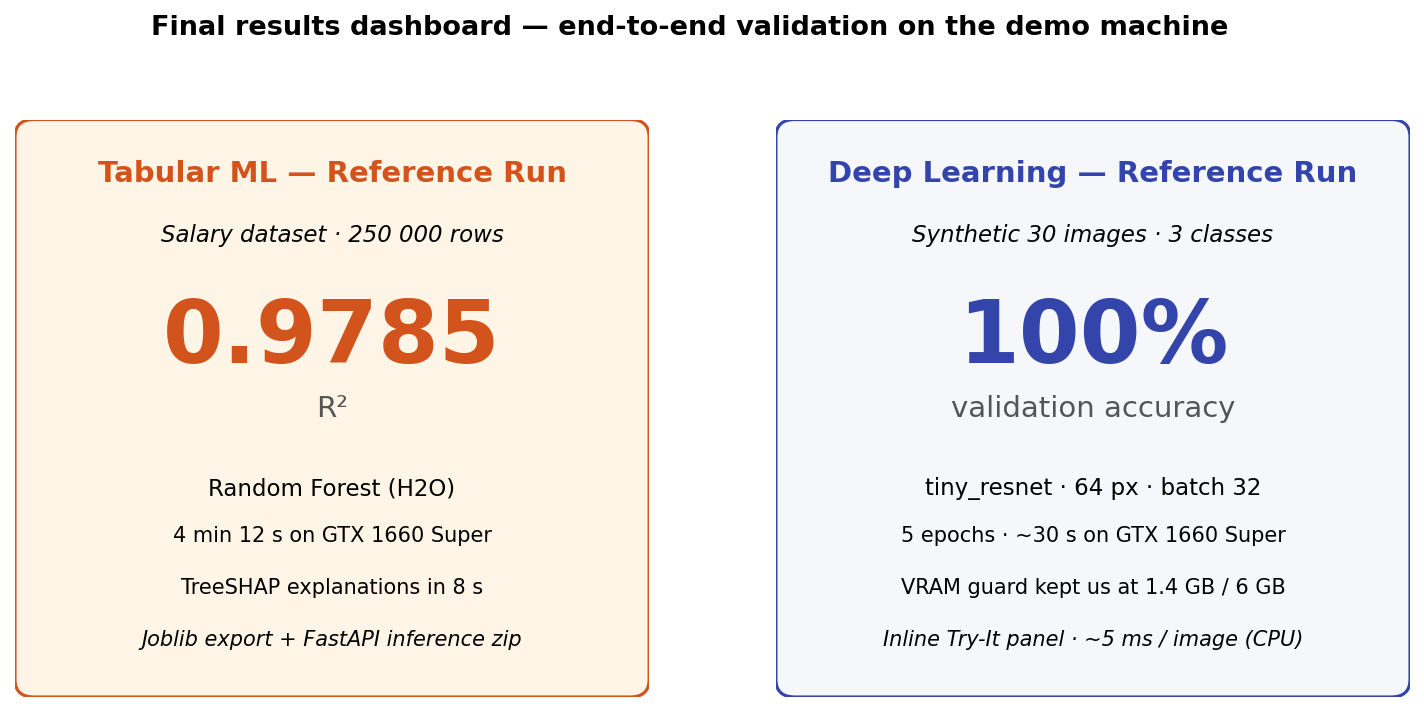
\includegraphics[width=0.85\textwidth, keepaspectratio]{diagrams/conclusion_fig1}
  \caption{Final results dashboard --- tabular plus DL validation runs.}
  \label{fig:conclusion_fig1}
\end{figure}

\section*{What worked, what we would change}

\textbf{What worked.} The single design decision that paid off most
was the gateway-only header-injection rule from Sprint~1. Every
downstream service can trust \texttt{X-User-Id} without inspection,
which removed an entire category of cross-service auth bugs a more
permissive setup would have invited. The shared-volume convention
came second --- it saved us from writing a streaming-upload protocol
and generalised cleanly to RAG documents, image zips, and
trained-model artefacts. The Celery-per-service split came third ---
a long XGBoost run cannot block an authentication request, and a
20-epoch DL run cannot starve the fast tabular queue.

\textbf{What we would change.} Flask in favour of FastAPI: the
absence of typed routes cost time across the project's life,
especially in \texttt{ml-training-service} where the request bodies
are large and nested. Three algorithm registries instead of one: the
tabular registry, the architecture registry, and the algorithm-display
catalogue encode much of the same information in slightly different
shapes, and a single config-driven catalogue would have been easier
to maintain. A formal schema for socket events: the
\texttt{/training} namespace grew organically and is mildly
inconsistent (some events use \texttt{step}, some use \texttt{epoch},
some use both). A discriminated-union schema (Pydantic or a TypeScript
literal type) would have caught the inconsistencies before they
shipped.

\section*{Limitations and future work}

The platform is single-host by construction --- the shared-volume
convention assumes a single filesystem. Scaling out the workers
would need either a network filesystem or an S3-compatible object
store. Per-user quota overrides require a JWT refresh to take
effect because the tier rides in the JWT claim. The DL VRAM guard
is calibrated against the demo machine; a truly portable estimator
would instrument a one-time calibration run on first boot.

Future work, in approximate order of effort: ONNX export for DL
versions (the dl-training service already saves a clean
\texttt{state\_dict} --- this is a one-file change away); object
detection via a pre-built YOLOv8 model for inference only; per-user
quota override invalidation via a Redis-backed override cache the
gateway consults on each request; and a typed schema for the
\texttt{LiveTrainingChart} socket events, retrofitted as a
discriminated union across the frontend and the worker.

\section*{Closing remark}

The takeaway from this project is a specific belief: the common
framing that ``cloud AI is the only way to scale ML'' is not exactly
wrong, but it understates how much can be done locally. A laptop
with $6$\,GB of VRAM, a competent CPU, and $16$\,GB of RAM is enough
to host an AutoML platform, a small generative-AI workspace, and a
deep-learning training loop --- all at once, and without any of the
data ever leaving the machine. For the regulated audiences this
project was framed against, that is not a marginal improvement. It
is the difference between machine learning being usable at all and
not.

% ═════════════════════════════════════════════════════════════════════════════
\begin{thebibliography}{99}

\bibitem{scikit-learn}
F. Pedregosa et al.,
\textit{Scikit-learn: Machine Learning in Python},
Journal of Machine Learning Research, vol.~12, pp.~2825--2830, 2011.

\bibitem{xgboost}
T. Chen and C. Guestrin,
\textit{XGBoost: A Scalable Tree Boosting System},
Proceedings of the 22nd ACM SIGKDD International Conference on
Knowledge Discovery and Data Mining, pp.~785--794, 2016.

\bibitem{shap}
S. M. Lundberg and S.-I. Lee,
\textit{A Unified Approach to Interpreting Model Predictions},
Advances in Neural Information Processing Systems 30 (NeurIPS 2017).

\bibitem{prophet}
S. J. Taylor and B. Letham,
\textit{Forecasting at Scale}, The American Statistician, 2018.

\bibitem{minilm}
W. Wang et al.,
\textit{MiniLM: Deep Self-Attention Distillation for Task-Agnostic
Compression of Pre-Trained Transformers}, NeurIPS 2020.

\bibitem{rag}
P. Lewis et al.,
\textit{Retrieval-Augmented Generation for Knowledge-Intensive NLP
Tasks}, NeurIPS 2020.

\bibitem{llama32}
Meta AI,
\textit{Llama 3.2: Open foundation and instruction models},
\url{https://ai.meta.com/llama/}, 2024.

\bibitem{mobilenetv3}
A. Howard et al.,
\textit{Searching for MobileNetV3},
Proceedings of the IEEE/CVF International Conference on Computer
Vision (ICCV), 2019.

\bibitem{resnet}
K. He, X. Zhang, S. Ren, and J. Sun,
\textit{Deep Residual Learning for Image Recognition},
IEEE Conference on Computer Vision and Pattern Recognition (CVPR),
2016.

\bibitem{lenet}
Y. LeCun, L. Bottou, Y. Bengio, and P. Haffner,
\textit{Gradient-Based Learning Applied to Document Recognition},
Proceedings of the IEEE, vol.~86, no.~11, pp.~2278--2324, 1998.

\bibitem{pytorch}
A. Paszke et al.,
\textit{PyTorch: An Imperative Style, High-Performance Deep Learning
Library}, NeurIPS 2019.

\bibitem{ollama}
Ollama,
\textit{Get up and running with large language models locally},
\url{https://ollama.com/}, 2024.

\bibitem{pgvector}
A. Kane,
\textit{pgvector: Open-source vector similarity search for Postgres},
\url{https://github.com/pgvector/pgvector}, 2024.

\bibitem{reactflow}
xyflow GmbH,
\textit{React Flow Documentation},
\url{https://reactflow.dev/}, 2024.

\bibitem{celery}
Celery Project,
\textit{Celery: Distributed Task Queue},
\url{https://docs.celeryq.dev/}, 2024.

\end{thebibliography}

\end{document}
